% ============================================================================
% MERGED PAPER (v2): Benchmarking + Engineering Simplicity
% Master file. Architecture per plan/plan.md (ranking-centric, Design B + grafts).
% Build: pdflatex auction-v2 && bibtex auction-v2 && pdflatex auction-v2 && pdflatex auction-v2
% ============================================================================
% BUILD LOG (integrator pass, 2026-07-07 -- post-restructure merge)
% - RESTRUCTURE STATUS: COMPLETE. DA demoted to appendix robustness domain
%   (app:da, full lever grid + E7 menu variants + E9 decision-level accounting);
%   Section 7 rewritten as ordinal-vs-cardinal (sec:humans-cardinal, tab:cardinal);
%   traces subsection wired into Section 6 (sec:ranking-traces) with new
%   appendix_traces (app:traces); all E3 menu/clock-framing cells four-model;
%   F3 baseline-provenance declaration in 01/04; frontier tier rebuilt on the
%   7 genuine gpt-5-mini cells (with_explanation tree disowned as GPT-4o).
% - Compile status: CLEAN. 0 LaTeX errors; 0 undefined citations/references;
%   0 multiply-defined labels; 0 bibtex errors/warnings.
% - Output: 107 pages (auction-v2.pdf).
% - Overfull hboxes: all >30pt fixed (worst remaining ~29.9pt, 04_design).
% - Figures: all real; \MISSINGFIG count 0. New assets: ranking_forest.pdf,
%   figure3_intervention_comparison.png (2x4, dollars), 4 eBay PNGs (200dpi,
%   width-based sizing), da_vs_osp.png. fig3_forward_da.pdf is now orphaned
%   (formerly in 06; app:da uses da_vs_osp.png instead) -- delete or adopt.
% - \TODO count: 31, all deliberate. Pending-experiments (need runs/API keys):
%   E2 IPV-clock re-run + clock K top-up (01/04/06/appendix_procedures);
%   E4 Gemma fidelity battery (04/05/appendix_ablations); E8 harmonized
%   baselines (04/appendix_ablations/appendix_prospect); frontier intervention
%   battery, runbook at plan/FRONTIER_RUNBOOK.md (06/08/appendix_ablations);
%   paraphrase robustness (08); eBay r in {70,85} re-run (appendix_ebay);
%   traces cross-model FPSB/TPSB cells (06); E5/E10 CV-K pin (04).
%   Pending-analysis (no new runs): reconstruction bootstrap bands
%   (08/appendix_human/appendix_ablations); difficulty-row concordance stat
%   (05); regenerate appendix2_model_comparison.png without the misattributed
%   gpt-5-mini series (appendix_ablations); Myerson reserve check (05).
%   Pending co-author decisions: trace-extension choice (appendix_traces);
%   LLM-judge trace taxonomy (06); human-study cost verification (08) --
%   RESOLVED 2026-07-08, tab:cost now cites documented subject counts/payments
%   (Li 2017: 548 subjects, ~$5,400 documented for the main experiment;
%   Gonczarowski et al. 2024: 542 subjects, $15-26/subject, Appendix A.1);
%   B3 template provenance footnote retained in 04 (naming history).
% - Known cross-file conventions locked this pass: clock rung = the
%   ascending_clock_closed cells (SMAD 1.4-5.2%, p<0.001 all four, d<=1.00);
%   clock-framing B3 = intervention_proxy_breitmoser (SMAD 6.3-13.8%, sig 3/4,
%   pooled rho +0.29); menu = sign-mixed, null on average (sign test p=0.73);
%   direction shares = repo-canonical (human 67.2% overbid of all bids, 92.2%
%   among deviators; GPT-4o 74.1% underbid, 81.6% among deviators), band
%   convention only in fig:direction with footnotes; gpt-5-mini FPSB reported
%   CSV-faithfully (RNE-consistent, +$0.002 vs b*; -$8.53 is vs value);
%   OSP-DA zero rescoped per F4 everywhere; Claude Payoff-Safety endpoint
%   +0.30 per logs (sign flag vs ES manuscript, footnoted in 06/app:traces);
%   eBay T4-beyond-T2 dampening claim removed (honest non-finding in
%   appendix_ebay); revenue null always paired with the disabled price-lift
%   caveat; DA cross-model means declared unweighted.
% - Known co-author decisions pending: (i) RESOLVED 2026-07-08 -- \ifanon build
%   now scrubs the open-source-release sentence in intro P9 (01_intro.tex) and
%   replaces the Disclosure paragraph below with an anonymized placeholder;
%   (ii) star policy: tab:winners-curse keeps significance stars (tests vs. theory,
%   not vs. reconstructed humans -- allowed under R8, flag for uniformity).
% - Local TeX note: enumitem/bbm/algorithms/algorithmicx/courier installed to
%   the user tree (~/Library/texmf) via tlmgr usermode from the TL2024 historic
%   repo; required for this machine's BasicTeX to build the master.
% ============================================================================
\documentclass{article}
\usepackage[utf8]{inputenc}
\usepackage[T1]{fontenc}
\usepackage{times}

\input{math_commands.tex}

\usepackage{amsmath}
\usepackage{amsthm}
\usepackage{graphicx}
\usepackage{float}
\usepackage{booktabs}
\usepackage{multirow}
\usepackage{tabularx}
\usepackage{array}
\usepackage{subcaption}
\usepackage{enumitem}
\usepackage{xcolor}
\usepackage{natbib}
\usepackage{geometry}
\usepackage{url}
\usepackage{bbm}
\usepackage{algorithm}
\usepackage{algpseudocode}
\usepackage{listings}
\lstset{
  basicstyle=\ttfamily\footnotesize,
  breaklines=true,
  columns=fullflexible
}
\usepackage{hyperref}
\setcitestyle{authoryear}

% Figures live in several places during the draft stage.
\graphicspath{{figures/}{../Engineering_simplicity/plots/}{../Engineering_simplicity/engineer_simplicity-main/plots/auctions/}{../Engineering_simplicity/engineer_simplicity-main/plots/da/}}

% ---------------------------------------------------------------------------
% Draft machinery
% ---------------------------------------------------------------------------
\newcount\Comments  % 0 suppresses notes-to-selves
\Comments = 1
\newcommand{\kibitz}[2]{\ifnum\Comments=1{\color{#1}{#2}}\fi}
\definecolor{english}{rgb}{0.0, 0.5, 0.0}
\newcommand{\dcpadd}[1]{\kibitz{english}{#1}}
\newcommand{\dcp}[1]{\kibitz{teal}{[DCP: #1]}}
\newcommand{\khz}[1]{\kibitz{red}{[Kehang: #1]}}
\newcommand{\kerem}[1]{\kibitz{cyan}{[kerem: #1]}}
\newcommand{\jeff}[1]{\kibitz{brown}{[jeff: #1]}}
\newcommand{\avs}[1]{\kibitz{purple}{[avs: #1]}}
% Pending-work flag: anything that awaits the harmonized re-runs (plan.md \S6)
\newcommand{\TODO}[1]{\kibitz{red}{[TODO: #1]}}
% Placeholder for a referenced figure whose asset is not yet regenerated
\newcommand{\MISSINGFIG}[1]{\fbox{\parbox{0.9\linewidth}{\centering\vspace{2em}\textcolor{red}{\textbf{FIGURE PENDING:} #1}\vspace{2em}}}}

% Anonymization toggle (plan.md R11): \anontrue for conference builds
\newif\ifanon
\anonfalse

\title{What Makes Truth-Telling Obvious? An Empirical Ranking of Simplicity-Preserving Design for LLM Agents\ifanon\else\thanks{
  \footnotesize
  This research was made possible by a generous grant from Dropbox Inc.\ Thanks to Parker Whitfill and Kobi Gal for their helpful feedback. Author's contact information, code, and data will be available at \url{https://github.com/KeHang-Zhu/llm-auction}. Anand V.\ Shah and Kehang Zhu contributed equally to this work. John J.\ Horton is a co-founder of Expected Parrot Inc., which develops generative AI models for market research applications. The views expressed herein are those of the authors and do not necessarily reflect the views of the National Bureau of Economic Research.
}\fi}

\ifanon
\author{Anonymous}
\else
\author{
  Anand Shah$^{*}$\\
  MIT \\
  \and
  Kehang Zhu$^{*}$\\
  Harvard  \\
  \and
  Yanchen Jiang \\
  Harvard \\
  \and
  Jeffrey G. Wang \\
  Harvard \\
  \and
  Arif K. Dayi \\
  Harvard \\
  \and
  John J. Horton \\
  MIT \& NBER \\
  \and
  David C. Parkes \\
  Harvard \\
}
\fi
\date{
Initial draft: May 30, 2024 \\
Current version: \today
}

\begin{document}

\maketitle

% ============================================================================
% 00_abstract.tex — merged paper (auction-v2)
% \begin{abstract}...\end{abstract} only; no citations (per CONVENTIONS §1).
% Auctions = main domain; matching demoted to one appendix clause.
% Menu claim per F1; clock-framing cross-model per F2; Section 7 (ordinal vs
% cardinal) per F9; traces dissociation per F8.
% ============================================================================
\begin{abstract}
Incentive compatibility on paper does not guarantee dominant-strategy play in practice: agents must recognize that truthful play is safe. As large language model (LLM) agents begin to transact, a design question becomes operational: which levers---the extensive form, the mechanism's description, or scaffolds for the agent's reasoning---preserve truthful play for this new bounded reasoner? We rank these levers empirically in auction environments across four LLM families, using a testbed validated against moment-matched reconstructions of human experimental data: LLM bidders reproduce the human difficulty ranking of auction formats, winner's-curse comparative statics, and last-minute bidding under hard-close rules. The levers form a stable tier structure. Obviously strategy-proof extensive forms rank at the top. Safety-exposing descriptions, clock-framing---which improves play in all four models---and contingent-reasoning scaffolds form a strong second tier; menu restatements have no consistent effect---small, sign-mixed across models, null on average; forward-planning and belief-formation scaffolds actively backfire. The active ingredient is a description's invariance content: text exposing why truth-telling is safe helps, while mechanical restatement does not---and reasoning traces show the safety description moves bids without changing stated reasoning. Human evidence agrees in sign wherever a benchmark exists, and the results replicate in a school-choice matching domain (appendix). Yet the agreement is ordinal, not cardinal: no single tuning of the agents makes their bidding match human behavior in levels across mechanisms.
\end{abstract}


\newpage

% ============================================================================
% 01_intro.tex — merged paper (auction-v2)
% Nine-paragraph skeleton per plan/plan.md §2, re-sequenced per PI directive:
% auctions = main domain, DA/matching demoted to appendix robustness; menu per
% F1; clock-framing cross-model per F2; baseline provenance declared per F3;
% OSP-DA rescoped per F4; tier structure per F5 (Kendall's W + honest menu
% boundary); frontier nuance (F6) and the Section-7 cardinal question (F9)
% folded into P8a; direction shares use the repo-canonical convention (F9).
% Sources: writeup/contents/intro.tex; Engineering_simplicity/main.tex:69–89;
% results/merged_ranking/{auction_cells_summary.md, da_cells_summary.md,
% concordance.md}; results/cardinal/cardinal_summary.md;
% results/traces/traces_summary.md.
% ============================================================================
\section{Introduction}\label{sec:intro}

% --- P1: The design question -----------------------------------------------
A mechanism can be incentive compatible on paper and still fail in the minds of its participants. Truthful bidding is the dominant strategy in the second-price sealed-bid (SPSB) auction \citep{vickrey1961counterspeculation}, and the logic is short: a bid determines only \emph{whether} the bidder wins, not \emph{what} she pays; overbidding risks paying more than value, underbidding risks losing profitable wins. Yet human subjects have failed to bid truthfully in this auction for decades \citep{kagel1993independent, kagel1995individual}. The theory of simple mechanisms was built to explain such failures: obvious strategy-proofness \citep{li2017obviously}, strategic simplicity \citep{borgers2019strategically}, and one-step simplicity \citep{pycia2023theory} characterize which \emph{implementations} of the same allocation rule make good play cognitively feasible, and \citet{li2024designing} decomposes the underlying cognitive burden into contingent reasoning, forward planning, and belief formation. As large language model (LLM) agents begin to transact---bidding in ad exchanges, negotiating on procurement platforms, submitting preference rankings on behalf of applicants---this body of theory acquires a new and operational audience. The question is no longer only which designs are simple for humans, but which of the levers available to a mechanism designer preserve dominant-strategy play for a new kind of bounded reasoner. The stakes of the question are visible in a single cell of our data: GPT-4o's average bid in an SPSB auction falls roughly \$3.3 below its value, against dominant-strategy bids averaging \$24.5\footnote{Baseline provenance, here and throughout: comparisons across mechanisms (e.g., sealed bid versus clock) use the dedicated SPSB baseline cells (mean deviations $-\$0.49$, $-\$1.63$, $-\$3.28$, $-\$5.27$ for Claude, Gemini, GPT-4o, and Gemma respectively), while presentation and scaffold contrasts use the pooled axis-1/axis-3 baseline cells run in the same grid (a provenance audit reclassified the legacy axis-2 ``baseline'' as a treated clock-framing description; Section~\ref{sec:ranking-synthesis}); both conventions are reported in the master cell dataset (Section~\ref{sec:design}).}---yet a one-sentence change in how the very same rule is \emph{described} removes roughly half of that deviation.

% --- P2: What we do ----------------------------------------------------------
This paper delivers an empirical ranking of those levers. We organize the design space into three families: changes to the \emph{extensive form} (replacing a sealed bid with an ascending clock; replacing a one-shot report with an iterative query protocol), changes to the \emph{description} of a fixed mechanism (menu restatements, safety-exposing descriptions, clock-framing), and \emph{reasoning scaffolds} appended to the agent's instructions (contingent reasoning, forward planning, belief formation); a fourth family of preference framings is studied in Appendix~\ref{app:prospect}. Our main domain is the auction laboratory: an SPSB auction with three bidders and independent private values, surrounded by the first-price, third-price, common-value, and clock formats that make cross-format comparisons possible. As a generalization check, we replicate the full lever grid in a second canonical strategy-proof domain---student-proposing deferred acceptance (DA) in a $4\times4$ school-choice market with Ergin-acyclic priorities---reported in Appendix~\ref{app:da} and drawn on below where it sharpens the auction findings. We run the grid on four model families---GPT-4o (2024-08-06), Claude 3.5 Haiku (2024-10-22), Gemini 2.0 Flash, and Gemma 27B---and summarize each lever by a \emph{preservation index} $\rho$, the fraction of the baseline deviation from dominant-strategy play that the lever removes, computed within model and domain. We anchor the exposition on GPT-4o, which remains a widely used, well-studied general-purpose model for strategic and economic reasoning tasks in the recent literature \citep{horton2023large, manning2024automated}. This is a design choice for interpretability rather than a claim about model superiority: a fixed anchor isolates variation induced by mechanism, information environment, and presentation, while the ranking itself is computed within each model, so it is invariant to cross-model level differences.\footnote{Appendix~\ref{app:ablations} brackets the capability range. A frontier reasoning model (gpt-5-mini) bids the dominant strategy almost perfectly in SPSB (SMAD 0.2\%) and shades the first-price auction almost exactly to the risk-neutral equilibrium (mean deviation from the equilibrium benchmark $+\$0.002$; $-\$8.53$ from value), yet misses the third-price equilibrium badly (SMAD 60\%)---frontier capability narrows, but does not close, the bounded-rationality regime our ranking speaks to. A small open-weight model (Llama-3-8B, SMAD 57.58\%) marks the capability floor.}

% --- P3: Why the testbed is credible ----------------------------------------
A ranking computed on LLM agents is only as informative as the testbed that produces it, and a central challenge in using LLMs for mechanism design is deciding what they should be benchmarked against. Comparing bids only to theoretical equilibrium is informative but incomplete: mechanism performance in practice depends on systematic and well-documented deviations in human behavior. Auctions are a particularly useful proving ground precisely because they combine sharp theoretical predictions---equilibrium bidding and dominant-strategy truth-telling---with a deep experimental literature documenting robust regularities and mistakes, including overbidding, winner's-curse losses, and last-minute bidding under hard-close rules \citep{kagel2020handbook}. We therefore benchmark LLM behavior against human auction data as well as against theory. Using method-of-moments reconstructions of human bidding strategies from classic experiments \citep{kagel1993independent, kagel1986winner, li2017obviously, breitmoser2022obviousness, gonczarowski2024describing} and a unified metric---the scaled mean absolute deviation (SMAD)---we show in Section~\ref{sec:validation} that the testbed reproduces the human difficulty ranking of auction formats: GPT-4o's SMAD is 27.55\% in first-price versus 8.69\% in second-price auctions, mirroring the human 24.76\% versus 5.65\%. LLM bidders also reproduce the winner's-curse comparative statics---mean winner profits in first-price common-value auctions fall from $-2.54$ with four bidders to $-5.55$ with seven, and the curse is attenuated under second-price rules---and they snipe under hard-close rules in an eBay-style environment, echoing field evidence \citep{roth2002last}. Behavior is stable across rounds, with no evidence of within-session learning, so these patterns are properties of the agents rather than artifacts of experience.

% --- P4: Ranking result 1 — OSP tops (auctions-led; DA one sentence) ----------
The first ranking result is that obviously strategy-proof (OSP) extensive forms sit alone at the top. Replacing the sealed bid with an ascending clock compresses the cross-model mean deviation from $-\$2.67$ to roughly $-\$0.5$ (cross-model means, here and throughout, are unweighted averages over the four models), cuts SMAD to 1.4--5.2\% from baselines of 9.5--20.7\% ($p<0.001$ in every model, effect sizes up to $d=1.00$), and eliminates the heavy left tail of severe underbids.\footnote{A dedicated clean-IPV clock cell (IPV description and draws, $\$0.5$ tick, $K=50$) reproduces the result exactly for the two models re-runnable at the time of writing---SMAD $1.5\%$ (GPT-4o) and $1.8\%$ (Gemma)---so the rung does not rest on the legacy cells' mislabeled environment (Section~\ref{sec:ranking-extensive}).} The pattern generalizes beyond auctions. Standard DA is strategy-proof for the proposing side \citep{roth1982economics} but generally not OSP-implementable \citep{ashlagi2018stable}; under Ergin-acyclic priorities \citep{ergin2002efficient}, an iterative query protocol is OSP, and in our matching domain it drives observable misreports to zero for three of four models in the pick-based protocol (rule-of-three 95\% upper bounds below 1\%)---to our knowledge the first experimental test of an OSP implementation of DA with any kind of agent---while a yes/no implementation of the same protocol exposes model-specific failures that the pick-based accounting cannot see (Appendix~\ref{app:da}).

% --- P5: Ranking result 2 — descriptions split by invariance content ----------
The second result is that descriptions split into two sharply different sub-families, and the split is governed by what the words \emph{contain}, not by how many of them there are. A menu restatement in the style of \citet{gonczarowski2023strategyproofness}---rewording the SPSB rule as a menu of outcomes determined by others' bids---has no consistent effect: across the four models the shift is small and sign-mixed (Gemma moves toward truthful play, $+\$2.03$, $p<0.001$; GPT-4o away, $-\$1.16$, Welch $p=0.013$; Claude marginally away; Gemini is null), and null on average (placebo sign test $p=0.73$)---consistent, on average, with the modest behavioral effects of menu descriptions in human experiments \citep{gonczarowski2024describing}, though with model heterogeneity humans were never tested for. Safety-exposing descriptions, by contrast, are powerful: stating the payoff-safety invariant of the auction---your bid determines \emph{whether} you win, not \emph{what} you pay---cuts the cross-model mean deviation from $-\$2.67$ to $-\$1.53$. Clock-framing---merely \emph{describing} the sealed bid as an automatic exit threshold on a price clock, a change of words with no change to the game---helps three of the four models, cutting GPT-4o's mean deviation from $-\$2.94$ to $-\$1.54$ and halving Gemma's ($p<0.001$ each), while pushing the fourth, Gemini, away from truthful play---a first sign of a paraphrase sensitivity that Section~\ref{sec:ranking-descriptions} measures directly. The matching domain sharpens the diagnosis (Appendix~\ref{app:da}): there, a menu description that carries the invariance statement behaves like a safety description (pooled misreport error falls from 4.2\% to 1.8\%), a menu that restates only the computational mechanics makes play \emph{worse} (4.2\% to 6.9\%), and stating the rejection-safety invariant collapses error to 0.2\%, nearly matching the full OSP implementation. The active ingredient is not rewording the rules but exposing the incentive invariant that makes truth-telling safe.

% --- P6: Ranking result 3 — scaffolds are double-edged ------------------------
The third result is that reasoning scaffolds are double-edged, and the direction of the edge is predicted by which cognitive dimension they target. Scaffolding \emph{contingent reasoning}---a payoff-tree prompt that walks the agent through what happens in each outcome it might face---improves play across the board, cutting auction deviations from $-\$2.67$ to $-\$1.13$. Scaffolding \emph{belief formation} backfires: prompting first- and second-order beliefs about opponents pushes auction deviations to $-\$3.04$ and $-\$3.47$, with the damage concentrated in the weakest models while Gemini is largely immune. A one-shot sealed bid has no forward-planning axis, so \emph{forward planning} is tested in the matching domain (Appendix~\ref{app:da}), where it backfires as well: prompting models to reason about their own future decision points in DA's rejection dynamics worsens misreport error from 4.2\% to 7.8\% under one-step lookahead. The scaffolds give models material to strategize with, but not the ability to strategize well.

% --- P7: The assembled ranking, its concordance, and its theory parallel ------
Assembled, these results form the paper's central object: an empirical simplicity-preservation hierarchy of design levers (Section~\ref{sec:ranking}, Figure~\ref{fig:ranking}, Table~\ref{tab:ranking}). The hierarchy is a \emph{tier structure}, not a strict total order: OSP extensive forms at the top; safety-exposing descriptions, clock-framing, and contingent-reasoning scaffolds in a strong second tier whose internal order flips across domains (the payoff tree beats the safety description in three of four auction cells; the safety description beats the tree in all four matching cells); menu restatements statistically indistinguishable from baseline on average; forward-planning and belief scaffolds below baseline; and risk-averse preference framings at the bottom (Appendix~\ref{app:prospect}). The ordering is concordant across models and domains---Kendall's $W=0.70$ in auctions ($p=0.004$), $0.90$ in matching ($p=4\times10^{-4}$), and $0.81$ pooled ($p=8.4\times10^{-7}$)---and sign tests separate every adjacent tier boundary except one, which we report as an honest boundary failure: restatements do not reliably beat the strategizing scaffolds below them (4 of 8 cells, $p=1.0$), because the menu rung is sign-mixed rather than a clean placebo. That exception sharpens rather than muddies the lesson: pooling the evidence from both domains, the operative distinction within descriptions is \emph{invariance content}---safety-exposing text and the invariance-stating menu help, mechanical restatement is null to harmful. This localizes the binding constraint: what limits these agents is not \emph{computing} the dominant strategy---the payoff tree shows they can execute the case analysis when guided---but \emph{seeing that truth-telling is safe} without being shown. The models' own reasoning traces corroborate the mechanism with a complete dissociation---no lever moves stated reasoning and bids together: the payoff-safety description and the payoff tree move bids substantially while leaving stated reasoning unchanged (the safety invariant is echoed in none of the treated traces), whereas a worst-case contingency scaffold shifts stated reasoning sharply without moving bids (Section~\ref{sec:ranking}).

% --- P8: Human anchors, and the divergence that strengthens the claim ---------
Where human experimental evidence exists, it agrees with the ranking in sign on every rung: humans, too, improve under ascending clocks \citep{li2017obviously}---human preservation indices $+0.62$ (open clock) and $+0.37$ (blind clock)---improve under clock-framing \citep{breitmoser2022obviousness}---as do three of our four families---and are essentially unmoved by menu restatements \citep{gonczarowski2024describing}, whose human index of $-0.07$ matches the LLM null on average even as individual models diverge in sign. The agreement is more informative than it first appears, because the two populations make \emph{opposite} baseline mistakes: humans overbid in SPSB auctions---67.2\% of bids strictly exceed value, or 92.2\% among bids that deviate at all---while GPT-4o overbids in only 0.4\% of baseline bids and errs instead by shading down (Section~\ref{sec:validation}).\footnote{Direction shares use the repository-canonical convention: the share of all bids strictly above value, with the share among deviating bids reported alongside. Earlier drafts reported a 96.0\% human overbid share under a $\pm2\%$ truth-telling-band convention.} That the same levers repair opposite errors in both populations indicates that the levers operate on the strategic problem itself---the recognizability of the dominant strategy---rather than on any psychology particular to humans. It also disciplines interpretation: our LLM testbed is a model of a boundedly rational player, not a simulation of a human subject. The rungs with only partial human anchors are then delivered as predictions (Section~\ref{sec:humans}): most cheaply, that a safety-exposing description---an honest, one-sentence statement of the mechanism's incentive invariant---will shift human bidding toward value in auctions, where, unlike matching \citep{gonczarowski2024describing, katuscak2024simpler}, no invariant-statement experiment yet exists.

% --- P8a: Scope — frontier capability and the ordinal/cardinal boundary -------
Two boundaries discipline the scope of these findings, and the paper closes by measuring both. The first is capability. Frontier reasoning does not uniformly dissolve the constraints: gpt-5-mini plays the dominant strategy almost perfectly in SPSB and applies the textbook equilibrium-shading formula in first price, yet misses the third-price equilibrium badly---it dissolves the constraints exactly where optimal play is textbook, and nowhere else (Appendix~\ref{app:ablations}). Nor does frontier capability immunize against presentation: in a four-model frontier intervention grid, a content-free menu restatement collapses one otherwise exactly-truthful model to severe underbidding (Section~\ref{sec:ranking-synthesis}). The second is the depth of the human agreement. Everything above establishes \emph{ordinal} agreement: LLM populations rank formats and levers the way humans do. Section~\ref{sec:humans} then asks what it would take to agree \emph{cardinally}---whether any tuning of the agents (temperature, risk personas, preference framings, rule explanations) makes their bidding match human behavior in levels and direction. The answer is that no single tuning does: the best level-matching knob is mechanism-specific, and the only knob that reproduces human overbidding in second- and third-price auctions---a risk-seeking persona---simultaneously introduces dominated overbidding in the first-price auction, where humans almost never bid above value. Ordinal fidelity is a property of the agent population; cardinal fidelity is, at best, a mechanism-by-mechanism calibration.

% --- P9: Implications and contributions ---------------------------------------
The paper makes four contributions. First, the ranking itself: a tiered, cross-model ordering of the mechanism designer's levers by how much dominant-strategy play they preserve, with a common preservation index making rungs comparable, established in auctions and replicated in matching. Second, the first experimental test of an OSP implementation of deferred acceptance with any kind of agent, with decision-level error accounting that makes precise what ``zero observable misreports'' does and does not cover (Appendix~\ref{app:da}). Third, a methodology: moment-matched reconstruction of human experimental benchmarks and the SMAD metric family, which turn decades of laboratory results into a validation layer for agentic testbeds---together with a characterization of where that validation stops, at the ordinal--cardinal boundary\ifanon\else; we release the framework as an open-source benchmark\fi. Fourth, design guidance. For a designer who must keep a direct mechanism, an honest safety-exposing description recovers most of the benefit of full OSP redesign at the cost of a sentence; conversely, prompting agents to plan ahead or model others' beliefs---precisely the ``reasoning enhancements'' an agent vendor might advertise---systematically backfires. If the cognitive constraints that the theory of simplicity was built to address also bind on artificial agents, then the case for engineering simplicity no longer rests on human psychology alone: it becomes a design principle for markets that must work for any kind of reasoning agent.

% --- P10: Roadmap --------------------------------------------------------------
The paper proceeds as follows. Section~\ref{sec:related} reviews the related literature. Section~\ref{sec:framework} derives the lever taxonomy from simplicity theory and states our hypotheses. Section~\ref{sec:design} describes the mechanisms, environments, treatments, models, metrics, and the reconstruction of human benchmarks. Section~\ref{sec:validation} establishes the testbed's behavioral fidelity against human experimental and field evidence. Section~\ref{sec:ranking} presents the ranking in the auction domain: extensive forms, then descriptions, then scaffolds, then the assembled hierarchy, together with the reasoning-trace evidence on how the levers act. Section~\ref{sec:humans} moves from ordinal to cardinal agreement with human behavior: it anchors the ranking rung by rung to human evidence, issues out-of-sample predictions for unanchored rungs, and asks whether any tuning of the agents achieves cardinal agreement across mechanisms. Section~\ref{sec:discussion} draws out design implications, scope conditions, and limitations, and Section~\ref{sec:conclusion} concludes. Appendices collect the human-data reconstructions, simulation procedures, prompt library, additional ablations, and the full replication of the lever grid in the school-choice matching domain (Appendix~\ref{app:da}).

% ============================================================================
% 02_related.tex — Related Work (merged, six blocks per plan.md §3)
% Sources: writeup/contents/related_work.tex (blocks i, iii, v, vi)
%          Engineering_simplicity/main.tex:93–112 (blocks ii, iii, iv, v)
% ============================================================================

\section{Related Work}\label{sec:related}

\paragraph{Auction theory and experiments.}
There is a vast quantity of theoretical and experimental literature on auctions. While \citet{krishna2009auction}'s textbook and \citet{kagel2020handbook}'s handbook provide invaluable general resources, we focus on citations relevant to the results in this paper.
Starting with the IPV case, the benchmark of revenue equivalence in the risk-neutral case is developed in \citet{myerson1981optimal}. The experimental evidence for departures due to risk-aversion in the FPSB auction is documented in \citet{coppinger1980incentives} and \citet{cox1988theory}'s survey. The experimental evidence for the common error of bidding \emph{above} one's value in the SPSB auction is documented in \citet{kagel1993independent}; as we show in Section~\ref{sec:validation}, LLM bidders instead tend to bid \emph{below} value in the SPSB auction---a qualitative divergence from human behavior whose implications for the design ranking we take up in Section~\ref{sec:humans}.
For common value settings, experimental evidence for the winner's curse was first given by \citet{bazerman1983won}; we primarily follow the experimental design and analysis framework in \citet{kagel1986winner} and \citet{kagel1987information}. \citet{levin1996revenue} extend this line to English (ascending) common-value auctions, where the information released by observed dropouts attenuates, but does not eliminate, the curse. For eBay-style auctions, the phenomenon of bid sniping has been studied by \citet{roth2002last} and \citet{ockenfels2006late}, while \citet{einav2011learning} provide an empirical study of hidden reserves on eBay.

\paragraph{Simple mechanism design.}
\citet{li2017obviously} formalized obvious strategy-proofness (OSP) and showed that ascending clock auctions satisfy it while SPSB auctions do not. Related notions include \textit{strategic simplicity} \citep{borgers2019strategically}, which requires that optimal play not depend on higher-order beliefs, and \textit{one-step simplicity} \citep{pycia2023theory}, which requires that optimal play emerge from considering only the immediate next step rather than full backward induction. The SPSB auction satisfies strategic simplicity---truthful bidding is dominant regardless of beliefs about others---but is not OSP. Ascending clock auctions satisfy both. \citet{li2024designing} decomposes mechanism complexity into three cognitive dimensions: contingent reasoning, forward planning, and belief formation. We use this decomposition to structure the reasoning-scaffold family of our lever taxonomy (Section~\ref{sec:framework}).

Recent work emphasizes the connection between strategic complexity and apparent irrationality. \citet{oprea2024decisions} argues that many anomalies attributed to non-standard preferences are better explained by computational complexity: subjects make mistakes not because their preferences are irrational but because the problem is hard. This framing aligns with our approach. We do not assume LLMs have ``biases'' in the behavioral economics sense (though we probe prospect-theoretic preference framings in Appendix~\ref{app:prospect}); rather, our primary question is whether the computational structure of strategic problems creates failure modes for LLM agents---and which design levers remove them.

\paragraph{Mechanism descriptions and framing.}
A complementary literature holds the mechanism fixed and varies only how it is described. \citet{gonczarowski2023strategyproofness} study descriptions of strategy-proof mechanisms that aim to make incentive properties transparent, presenting short menu-based descriptions in which a participant's report is used only to select from a menu determined by others' reports; they develop such descriptions both for the SPSB auction and for deferred acceptance (DA), though their menu-description treatment of an SPSB auction did not perform well empirically. In an incentivized lab experiment, \citet{gonczarowski2024describing} find that a menu-based explanation significantly improved participants' measured understanding of DA's strategyproofness relative to standard descriptions, though average behavioral effects were modest. \citet{breitmoser2022obviousness} shows that re-framing a static sealed-bid auction as an ascending clock auction---a change of description, not of extensive form---can improve the rate of truth-telling behavior. Three further results discipline how description treatments should be read. \citet{guillen2018effectiveness} find in a field experiment on top trading cycles that describing the strategy-proofness \emph{property} increases truth-telling while describing the mechanism's \emph{mechanics} significantly reduces it; \citet{katuscak2024simpler} show that a description isolating what does and does not depend on a participant's own report increases truthful play in TTC, more so for higher-numeracy subjects; and \citet{masuda2022net} show that direct \emph{advice} to bid truthfully in a Vickrey auction raises truthful bidding by roughly 24 percentage points net of experimenter-demand effects---a treatment type we deliberately exclude from our lever space, since advice reveals optimal play rather than exposing why it is safe. These strands---menu restatements with weak behavioral effects, framings that import the salience of a dynamic format, and content that exposes the incentive-relevant invariant as opposed to the mechanics---correspond to distinct description sub-families in our taxonomy (Section~\ref{sec:framework}) and to distinct rungs of our ranking (Section~\ref{sec:ranking-descriptions}).

\paragraph{Matching and deferred acceptance.}
There is a deep literature in market design for two-sided matching. \citet{gale1962college} introduced the DA algorithm, which produces stable matchings, and \citet{roth1982economics} showed that DA is strategy-proof for the proposing side.
The question of simplicity in DA was addressed first by \citet{ashlagi2018stable}, who show that DA is generally not OSP-implementable. However, under \textit{acyclic} priority structures---a condition introduced by \citet{ergin2002efficient}---the proposer-optimal stable matching rule can be implemented in an OSP manner (for the proposer). Acyclicity rules out configurations where student $a$ has priority over $b$ at school $s$, while $b$ has priority over $c$ at school $s'$, and $c$ has priority over $a$ at school $s''$. Under acyclic priorities, rejection chains remain local, enabling an iterative query protocol that is OSP. Our iterative DA treatment implements exactly this protocol; to our knowledge, it constitutes the first experimental test of an OSP implementation of DA with any kind of agent. In this paper the matching domain serves as a robustness and generalization check on the auction results: the full lever grid is replicated in DA, with results reported in Appendix~\ref{app:da}.

\paragraph{LLMs as economic agents.}
While LLMs are able to generate human-like text and reasoning \citep{achiam2023gpt, bubeck2023sparks}, results also show that they can have limited planning abilities and exhibit various cognitive biases \citep{wan2023kelly}. A growing literature explores using these human-like AI models as simulated agents in economics and social science. \citet{horton2023large} introduces the ``homo silicus'' framework, showing that LLMs can replicate qualitative patterns from classic experiments in labor economics, bargaining, and social preferences; \citet{aher2023using} demonstrate that LLMs can reproduce human-subject results across a range of paradigms; \citet{brand2023using} use LLMs for market research, finding that they approximate human consumer behavior; and \citet{park2023generative} and \citet{manning2024automated} develop simulation and automated-experimentation infrastructure around LLM agents. Beyond simulation, there is growing interest in connecting LLMs with game-theoretic modeling of strategic environments more broadly---for example, deriving extensive-form structure, incentives, or interaction graphs from unstructured narratives \citep{daskalakis2024charting}, or integrating LLMs into mechanism-design pipelines and general-sum strategic settings \citep{huang2025accelerated, soumalias2025llm, jiang2025incentive, wang2026llm}.

Within auction settings specifically, there has been a proliferation of work since early versions of this paper, which can be broadly divided into three categories.

\emph{LLMs as first-class participants.} The first category treats LLMs as first-class entities---bidders or agents who actively participate in a marketplace---and studies their strategic behavior in its own right. \citet{fish2024algorithmic} study collusive behavior in first-price sealed-bid auctions. \citet{chen2023put} study how to make LLMs better at playing auctions. More recent work includes studies of information disclosure with LLM agents \citep{infobid2025}, comparisons across frontier models in various auction formats \citep{lu2025claude}, and early feasibility checks on LLM bidding behavior \citep{tsuchihashi2023homo}. \citet{auctionnet2024} also study a budget-constrained repeated ad auction (GSP-style), where bidders optimize campaign objectives over time. Much of this work uses auctions primarily as agent benchmarks for planning or collusion, without validating distributional similarity to human lab bidding, or focuses on narrow mechanism families without cross-format replication.

\emph{LLMs as proxies for human behavior in economic design.} The second category asks whether LLM agents can serve as useful proxies for human participants, with the goal of informing mechanism design. The closest work to ours here is \citet{corrigan2025usefulness}, who take distributional similarity seriously as the criterion of usefulness and show that a light-touch calibration step using a small sample of human bids can bring LLM bid distributions closer to human benchmarks. Their calibration agenda is complementary to ours and directly anchors the question we take up in Section~\ref{sec:humans}: our validation layer (Section~\ref{sec:validation}) benchmarks out-of-the-box behavior across multiple canonical formats against moment-matched human data---the ordinal fidelity evidence that licenses using LLM populations to rank design levers---and Section~\ref{sec:humans} then asks the \citeauthor{corrigan2025usefulness}-style question of what it takes to agree \emph{cardinally}, finding that the best tuning knobs are mechanism- and model-specific rather than portable.

\emph{Auction design for LLM-powered platforms.} A third, distinct line of work studies the design of auction mechanisms \emph{within} LLM-powered platforms---for example, how to allocate and price advertising slots or sponsored content when an LLM generates the display surface \citep{duetting2024mechanism, ramage2024adauctions}. Here the research question is about mechanism design for a new marketplace, rather than about how design choices shape the behavior of LLM participants, and is thus orthogonal to our agenda.

Our contribution differs in focus from all three categories: we use the conceptual vocabulary of simple mechanism design---contingent reasoning, forward planning, belief formation---to probe which implementation, description, and scaffolding levers preserve dominant-strategy play for LLM agents, and to ask whether the same theory that was built to characterize bounded rationality in humans also organizes theirs.

\paragraph{Automated and computational mechanism design.}
Our work also connects to computational and automated mechanism design, which uses algorithms and optimization to search over (or learn) allocation and payment rules in complex environments. A prominent learning-based line trains neural networks to maximize an objective such as revenue while controlling incentive-compatibility violations---as in RegretNet and its successors \citep{dutting2024optimal, curry102automated} and architectures such as GemNet that build strategyproofness into the mechanism class itself \citep{wang2024gemnet}---with extensions to auctions with budgets, combinatorial auctions, and data markets \citep{feng2018deep, wang2025bundleflow, ravindranath2023data}. Our contribution is orthogonal: rather than learning a new mechanism, we measure how implementation, description, and scaffolding choices affect the behavior of a fixed population of agents, and the resulting simplicity-preservation ranking can be used as an input to (and behavioral diagnostic for) automated design pipelines.

\bigskip

Relative to these literatures, our contribution is a single empirical object: a ranking of the simplicity-preserving levers available to a mechanism designer---extensive-form changes, mechanism descriptions, and reasoning scaffolds---measured on a common metric in canonical auction environments across four LLM families (Section~\ref{sec:ranking}) and replicated in a school-choice matching domain (Appendix~\ref{app:da}), licensed by benchmarking LLM behavior against moment-matched reconstructions of decades of human experimental evidence (Section~\ref{sec:validation}), and anchored rung-by-rung to human data wherever a human experiment exists (Section~\ref{sec:humans}).

% ============================================================================
% 03_framework.tex — The Lever Space: A Conceptual Framework
% NEW writing per plan.md §3 (row 3). Number-free by design; all empirical
% magnitudes live in Sections 5–7. Taxonomy reconciliation per plan §5.7.
% ============================================================================

\section{The Lever Space: A Conceptual Framework}\label{sec:framework}

Fix the outcome rule: a strategy-proof direct mechanism in which truthful
reporting is a dominant strategy. Everything a designer can still change---the
extensive form through which reports are elicited, the language in which the
rules are explained, and the reasoning the interface invites the participant to
perform---constitutes the \emph{lever space} of this paper. The theory of simple
mechanisms tells us these residual choices are not innocuous. A second-price
sealed-bid (SPSB) auction and an ascending clock auction implement the same
outcome rule, yet only the clock is obviously strategy-proof
\citep{li2017obviously}; a mechanism and its description are formally distinct
objects, and descriptions can be engineered to expose strategyproofness
\citep{gonczarowski2023strategyproofness}; and the cognitive demands of a
mechanism decompose into distinct axes---contingent reasoning, forward
planning, and belief formation---that different designs tax differently
\citep{li2024designing}. The SPSB auction makes this lever space
fully operable. It is strategy-proof, and \emph{strategically simple} in the sense
of \citet{borgers2019strategically}---the dominant strategy is independent of
beliefs entirely---yet its direct form is not obviously strategy-proof, and it
admits an OSP implementation: the ascending clock
\citep{li2017obviously}. That wedge between strategy-proofness on paper and
obviousness in play is the identifying variation the levers act on. Auctions are
the paper's domain, and every lever family is evaluated there in the main text
(Section~\ref{sec:ranking}). One lever---the description of a fixed
mechanism---is additionally probed in a supplementary school-choice matching
experiment (student-proposing deferred acceptance under Ergin-acyclic
priorities \citep{ergin2002efficient,ashlagi2018stable}), reported in
Appendix~\ref{app:da}, where the menu description can be unbundled into its
invariance content and its mechanics; we draw on it in the main text only where
it sharpens the descriptions result.

We organize the levers into three main families---\textbf{A} (extensive form),
\textbf{B} (descriptions), and \textbf{C} (cognitive scaffolds)---plus an
auxiliary family \textbf{D} (preference framings) reported in
Appendix~\ref{app:prospect}. The taxonomy, and the predicted sign of every
lever in it, is derived ex ante from published theory rather than from
exploratory prompt search; roughly half the taxonomy is predicted to be inert
or to \emph{backfire}, and those predictions are part of what the experiments
test. Table~\ref{tab:framework-levers} summarizes the space;
Section~\ref{sec:design} gives the operational treatments and
Appendix~\ref{app:prompts} the verbatim prompt texts.

\subsection{Three Families of Levers}\label{sec:framework-families}

\paragraph{Family A: Extensive-form implementation.}
The strongest lever changes the game itself while holding the outcome rule
fixed. A mechanism is obviously strategy-proof (OSP) if, at every information
set where a deviation first diverges from the dominant strategy, the
\emph{worst} outcome from following the dominant strategy is at least as good
as the \emph{best} outcome from the deviation \citep{li2017obviously}.
Verifying dominance in an OSP mechanism therefore requires no hypothetical,
case-by-case reasoning about unobserved opponent moves: the comparison can be
made on-path, one information set at a time. The ascending clock auction is the
canonical example---it is OSP where SPSB is not, and it is additionally
\emph{one-step simple} in the sense of \citet{pycia2023theory}: comparing
``stay one more tick'' against ``exit now'' suffices at each price, with no
backward induction over the price trajectory. Our Family~A lever is the
ascending clock, in open AC and closed AC-B variants (Section~\ref{sec:design}).

\paragraph{Family B: Mechanism descriptions.}
The second family holds the extensive form fixed and changes only the words.
\citet{gonczarowski2023strategyproofness} formalize
\emph{strategyproofness-exposing} descriptions: honest accounts of a mechanism
from which its incentive properties are transparent. We distinguish three
sub-families, because they turn out to behave very differently.
\textbf{(B1) Menu restatement} re-describes the outcome function in menu form:
the opponent bids fix a menu (a price at which you may win), and your report
merely selects from it. This is the description
\citet{gonczarowski2023strategyproofness} propose for second-price auctions; in
incentivized human experiments, a menu-based explanation of DA improved
measured \emph{understanding} of strategyproofness while average
\emph{behavioral} effects were modest \citep{gonczarowski2024describing}.
In the matching domain we deploy the menu description in two variants---one
that includes the invariance statement (your report cannot change the menu you
face, only which item you receive from it), and one that restates only the
mechanics by which the menu is computed---so that the menu \emph{format} can
be separated from its invariance \emph{content}. The distinction is drawn ex
ante by \citet{gonczarowski2023strategyproofness}, who separate descriptions
engineered so that incentive properties are transparent from the text from
alternative, equally correct accounts of the same outcome function.
\textbf{(B2) Safety-exposing descriptions} state, in one or two sentences, the
structural invariant that makes truthful play safe. In the auction, this is the
pivotal logic at the heart of \citet{vickrey1961counterspeculation}'s original
argument: your bid determines \emph{whether} you win, never \emph{what} you pay
(\emph{Payoff Safety}). In DA, it is the property that historically
distinguished DA from the Boston mechanism
\citep{abdulkadirouglu2003school}: rejections only redirect, never
eliminate---your ranking determines the order in which you are considered, not
whether you are considered (\emph{Rejection Safety}). In the matching domain
we additionally test a plain textbook statement of strategy-proofness itself,
the bluntest member of this sub-family (Appendix~\ref{app:da}). \textbf{(B3)
Clock-framing} describes the sealed bid as an automatic exit threshold in a
hypothetical ascending clock---``your bid is the price at which you would stop
bidding''---following \citet{breitmoser2022obviousness}, who show that such
OSP-style \emph{descriptions} of SPSB increase truthful bidding in humans
without any change to the mechanism. We emphasize the accounting: clock-framing
is a description of a sealed-bid game and belongs to Family~B; the actual
ascending clock is a different extensive form and belongs to Family~A. The two
are never pooled in our analysis.

\paragraph{Family C: Cognitive scaffolds.}
The third family holds both the mechanism and its rule description fixed and
instead prompts the agent to \emph{reason} in a particular way---scaffolding
without revealing the dominant strategy. We index the scaffolds by the three
cognitive axes of \citet{li2024designing}. \textbf{(C1) Contingent reasoning}:
the core demand of non-OSP strategy-proof mechanisms is case-by-case reasoning
over unobserved opponent moves---``calculating payoffs for each profile of
opponent bids'' \citep{li2024designing}. Our \emph{Payoff Tree} scaffold
performs this construction for the agent, laying out the explicit tree of
payoff contingencies (win and pay the second-highest bid; lose and pay
nothing). It says what \emph{happens} under each action, never
what to \emph{do}. \textbf{(C2) Forward planning}: \citet{pycia2023theory}
formalize limited foresight over an agent's own future decision points. A
one-shot sealed bid has no such axis---there are no future own moves to plan
over---so forward planning has no place to bind in our auction domain and does
not enter the ranking. \textbf{(C3) Belief formation}: since the mechanism is
strategy-proof, optimal play is independent of beliefs about opponents---this
is precisely strategic simplicity \citep{borgers2019strategically}. First-order (``what do
you expect the others to do?'') and second-order (``what do the others think
\emph{you} will do?'') belief scaffolds are therefore irrelevant to a
participant who has understood dominance. Their inclusion is deliberately
diagnostic, as we formalize in H3 below.

\paragraph{Family D: Preference framings (appendix).}
Finally, we test framings that manipulate induced preferences rather than
reasoning: risk-attitude personas and prospect-theoretic loss/endowment frames
\citep{kahneman1979prospect, dreyfuss2022expectations}. Under a dominant
strategy, these are payoff-irrelevant to optimal play---bidding one's value is
dominant for any monotone utility---so they should be inert for a rational
agent. They are not levers a designer would pull to \emph{improve} play, but
they complete the bottom rungs of the ranking and calibrate how much damage an
adversarial or careless framing can do; results are in
Appendix~\ref{app:prospect}.

\begin{table}[t]
\centering
\footnotesize
\begin{tabular}{@{}p{0.26\linewidth}p{0.12\linewidth}p{0.24\linewidth}p{0.28\linewidth}@{}}
\toprule
Lever (family) & Domain & Theoretical anchor & Ex-ante prediction \\
\midrule
Ascending clock, AC/AC-B (A) & Auction & \citet{li2017obviously}; \citet{pycia2023theory} & Largest improvement \\
\addlinespace
Menu restatement (B1) & Auction, DA\textsuperscript{a} & \citet{gonczarowski2023strategyproofness} & Weak/none (human behavioral null) \\
Payoff / Rejection Safety (B2) & Auction & \citet{gonczarowski2023strategyproofness}; \citet{vickrey1961counterspeculation} & Improvement, approaching OSP \\
Clock-framing (B3) & Auction & \citet{breitmoser2022obviousness} & Improvement, approaching OSP \\
\addlinespace
Payoff Tree (C1) & Auction & \citet{li2024designing} & Improvement (axis binds) \\
Beliefs, 1st/2nd order (C3) & Auction & \citet{borgers2019strategically} & Inert if dominance understood; any effect diagnoses mis-strategizing \\
\addlinespace
Risk / loss framings (D) & Auction & \citet{kahneman1979prospect} & Payoff-irrelevant; inert for a rational agent (Appendix~\ref{app:prospect}) \\
\bottomrule
\end{tabular}
\caption{The lever space. Every lever holds the outcome rule fixed; families differ in what else they hold fixed (Family A changes the extensive form; B changes only the description; C changes only the invited reasoning; D changes only the induced preferences). Predictions are stated ex ante from the cited theory. All lever cells are reported in the auction main text (Section~\ref{sec:ranking}); the menu description is additionally probed in a supplementary matching experiment (Appendix~\ref{app:da}). Verbatim prompt texts and the old-to-new label mapping appear in Appendix~\ref{app:prompts}. \textsuperscript{a}\,In the matching experiment the menu description is deployed in two variants---invariance-property and mechanics-only---to separate the menu format from its invariance content (Appendix~\ref{app:da}).}
\label{tab:framework-levers}
\end{table}

\subsection{Hypotheses}\label{sec:framework-hypotheses}

The theory above yields three ordered hypotheses, which we state before
presenting any results. They pre-commit the paper's predictions and, because
several predict null or negative effects, they discipline the exercise against
the objection that prompt variations were searched until something worked.

\paragraph{H1 (Extensive form dominates).}
Family~A levers produce the largest and most robust improvements in truthful
play. They are the only levers that change the game the agent actually faces:
under OSP, verifying dominance no longer requires contingent reasoning at all
\citep{li2017obviously}, and the clock is additionally one-step simple
\citep{pycia2023theory}. Every other family asks the agent to do the same hard
verification with better hints; Family~A removes the verification problem.

\paragraph{H2 (Descriptions substitute when---and only when---they expose the
invariant).}
Within Family~B, descriptions that state the invariant making truthful play
safe---the safety descriptions (B2), clock-framing (B3), and the
invariance-property variant of the menu---approach the OSP benchmark
\emph{without} any change to the extensive form, while descriptions that
merely restate the outcome function in different words---the plain menu
restatement and its mechanics-only variant---do not, and may even backfire.
The operative distinction is thus \emph{invariance-exposing} versus
\emph{mechanically-restating} text, a line drawn ex ante by
\citet{gonczarowski2023strategyproofness} between descriptions engineered so
that incentive properties are transparent and alternative, equally correct
accounts of the same outcome function. The logic: if the binding constraint is
not \emph{computing} the dominant strategy but \emph{seeing that truthful play
is safe}, then supplying the safety certificate verbally should substitute for
supplying it structurally---while supplying more words without the certificate
should not. The mechanical restatements are the built-in placebo for this
claim: they change wording, length, and salience while adding no invariant.
The human evidence already points this way: menu descriptions improve measured
comprehension with modest behavioral effects \citep{gonczarowski2024describing},
whereas OSP-style clock descriptions shift human bids toward truthfulness
\citep{breitmoser2022obviousness}. A confirmation of H2 would be the paper's
most useful design result, since descriptions are the cheapest lever a
practitioner can pull.

\paragraph{H3 (Scaffolds are axis-specific; belief scaffolds are diagnostic).}
A Family~C scaffold helps only on the axis where the mechanism's cognitive
demand actually binds. Concretely: (i) C1 (contingent reasoning) should help,
because case-by-case reasoning over opponent profiles is the core
demand of the non-OSP sealed-bid format \citep{li2024designing}; (ii) C2 (forward
planning) has no axis to relax in a one-shot sealed bid, so it does not enter
the auction ranking; (iii) C3 (beliefs) should be exactly inert, because
dominant strategies are belief-free \citep{borgers2019strategically}. The
diagnostic content of H3 is in its failure modes. Any measured effect of a
belief scaffold---in either direction---is evidence that the agent is not
playing the dominant strategy but treating the interaction as a Bayesian game,
forming beliefs about competitors and best-responding to them. Belief scaffolds
that activate strategic simulation without resolving it hand the agent material
to strategize with; if the agent has not internalized strategy-proofness, we
predict such scaffolds \emph{backfire}, and most severely for the weakest
reasoners. Backfiring is thus not an embarrassment for
the taxonomy but its theoretically expected signature: a designer's lever space
contains anti-levers, and knowing which is which is part of the ranking this
paper delivers (Section~\ref{sec:ranking}).

\paragraph{A note on taxonomy provenance.}
The operational labels in our experiment repository predate the final taxonomy,
and three assignments were corrected during its construction (the full
old-to-new mapping is in Appendix~\ref{app:prompts},
Table~\ref{tab:intervention-inventory}). First, the \emph{Payoff Tree} scaffold
was originally filed under forward planning (repo label
\texttt{axis2\_forward\_tree}); it is classified here as contingent reasoning
(C1), because the tree enumerates payoff \emph{contingencies}---win versus
lose, and what each implies---not future own moves, and a one-shot sealed bid
has no forward-planning axis for it to occupy. Second, \emph{Rejection Safety}
was drafted within a DA ``monotonicity'' scaffold family
(\texttt{axis2\_da\_monotonic\_safety}); it scaffolds no reasoning at
all---it states a property of the mechanism---and is therefore a
safety-exposing description (B2). Third, one repository template name
(\texttt{intervention\_proxy\_breitmoser}) was historically shared between the
sealed-bid clock-framing \emph{description} and a true iterative clock; in this
paper the two are strictly separated as B3 and Family~A respectively, with
distinct prompt identifiers (\texttt{desc\_clock\_framing} vs.\
\texttt{osp\_clock\_iterative}) throughout. In the harmonized cell dataset
(Section~\ref{sec:design}) the two conditions appear as separate cells for all
four models---the sealed-bid clock-framing description and the closed
ascending clock---so rungs A and B3 are now distinguished empirically as well
as by design.

With the lever space fixed and its predictions on record, the next section
turns the taxonomy into an experimental design: environments, treatment
implementations, models, metrics, and the human benchmarks against which the
testbed is validated.

% ============================================================================
% Section 4: Experimental Design
% Sources: writeup/contents/methods.tex (auctions, SMAD, reconstruction, models)
%          Engineering_simplicity/main.tex:126-274 (DA, prompt skeletons, models)
% Per plan/plan.md section 3 row 4 and section 5 reconciliation decisions.
% ============================================================================

\section{Experimental Design}\label{sec:design}

Our design crosses the lever families of Section~\ref{sec:framework} with the
canonical strategy-proof auction domain---second-price sealed bidding and its
clock implementations---and four LLM families, plus one field-inspired
environment (a stylized eBay marketplace) that serves validation only. A second
strategy-proof domain, school choice under student-proposing deferred
acceptance, replicates the design end-to-end and serves as a generalization
check on the ranking; its design is summarized below
(Section~\ref{sec:design-da}) and its implementation and results are reported
in Appendix~\ref{app:da}. The unit
of observation throughout is a fully specified, seed-reproducible \emph{market
instance}: a draw of values (or preferences), a mechanism, a description, and a
set of LLM agents whose actions mechanically determine allocations and
payments. This section describes the mechanisms and environments
(Section~\ref{sec:design-environments}), the treatment grid
(Section~\ref{sec:design-treatments}), the models and simulation protocol
(Section~\ref{sec:design-models}), the unified deviation metrics and the
preservation index that aggregates them into the ranking
(Section~\ref{sec:metrics}), and the reconstruction of human benchmarks
(Section~\ref{sec:reconstruction}). Table~\ref{tab:calibration-master} pins the
canonical calibration that all cells share; where legacy runs deviate from this
calibration, the deviation is flagged in the table notes and resolved by the
harmonized re-runs.

\subsection{Mechanisms and Environments}\label{sec:design-environments}

\subsubsection{Auctions}\label{sec:design-auctions}

We generate synthetic auction data by simulating auctions in which $n$ LLM
agents bid against one another under fully specified information structures and
auction rules. Each experimental \emph{setting} is defined by (i) a \emph{value
model} (how bidder values or signals are drawn), (ii) a \emph{mechanism
environment} (the action space, allocation and payment rules, and the
information revealed during play), and (iii) a \emph{prompt framing} (how the
mechanism is described to the bidder). For each setting, we repeat the
simulation $K$ times with independent random seeds, producing a dataset of
realized values (or signals), bidder actions, allocations, prices, profits, and
free-text plans. ``Actions'' refers to: a numeric bid in sealed-bid formats, a
\texttt{stay}/\texttt{exit} decision at each clock tick in ascending auctions,
and an \texttt{increase}/\texttt{hold} decision over a bidder's maximum bid in
the eBay proxy-bidding environment.

\paragraph{Value models and numerical calibration.}
We implement three canonical information structures. All parameters (support
ranges, bidder count $n$, and bid/price increments) are specified in
configuration files and held fixed within a setting. In sealed-bid auctions,
bids are restricted to a discrete grid with increment $\$0.1$; in ascending
clock auctions, the clock price increases by $\$0.5$ per
tick.\footnote{The predecessor draft of the ranking study stated a $\$0.01$
sealed-bid increment; the configuration files specify $\$0.1$, which we adopt
as canonical here (Table~\ref{tab:calibration-master}).}

\begin{itemize}
    \item \textbf{Independent private values (IPV).} Each bidder's value is an
    independent private draw from the integer grid
    \[
          v_{i} \sim \mathrm{Unif}\{0,1,\dots,49\},
    \]
    so that the expected truthful bid in the second-price auction is
    $\mathbb{E}[v]=24.5$. This is the baseline environment for the lever grid.

    \item \textbf{Affiliated private values (APV).} Values share a common
    component plus an idiosyncratic private shock:
    \[
        c \sim \mathrm{Unif}[0,29], \qquad \epsilon_{i} \sim \mathrm{Unif}[0,20],
        \qquad v_{i}=c+\epsilon_{i}.
    \]
    This induces affiliation: higher realized values for one bidder make higher
    values for others more likely. Each bidder observes her own realized
    $v_{i}$, so the dominant strategy in strategy-proof formats is unchanged.

    \item \textbf{Common value (CV).} The item has an underlying common value
    $V$ shared by all bidders, while each bidder observes a noisy private
    signal:
    \[
        V \sim \mathrm{Unif}[20,29], \qquad \eta_{i} \sim \mathrm{Unif}[-20,20],
        \qquad s_{i}=V+\eta_{i}.
    \]
    Bidder $i$ conditions on $s_{i}$ when bidding, while realized payoffs
    depend on $V$, generating the winner's-curse selection effect.
\end{itemize}

\paragraph{Sealed-bid auctions.}
In sealed-bid auctions, each bidder submits a single bid $b_{i}$
simultaneously. Let $b_{(1)}\ge b_{(2)}\ge b_{(3)}$ denote the order statistics
and let $i^\star$ be the highest bidder. The winner pays a price $p$ determined
by the mechanism:
\begin{itemize}
    \item \textbf{First-price sealed-bid (FPSB).} $i^\star$ wins and pays
    $p=b_{(1)}$.
    \item \textbf{Second-price sealed-bid (SPSB).} $i^\star$ wins and pays
    $p=b_{(2)}$.
    \item \textbf{Third-price sealed-bid (TPSB).} $i^\star$ wins and pays
    $p=b_{(3)}$.
\end{itemize}
Profits are computed as $\pi_{i}=v_{i}-p$ for winners (or $\pi_{i}=V-p$ in CV)
and $0$ for losers. SPSB is the strategy-proof baseline on which the lever grid
operates; FPSB and TPSB appear only in the behavioral-fidelity battery of
Section~\ref{sec:validation}, where their Bayes--Nash benchmarks
(Section~\ref{sec:metrics}) discipline the comparison with human
data.\footnote{The repository also contains FPSB and TPSB \emph{intervention}
batteries; these are outside the scope of the ranking, which concerns
strategy-proof mechanisms whose benchmark is a dominant strategy rather than a
Bayes--Nash equilibrium. They enter the paper instead through the
cardinal-calibration analysis of Section~\ref{sec:humans}, where the
non-strategy-proof formats discipline the search for prompt-level tunings that
match human levels and directions.}

\paragraph{Ascending clock auctions.}
In an ascending clock auction, the price starts at $0$ and increases by a fixed
increment $\Delta_{\text{clock}}=\$0.5$ at each tick. At each posted price,
each active bidder chooses \emph{stay} or \emph{exit}; exit is irreversible.
The last remaining bidder wins and pays the exit price of the second-to-last
bidder, implementing the standard second-price logic in a dynamic interface. We
distinguish two information regimes: in the \emph{open} clock (AC), bidders are
informed as rivals drop out; in the \emph{closed} or \emph{blind} clock (AC-B),
exit decisions are private and bidders are never told when others leave. Both
regimes preserve the dominant strategy of remaining active exactly while the
price is below one's value. The clock format imported from the ranking
pipeline is AC-B.

\paragraph{Why the sealed-bid-versus-clock comparison runs in both value
environments.}
The extensive-form lever (Family~A) appears twice in the auction design---once
under APV and once under IPV---and the two cells do different work. The
\emph{APV cells exist for human-benchmark comparability}: the laboratory
evidence that clock formats improve truthful play
\citep{li2017obviously,breitmoser2022obviousness} is the evidence base for our
moment-matched human reconstructions (Section~\ref{sec:reconstruction}), and it
is in this environment that humans and LLMs can be placed on the same SMAD
scale across SP, AC, and AC-B. The \emph{IPV cells exist for identification}:
under independent private values, a bidder who knows her own value learns
nothing payoff-relevant from the clock---no information about her value exists
in others' dropout decisions---so any improvement from the clock format must
operate through a purely cognitive channel. In a common- or affiliated-value
setting, by contrast, an open clock could in principle improve play by
revealing information about others' values, confounding the cognitive
interpretation. Keeping both cells, purpose-labeled, lets the APV cell carry
the human anchor and the IPV cell carry the causal claim.
The imported-pipeline clock cells are APV (common component $[0,29]$) with open
and blind variants and mixed increments (\$1 vs.\ \$0.5)---not the IPV clock the
predecessor draft describes---so the clean IPV-clock identification cell is run
separately (IPV template, IPV draws, tick \$0.5, $K=50$). Two of the four
canonical cells are complete---GPT-4o (SMAD $1.5\%$) and Gemma (SMAD $1.8\%$),
folded into Section~\ref{sec:ranking}. \TODO{IPV clock for Claude 3.5 Haiku and
Gemini 2.0 Flash pending native keys (neither is servable on OpenRouter, E2).}

\paragraph{Stylized eBay proxy-bidding environment (validation only).}
Separately from the laboratory mechanisms, we implement a stylized eBay
environment with \emph{proxy bidding}: each bidder maintains a maximum bid (a
willingness-to-pay cap), and the platform automatically raises the standing bid
only as needed to keep the current leader ahead. Each eBay simulation has $n=3$
bidders, IPV values $v_i \sim \mathrm{Unif}[0,99]$, and $T_{\text{eBay}}=10$
discrete bidding periods; treatments cross a hard versus soft (auction
extension) closing rule with the presence of a hidden reserve price. Because
this environment studies a richer, marketplace-inspired microstructure rather
than a canonical laboratory mechanism, it enters the paper only as a field
validation exhibit (Section~\ref{sec:validation}); the eBay prompts are
deliberately minimal and descriptive, so that behavior is not steered by
didactic instruction. Full rules, treatments, and procedures appear in
Appendix~\ref{app:ebay}.

\subsubsection{Deferred acceptance (generalization domain)}\label{sec:design-da}

The matching domain replicates the auction design end-to-end in a school-choice
environment in which LLMs play the role of students; because the paper's main
domain is auctions, we summarize the design here and defer the full
implementation---priority orders, prompt skeletons, and the query
algorithm---to Appendix~\ref{app:da}. Each market instance comprises four
students and four schools with unit capacity: large enough to admit meaningful
strategic considerations (competition for popular schools and priority
asymmetries), small enough that the full DA trace can be logged and every
outcome audited. Valuations are affiliated, $v_{i,s} = c_s +
\varepsilon_{i,s}$, with a school-level common component $c_s \sim
\mathrm{Unif}[40,70]$ and independent student--school shocks
$\varepsilon_{i,s} \sim \mathrm{Unif}[0,20]$ \citep{klijn2019static}; a
student's \emph{true preference ranking} is the descending sort of her
valuations. Schools rank students by fixed, Ergin-acyclic priority orders
\citep{ergin2002efficient}---acyclicity being the condition under which a
sequential-query implementation of DA can be made obviously strategy-proof
\citep{ashlagi2018stable}. All students additionally observe a fixed ``global
popularity'' ranking that proxies common beliefs about demand. Because DA is
strategy-proof for the proposing side \citep{roth1982economics}, beliefs about
others' demand should not change any report; the fixed signal exists to give
belief-directed misreporting room to express itself---and to give the belief
scaffolds of Family~C3 something concrete to amplify.

Each instance is elicited under two protocols, mirroring the auction domain's
sealed-bid/clock pair. Under \emph{direct DA}---the strategy-proof
baseline---each student submits a complete rank-order list in a single shot,
and student-proposing DA runs on the submitted rankings with the true school
priorities. Under \emph{iterative DA}---the Family~A lever in matching---no
full ranking is ever submitted: the mechanism queries students sequentially
with yes/no offers over individual schools, following the OSP tree
construction of \citet{ashlagi2018stable}, and reduces to serial dictatorship
(a single pick from the remaining schools) when only one top-priority student
remains. Within each repetition we query one LLM instance per student with a
self-contained scenario prompt bundling the student's identity, priorities,
the popularity signal, the mechanism rules, and any treatment text, with
chain-of-thought \citep{wei2022chain} elicited through structured reasoning
and decision tags. For each treatment condition and mechanism we run $K=50$
independent repetitions (fresh value draws; priorities and popularity signal
fixed), logging a complete JSON record per instance---raw responses, parsed
decisions, and the full DA trace---for exact replay and audit. The priority
orders, both prompt skeletons, and Algorithm~1 (the query protocol) appear in
Appendix~\ref{app:da} and Appendix~\ref{app:prompts}.

% ---------------------------------------------------------------------------
% Master calibration table (plan section 5.4)
% ---------------------------------------------------------------------------
\begin{table}[t]
\centering
\caption{Master calibration. Canonical parameterization of every environment
in the design; all cells use temperature $T=0.5$ and a one-shot protocol (no
feedback across instances). $K$ = repetitions per cell (pinned targets;
deviations of legacy runs flagged in the notes).}
\label{tab:calibration-master}
\footnotesize
\setlength{\tabcolsep}{3.5pt}
\resizebox{\textwidth}{!}{%
\begin{tabular}{@{}lllllcl@{}}
\toprule
Environment & Mechanisms & Value model & Action grid & $N$ & $K$ per cell & Model coverage \\
\midrule
Sealed bid, IPV & SPSB (anchor); FPSB, TPSB & $v_i \sim \mathrm{Unif}\{0,\dots,49\}$ & bid grid \$0.1 & 3 & 100 / $\ge$50$^{a}$ & canonical four + tiers$^{b}$ \\
Sealed bid, APV & SP & $v_i = c+\epsilon_i$;\; $c\sim U[0,29]$, $\epsilon_i\sim U[0,20]$ & bid grid \$0.1 & 3 & $\ge$50 & canonical four + tiers$^{b}$ \\
Clock, APV & AC, AC-B & as APV above & tick \$0.5 & 3 & 50$^{c}$ & canonical four + tiers$^{b}$ \\
Clock, IPV & AC-B & as IPV above & tick \$0.5 & 3 & 50$^{d}$ & canonical four$^{d}$ \\
Sealed bid, CV & FPSB, SPSB & $V\sim U[20,29]$;\; $s_i = V+\eta_i$, $\eta_i\sim U[-20,20]$ & bid grid \$0.1 & 4--7 & ---$^{e}$ & GPT-4o \\
eBay (validation) & proxy bidding; closing rule $\times$ reserve & $v_i \sim U[0,99]$ & raise/hold max bid & 3 & 30$^{e}$ & GPT-4o \\
Matching (DA)$^{f}$ & direct; iterative (OSP) & $v_{i,s}=c_s+\varepsilon_{i,s}$;\; $c_s\sim U[40,70]$, $\varepsilon_{i,s}\sim U[0,20]$ & rank-order list / yes--no & $4\times4$ & 50 & canonical four \\
\bottomrule
\end{tabular}}
\par\smallskip
\begin{minipage}{\textwidth}\footnotesize
\emph{Notes.} $^{a}$\,$K=100$ for the anchor cell (SPSB-IPV baseline, per
model); $K\ge 50$ for lever-grid and robustness cells.
\TODO{E8: harmonized baseline re-run pending; some legacy robustness cells ran
$K=30$--$40$.}
$^{b}$\,Canonical four = GPT-4o (2024-08-06, anchor), Claude 3.5 Haiku
(2024-10-22), Gemini 2.0 Flash, Gemma 27B; appendix tiers = Llama-3-8B
(capability floor) and the frontier tier gpt-5-mini, gpt-5, claude-sonnet-5,
and gemini-2.5-flash (full lever grid; the three servable of these also run
the DA grid, gpt-5 excepted), Appendix~\ref{app:ablations}. Gemma ran the
six-format sealed-bid fidelity battery (Table~\ref{tab:gemma-fidelity}); its
two ascending-clock cells are pending native-key runs.
$^{c}$\,Clock $K$: the newer clock cells (the harmonized IPV-clock cells and
the frontier-battery AC-B cells) run the pinned $K=50$; some legacy incumbent
APV clock cells still stand at $K=40$ (configs \texttt{repetitions: 40}) and
will be topped up in the harmonized re-runs.
$^{d}$\,IPV clock (identification cell): the clean $K=50$ cells now exist for
GPT-4o (SMAD $1.5\%$) and Gemma (SMAD $1.8\%$, $K=44$ after parse drops) via
OpenRouter, folded into Section~\ref{sec:ranking}; Claude 3.5 Haiku and Gemini
2.0 Flash are not servable on OpenRouter and their two IPV-clock cells await
native keys. (The legacy imported clock cells are APV with mixed increments,
\$1 vs.\ \$0.5, not the IPV clock described in the predecessor draft.)
$^{e}$\,eBay: $K=30$ runs per treatment cell, verified from the recovered
logs (29 for the soft-close $r=60$ cell; Appendix~\ref{app:ebay}).
\TODO{Pin $K$ for the CV cells from the recovered run logs (E5/E10).}
$^{f}$\,Generalization domain: design summary in
Section~\ref{sec:design-da}; implementation details, Algorithm~1, and results
in Appendix~\ref{app:da}.
\end{minipage}
\end{table}

\subsection{Treatments}\label{sec:design-treatments}

The treatment grid crosses the lever families of Section~\ref{sec:framework}
with the two strategy-proof domains. Family~A (extensive form) is implemented
as a change of \emph{mechanism}: the ascending clock replaces the sealed-bid
interface in auctions, and the iterative query protocol replaces direct
revelation in DA, with value draws, allocation and payment rules, model, and
temperature all held fixed. Families~B and~C are implemented as \emph{prompt
treatments} on the sealed-bid and direct-DA baselines: each treatment modifies
only the rule-explanation block of the prompt while holding the value
distribution, bidder identities, payment rules, and the structured response
format fixed, so that any behavioral change is attributable to the description
or scaffold alone, under the same underlying game.

\paragraph{Family B: descriptions.}
Three sub-families restate or expose properties of the mechanism without
changing its extensive form.
\begin{itemize}
    \item \textbf{B1, menu restatement.} Bidders are instructed to choose a
    ``maximum acceptable price'': they win if the highest rival bid (the market
    price) is below their chosen maximum, and if they win they pay that market
    price. This is the menu-style description of the second-price auction
    studied by \citet{gonczarowski2023strategyproofness}. The DA analogue
    restates DA through the menu of schools a student's report can obtain
    given others' reports, and is implemented in two variants---a
    \emph{property} variant that includes the menu's invariance statement (the
    student's report cannot change which schools are obtainable) and a
    \emph{mechanics} variant that restates the computation only---so that the
    content of a restatement can be separated from its form
    (Appendix~\ref{app:da}, Appendix~\ref{app:prompts}). This split turns out
    to be load-bearing for the ranking's interpretation
    (Section~\ref{sec:ranking-synthesis}).
    \item \textbf{B2, safety-exposing descriptions.} One-sentence statements of
    the incentive invariant that makes truthful play safe: \emph{Payoff Safety}
    in auctions (``your bid determines \emph{if} you win, not \emph{what} you
    pay'') and \emph{Rejection Safety} in DA (``rejections only redirect, never
    eliminate''). Exact texts appear in Section~\ref{sec:ranking-descriptions}
    and Appendix~\ref{app:prompts}.
    \item \textbf{B3, clock-framing.} The sealed bid is \emph{described} as an
    automatic exit threshold in a simulated ascending clock: conceptually, the
    clock rises until bidders ``drop out'' at their thresholds, and the winner
    pays the second-highest threshold. Both B1 and B3 implement exactly the
    same allocation and payment rule as the SPSB auction; only the prompt
    language differs. B3 is a description, \emph{not} a mechanism change, and
    must never be conflated with the true clock formats AC/AC-B of
    Family~A.\footnote{\TODO{The repository template name
    \texttt{intervention\_proxy\_breitmoser} historically referred to both the
    clock-framing description and the true iterative clock; prompt IDs are
    split into \texttt{desc\_clock\_framing} (B3) and
    \texttt{osp\_clock\_iterative} (A) per plan \S5.6, and the provenance of
    the imported clock cells is being audited.}}
\end{itemize}

\paragraph{Family C: reasoning scaffolds.}
Three sub-families scaffold a mode of reasoning without revealing the dominant
strategy. \textbf{C1, contingent reasoning} (the \emph{Payoff Tree}): the
prompt lays out the explicit decision tree of outcomes---win versus lose paths
in auctions, accept versus reject branches in DA---telling the agent \emph{what
happens} under each action, not what to do; run in both domains. \textbf{C2,
forward planning} (one- and two-step \emph{lookahead}): the prompt asks the
agent to simulate the algorithm's future rounds before acting. C2 runs in DA
only: DA's underlying algorithm processes the submitted ranking dynamically
through rounds of proposals and rejections, giving forward planning a natural
place to bind, whereas the sealed-bid auction has no analogous internal
dynamics. \textbf{C3, belief formation} (first- and second-order beliefs): the
prompt directs attention to what opponents will do, or to what opponents think
the agent will do; run in both domains.

\paragraph{Family D: preference framings.}
Prospect-theory-inspired personas (risk aversion, loss aversion, endowment
framing) alter the agent's stated objective rather than the mechanism's
presentation. They are not designer levers in the same sense---no designer
would instruct participants to be risk-averse---but they bound the ranking from
below and are reported in Appendix~\ref{app:prospect}.

\paragraph{Inventory and coverage.}
Every treatment template, its exact prompt text, its mapping from legacy
template names to the taxonomy above, and its run status appear in
Appendix~\ref{app:prompts} (Table~\ref{tab:intervention-inventory}). The
menu-restatement (B1) and clock-framing (B3) auction cells, GPT-4o-only in the
predecessor draft, now cover all four canonical models at $K \approx 50$
(Section~\ref{sec:ranking-descriptions}), as do the DA menu variants
(Appendix~\ref{app:da}).

\subsection{Models and Protocol}\label{sec:design-models}

\paragraph{Models.}
The canonical model set comprises four widely deployed, non-reasoning model
families from three commercial API providers and one open-weight family:
OpenAI's GPT-4o (2024-08-06) \citep{openai2024gpt4o}, which serves as the
anchor model present in every cell; Anthropic's Claude 3.5 Haiku (2024-10-22)
\citep{anthropic2024claude}; Google's Gemini 2.0 Flash (2025-02-05)
\citep{google2024gemini}; and Google's open-weight Gemma 27B
\citep{google2024gemma}. Two further models delimit the capability range in
Appendix~\ref{app:ablations}: gpt-5-mini (2025-08-07), a reasoning model that
serves as the frontier tier, and Meta-Llama-3-8B-Instruct, a small
open-source model that serves as the capability floor. Our goal is to study the
interaction between cognitive constraints and mechanism design, which requires
models that are capable enough to parse the rules of a mechanism yet still
susceptible to the reasoning failures that mechanism design aims to remedy. We
therefore deliberately select well-established, widely deployed model families
rather than the most powerful frontier reasoning models: at the frontier, raw
reasoning ability may mask the very cognitive bottlenecks our levers target,
collapsing our ability to identify which design features matter and why. The
frontier is a measured scope condition, not an omission---and it is
two-sided. In the fidelity battery, gpt-5-mini plays the textbook formats
essentially perfectly (SPSB-IPV SMAD $0.2\%$; FPSB bids within pennies of the
risk-neutral equilibrium shading rule), yet it misses the third-price
format's equilibrium by a wide margin (Appendix~\ref{app:ablations}): frontier
reasoning narrows, but does not uniformly dissolve, the bounded-rationality
regime in which the ranking applies.

\paragraph{Temperature.}
All non-reasoning models are run at temperature $T=0.5$, the most common
setting in LLM-based simulation \citep{horton2023large,Horton2024EDSL}; for
reasoning models (gpt-5-mini), temperature is ignored by the API. For the
anchor model we ablate $T\in\{0.1, 1.0\}$: effects are modest and
non-monotonic across formats, so $T=0.5$ is retained as a comparability
convention rather than a performance choice
(Appendix~\ref{app:ablations}, Table~\ref{tab:temperature}).

\paragraph{One-shot protocol and the learning ablation.}
Our main experiments use \emph{single-instance} simulations: each repetition
$k$ is an independent market instance with freshly drawn values or preferences,
and agents do not receive feedback across instances. We adopt this design to
minimize reliance on cross-instance learning and long-term adaptation, which
remains unreliable for language models \citep{dong2024survey}. This choice is
distinct from whether a mechanism is \emph{iterative within} an instance: clock
auctions and iterative DA still unfold over multiple within-instance steps, but
we do not run repeated markets with feedback by default. In
Appendix~\ref{app:learning}, we run a repeated-auction ablation in which
bidders observe outcomes from prior instances; consistent with the motivation
above, we find no meaningful learning effects across repetitions, which also
justifies pooling one-shot observations across the two source studies.

\paragraph{Simulation protocol.}
Each experiment proceeds as follows, repeated for $K$ independent repetitions:
\begin{enumerate}
    \item \textbf{Market realization.} For repetition $k$, we draw values
    (IPV/APV), signals (CV), or school-choice valuations (DA) for all agents
    under a fixed random seed.
    \item \textbf{Prompted action.} We construct an individualized prompt for
    each agent containing (i) the mechanism rules (and treatment text, if
    applicable), (ii) the agent's private value, signal, or preference
    information, and (iii) in the learning ablation only, a feedback transcript
    summarizing prior instances. We request a structured response with explicit
    tags: \texttt{<PLAN>}\,\ldots\,\texttt{</PLAN>} /
    \texttt{<ACTION>}\,\ldots\,\texttt{</ACTION>} in auctions and
    \texttt{<REASON>}\,\ldots\,\texttt{</REASON>} /
    \texttt{<DECISION>}\,\ldots\,\texttt{</DECISION>} in DA, where the action
    tag contains a numeric bid (sealed bid), a stay/exit decision (clock), an
    increase/hold decision (eBay), a rank-order list (direct DA), or a yes/no
    answer (iterative DA).
    \item \textbf{Parallel elicitation and parsing.} We query the LLM for each
    agent using separate API calls in parallel, and parse the action from the
    action tag using a deterministic regex-based extractor.
    \item \textbf{Outcome computation.} Given the submitted actions, we
    determine allocations and payments mechanically---winner and price under
    the auction rules, or the final matching by executing student-proposing DA
    (or the query protocol) with the true school priorities.
\end{enumerate}
Unless otherwise noted, auction settings use $n=3$ bidders, and each
configuration is repeated $K$ times with independent seeds
(Table~\ref{tab:calibration-master}). Step-by-step procedures for the
sealed-bid, clock, and eBay environments appear in
Appendix~\ref{app:procedures}.

\subsection{Metrics}\label{sec:metrics}

The ranking requires a single deviation scale that is comparable across
mechanisms, environments, and models. We build it in three steps: a scaled
deviation metric for bids, its analogue for rank-order reports, and a
preservation index that expresses every lever's effect relative to its own
baseline.

\paragraph{Unified deviation metric for auctions (applied to all bids).}
Consider an auction \emph{environment} and \emph{format} indexed by $m$. The
index $m$ collects all primitives needed to define the theoretical benchmark,
including the number of bidders $N$, the value (or signal) distribution, the
information structure (independent private value/common value), and the
mechanism rules (e.g., first-price vs.\ second-price, sealed-bid vs.\ clock).
Let $\mathcal I_i$ denote bidder $i$'s information at the moment of bidding
under environment $m$ (e.g., $\mathcal I_i=v_i$ in private values, or
$\mathcal I_i=s_i$ in common values). Let $b_{i}$ denote an \emph{observed
submitted bid} by bidder $i$ (we apply the definition to \emph{all bids}, not
only winning bids), and let $b_m^\star(\mathcal I_i)$ denote the
\emph{theoretical benchmark bid} under $m$ given information $\mathcal I_i$:
the risk-neutral Bayes--Nash equilibrium in non-strategy-proof formats,
\[
b^\star_{\text{FPSB}}(v) = \tfrac{n-1}{n}\, v, \qquad
b^\star_{\text{TPSB}}(v) = \tfrac{n-1}{n-2}\, v,
\]
and truthful bidding, $b^\star(v)=v$, in strategy-proof formats (second price,
ascending clock).

\noindent We define the absolute bid error for a bid with information
$\mathcal I_i$ as
\[
d_m(\mathcal I_i)\;\equiv\;\bigl|b_i - b_m^\star(\mathcal I_i)\bigr|.
\]
To compare deviations across formats on a common scale, we normalize by the
expected benchmark bid level,
\[
\mu_m^\star \;\equiv\; \mathbb E_m\!\left[b_m^\star(\mathcal I)\right],
\]
where $\mathbb E_m[\cdot]$ denotes expectation with respect to the distribution
of the information object $\mathcal I$ induced by environment $m$ (i.e., the
value/signal distribution and any randomization in the experimental design). We
then define the \emph{scaled mean absolute deviation} (SMAD) for auction format
$m$ as
\[
\Delta_m \;\equiv\; 100 \cdot \frac{\mathbb E_m\!\left[d_m(\mathcal I)\right]}{\mu_m^\star}
\;=\; 100 \cdot \frac{\mathbb E_m\!\left[\left|b-b_m^\star(\mathcal I)\right|\right]}{\mathbb E_m\!\left[b_m^\star(\mathcal I)\right]}.
\]
This metric is interpretable as a percentage of the expected benchmark bid:
$\Delta_m=10$ means that, on average, bids deviate from the benchmark by an
amount equal to $10\%$ of the expected benchmark bid.

Given a sample of bids $\{(b_k,\mathcal I_k)\}_{k=1}^n$ from format $m$, the
plug-in estimator is
\[
\widehat{\Delta}_m
\;=\;
100 \cdot
\frac{\frac{1}{n}\sum_{k=1}^{n}\left|b_k-b_m^\star(\mathcal I_k)\right|}
{\widehat{\mu}_m^\star},
\qquad
\widehat{\mu}_m^\star \equiv \frac{1}{n}\sum_{k=1}^{n} b_m^\star(\mathcal I_k).
\]
When we report a standard error for the (unscaled) mean absolute deviation
$\frac{1}{n}\sum_k |b_k-b_m^\star(\mathcal I_k)|$, we propagate it to
$\widehat{\Delta}_m$ by scaling with $\widehat{\mu}_m^\star$. We construct
$95\%$ confidence intervals using a normal approximation when an analytic
standard error is available. Alongside SMAD, we report the \emph{signed} mean
deviation ($\text{bid}-\text{benchmark}$, in dollars) where the direction of
error is itself of interest; the two statistics can disagree about model
orderings, and we treat that disagreement as informative rather than choosing
between them.

\paragraph{Deterministic benchmarks.}
SMAD requires a single-valued benchmark mapping
$\mathcal I \mapsto b_m^\star(\mathcal I)$. Accordingly, we restrict attention
to auction formats where the theoretical prediction is deterministic given the
bidder's information.

\paragraph{Matching analogue: normalized Kendall-$\tau$ error.}
For matching we construct the same kind of object: a unit-free percentage
deviation from truthful play. For student $i$ with true preference ranking
$\pi_i^\star$ and submitted ranking $\pi_i$ over the school set $S$
($|S|=4$), the \emph{normalized Kendall-$\tau$ error} is the fraction of
school pairs ranked in opposite order,
\[
\kappa_i \;\equiv\; 100 \cdot
\frac{\#\bigl\{\{s,s'\} : \pi_i \text{ and } \pi_i^\star \text{ disagree on } s \text{ vs.\ } s'\bigr\}}
{\binom{|S|}{2}},
\]
so $\kappa_i = 0$ if and only if the report is truthful and $\kappa_i = 100$
for a complete reversal. The parallel to SMAD is deliberate but not literal:
SMAD normalizes the deviation by the expected benchmark bid, while $\kappa$
normalizes by the maximum number of pairwise inversions. Both are unit-free
percentages that equal zero exactly at truthful play and increase in the size
of the deviation, which is what the ranking requires. Because $17\%$ of
simulated students draw at least one pair of exactly tied school values, we
also compute a tie-robust variant of $\kappa$ that does not count inversions
among tied schools; headline DA numbers use the tie-robust variant, since
apparent ``misreports'' that merely permute tied schools are artifacts of the
deterministic tie-break (Appendix~\ref{app:da}). Even small $\kappa$ can
be consequential: under deferred acceptance, a single misreport can cascade
through rejection chains and alter the final matching for $\Theta(n)$
participants \citep{dubins1981machiavelli}.

\paragraph{Misreports under the iterative protocol.}
The iterative DA protocol never elicits a full rank-order list, so $\kappa$
cannot be computed directly. Instead we classify each revealed yes/no answer
against the student's true preferences: a \emph{Type-1 misreport} (false
rejection) answers NO when the queried school is in fact the most preferred
among the remaining set; a \emph{Type-2 misreport} (false acceptance) answers
YES when a more preferred school is still available. The iterative error rate
is the share of misreports among revealed decisions. Because applicants may
not be asked to reveal their entire rank-order lists, we count misreports from
the smaller set of revealed preferences: a measured error rate of zero
therefore bounds only the \emph{observable} component of behavior---models
could still be making cognitive errors that never surface because the protocol
never queries them. This observability caveat travels with every use of the
iterative-DA result in this paper. Formal per-node definitions, the per-model
decision-level accounting, rule-of-three upper confidence bounds for cells
with zero observed misreports, and a comparison of the pick-based and yes/no
query implementations appear in Appendix~\ref{app:da}.

\paragraph{Baseline declaration.}
Two baseline families appear in the auction analysis, and we fix their use
once. \emph{Cross-format} comparisons---sealed bid versus clock, the OSP rung
of the ranking---are made against the dedicated SPSB baseline cells, whose
mean deviations ($-0.49$, $-1.63$, $-3.28$, $-5.27$ for Claude 3.5 Haiku,
Gemini 2.0 Flash, GPT-4o, and Gemma 27B) match the predecessor draft's
published values to rounding. \emph{Within-format} description and scaffold
contrasts (Families B--D) are evaluated against the same model's axis-specific
baseline cells run in the same batch (pooled across axes where a treatment
spans them), which differ materially from the dedicated cells for some models
(e.g., $+0.48$ versus $-0.49$ for Claude 3.5 Haiku). Both baseline families
are reported in the released cell-level data, and no comparison in this paper
mixes them.

\paragraph{Preservation index.}
For lever $L$, domain $d\in\{\text{auction},\text{DA}\}$, and model $m$, let
$D(L,d,m)$ denote the mean scaled deviation from dominant-strategy play---SMAD
for auctions, mean normalized Kendall-$\tau$ error for DA---and let
$D(\text{base},d,m)$ denote the same object under the domain's baseline
mechanism and description (SPSB sealed bid; direct DA). The
\emph{preservation index} is
\[
\rho(L,d,m) \;\equiv\; 1 - \frac{D(L,d,m)}{D(\text{base},d,m)}.
\]
By construction $\rho=1$ means the lever restores perfect dominant-strategy
play, $\rho=0$ means it has no effect, and $\rho<0$ means it \emph{backfires},
pushing behavior further from the dominant strategy than the untreated
baseline. Because $\rho$ is computed within each model$\times$domain cell, the
ranking it induces is invariant to cross-model differences in baseline levels
(and to the choice between absolute and signed deviation measures for ordering
models)---a lever is credited only for what it does relative to the behavior
it inherits.

\paragraph{Tier-claim discipline.}
We pre-commit to reporting the ranking as a \emph{tier structure} (a partial
order over levers), not a strict total order. Adjacent tiers are separated
only where pairwise sign tests across the model$\times$domain cells support
the separation; concordance of the full ordering across cells is summarized by
Kendall's $W$ with bootstrap confidence intervals; and within-tier reversals
across domains (e.g., contingent scaffolds versus safety descriptions) are
reported as findings, not smoothed away. Section~\ref{sec:ranking-synthesis}
implements this discipline.

\paragraph{Statistical standard.}
Every reported cell receives a bootstrap standard error and 95\% confidence
interval (resampling market instances, $2{,}000$ replications, seed 1299), and
every treatment effect is evaluated against the baseline declared above with
both a Mann--Whitney test and a Welch $t$-test, along with Cohen's $d$; we
report both tests because description levers can move dispersion without
moving the mean (and vice versa), and the two tests can disagree in exactly
those cases. Where an error rate of exactly zero is observed, we report
one-sided rule-of-three upper confidence bounds rather than declaring
perfection (Appendix~\ref{app:da}). Concordance of the lever ordering across
model$\times$domain cells (Kendall's $W$ with bootstrap confidence intervals),
adjacent-tier sign tests, and the double-bootstrap intervals for the pooled
preservation indices are reported in Section~\ref{sec:ranking-synthesis}.
Knife-edge cells (e.g., near-zero error rates under Rejection Safety and
iterative DA) are topped up to $K=100$ before adjacent rungs are declared
separated.

\subsection{Human Benchmark Reconstruction}\label{sec:reconstruction}

\paragraph{Reconstructing human bid distributions via moment matching.}
Because micro-level bid data are rarely available from published experiments,
we reconstruct synthetic human bid distributions by calibrating a mixture model
to aggregate statistics reported in each source. We model bids as:
\[
b = b^\star_m(v) \cdot r
\]
where $b^\star_m(v)$ is the equilibrium bid and $r$ is a bid-to-equilibrium
ratio drawn from a three-component mixture:
\begin{align*}
\text{With probability } p_{\text{eq}}: \quad & r \sim \mathcal{N}(1, \sigma^2) \\
\text{With probability } p_{\text{over}}: \quad & r \sim 1 + \text{Exp}(\lambda) \\
\text{With probability } p_{\text{under}}: \quad & r \sim \text{Uniform}(1-\delta, 1)
\end{align*}
This structure maps directly to how experimental papers categorize behavior:
equilibrium bidders ($r \approx 1$), overbidders ($r > 1$), and underbidders
($r < 1$).

\paragraph{Source papers and equilibrium benchmarks.}
We draw on four sources: \citet{li2017obviously} and
\citet{breitmoser2022obviousness} for second-price and ascending clock
auctions; \citet{kagel1993independent} for first-price, second-price, and
third-price sealed-bid auctions with $n \in \{5, 10\}$ bidders; and
\citet{gonczarowski2023strategyproofness} for second-price auctions comparing
mechanism descriptions. For each format, we use the risk-neutral Bayes--Nash
equilibrium benchmarks of Section~\ref{sec:metrics}.

\paragraph{Parameter identification.}
Mixture weights $(p_{\text{eq}}, p_{\text{over}}, p_{\text{under}})$ are set
directly from reported rates. For example, \citet{li2017obviously} reports
${\sim}50\%$ dominant-strategy play and ${\sim}40\%$ overbidding, yielding
$p_{\text{eq}} = 0.50$, $p_{\text{over}} = 0.40$, $p_{\text{under}} = 0.10$.
The overbid scale $\lambda$ is calibrated to match a secondary moment:
\begin{itemize}
  \item For \citet{li2017obviously} and \citet{breitmoser2022obviousness}: the
  mean bid-to-value ratio (e.g., $\mathbb{E}[b/v] \approx 1.08$).
  \item For \citet{kagel1993independent}: the regression coefficient $\beta$
  from bid regressions.
  \item For \citet{gonczarowski2023strategyproofness}: mean absolute deviation
  (MAD $\approx$ \$0.51--0.55).
\end{itemize}
The equilibrium noise $\sigma$ is derived from regression $R^2$ where reported,
via $\sigma^2 = \beta^2 \text{Var}(v)(1-R^2)/R^2$. The underbid bound $\delta$
is set consistently across papers; this is a parsimony choice as papers do not
report underbid tail shapes separately. Full parameter values appear in
Appendix~\ref{app:mixture} (Table~\ref{tab:mixture-calibration}).

\paragraph{Why a mixture model rather than QRE.}
Quantal response equilibrium predicts symmetric deviations around equilibrium,
contradicting the well-documented asymmetric overbidding in second-price
auctions \citep{kagel1993independent}. The mixture model directly maps to how
experimental papers categorize and report behavior.

\paragraph{Limitations and epistemic status.}
Some reported statistics are difficult to reconcile within any parametric
model---for instance, the regression coefficients and bidding frequencies in
\citet{kagel1993independent} cannot both be matched under Gaussian noise,
suggesting heteroskedasticity in the original data. Our approach matches key
aggregate patterns while acknowledging this limitation. More fundamentally, the
reconstructions are model-based simulations of published moments, not samples
of human behavior, and we hold every use of them in this paper to a
corresponding standard: \emph{comparisons to reconstructed humans are made at
the level of rankings, directions, and comparative statics only; levels and
significance tests are reserved for theory benchmarks.} We run no hypothesis
tests against reconstructed distributions---such tests would be statistically
circular, reflecting our calibration choices rather than sampling variation in
human behavior---and where reconstructed anchors appear in figures, their
uncertainty is represented by Monte-Carlo bands obtained by re-drawing the
mixture parameters within the ranges the source statistics admit. The ranking
in Section~\ref{sec:ranking} never depends on the reconstructions; they enter
only in Section~\ref{sec:validation} (fidelity) and Section~\ref{sec:humans}
(anchoring). Full reconstruction details, per-paper calibrations, and the
reconstruction-uncertainty procedure appear in Appendix~\ref{app:human}.

% ============================================================================
% 05_validation.tex — Testbed Validation Against Human Data
% Sources: writeup/contents/results.tex:1-45 (5.1), 71-100 (5.2);
%          writeup/contents/discussion.tex:1-71 (5.3, the eBay section);
%          writeup/contents/appendix.tex:229 (5.4 pointers);
%          validity map = Design-C graft per plan/plan.md §3, §5(R8).
% ============================================================================

\section{Testbed Validation Against Human Data}\label{sec:validation}

The results in this section establish that the testbed's behavioral responses to mechanism variation track those of human experimental subjects, licensing its use to rank design levers in Section~\ref{sec:ranking}. We proceed through three validation exercises of increasing institutional richness---the cross-mechanism difficulty ordering, the winner's-curse comparative statics, and behavioral stability---and close with a validity map that states explicitly which phenomena transfer from human to LLM populations and which do not. Throughout, comparisons to the moment-matched human reconstructions of Section~\ref{sec:reconstruction} are made at the level of rankings, directions, and comparative statics; levels and statistical tests are reserved for theory benchmarks.

\subsection{Difficulty Ordering and the Direction of Mistakes}\label{sec:validation-difficulty}

The experimental literature documents that human bidders deviate systematically from theoretical predictions across canonical auction environments, but that the \emph{severity} and \emph{direction} of mistakes depend strongly on the mechanism and the information environment. We therefore ask whether LLM agents (i) reproduce the same cross-mechanism ranking of ``difficulty'' that appears in human data, and (ii) make similar kinds of mistakes once we look beyond aggregate deviation magnitudes. Performance is measured by SMAD, the scaled mean absolute deviation of bids from the relevant theoretical benchmark (Section~\ref{sec:metrics}): the Bayes--Nash equilibrium bid function in first-price formats and truthful bidding in strategy-proof formats. We complement SMAD with a directional decomposition of deviations into underbidding and overbidding.

Figure~\ref{fig:smad-comparison} summarizes the benchmark battery, with formats ordered by human SMAD so that mechanisms appear in decreasing order of measured difficulty for human bidders. The central pattern is that GPT-4o broadly reproduces the human ordering: mechanisms that are empirically harder for humans also generate larger deviations for the LLM. The sharpest comparison is between the two sealed-bid IPV payment rules, which hold the allocation rule fixed while changing only the mapping from bids to payments: human bidders exhibit FPSB SMAD of $24.76\%$ versus SPSB SMAD of $5.65\%$ (a $4.4\times$ difficulty gap), while GPT-4o shows $27.55\%$ versus $8.69\%$ (a $3.2\times$ gap). In the affiliated private-values (APV) environment, GPT-4o's sealed-bid second-price deviation ($10.73\%$) again sits close to the human level ($9.31\%$); the clock formats in the same figure, where the format effect is the object of interest rather than a validation moment, are analyzed as the top rung of the ranking in Section~\ref{sec:ranking-extensive}. That GPT-4o reproduces the qualitative ranking suggests it is sensitive to the additional strategic complexity introduced by paying one's own bid, and that the benchmark set captures genuine variation in strategic and cognitive difficulty. The fidelity battery now also exists for Gemma 27B (Appendix~\ref{app:ablations}, Table~\ref{tab:gemma-fidelity}); its difficulty ordering is much flatter than GPT-4o's---Gemma is nearly as far from equilibrium in the strategy-proof formats as in first price---so the clean human-like ordering documented here for the anchor model is itself partly model-specific, a point the validity map records.

\begin{figure}[ht]
    \centering
    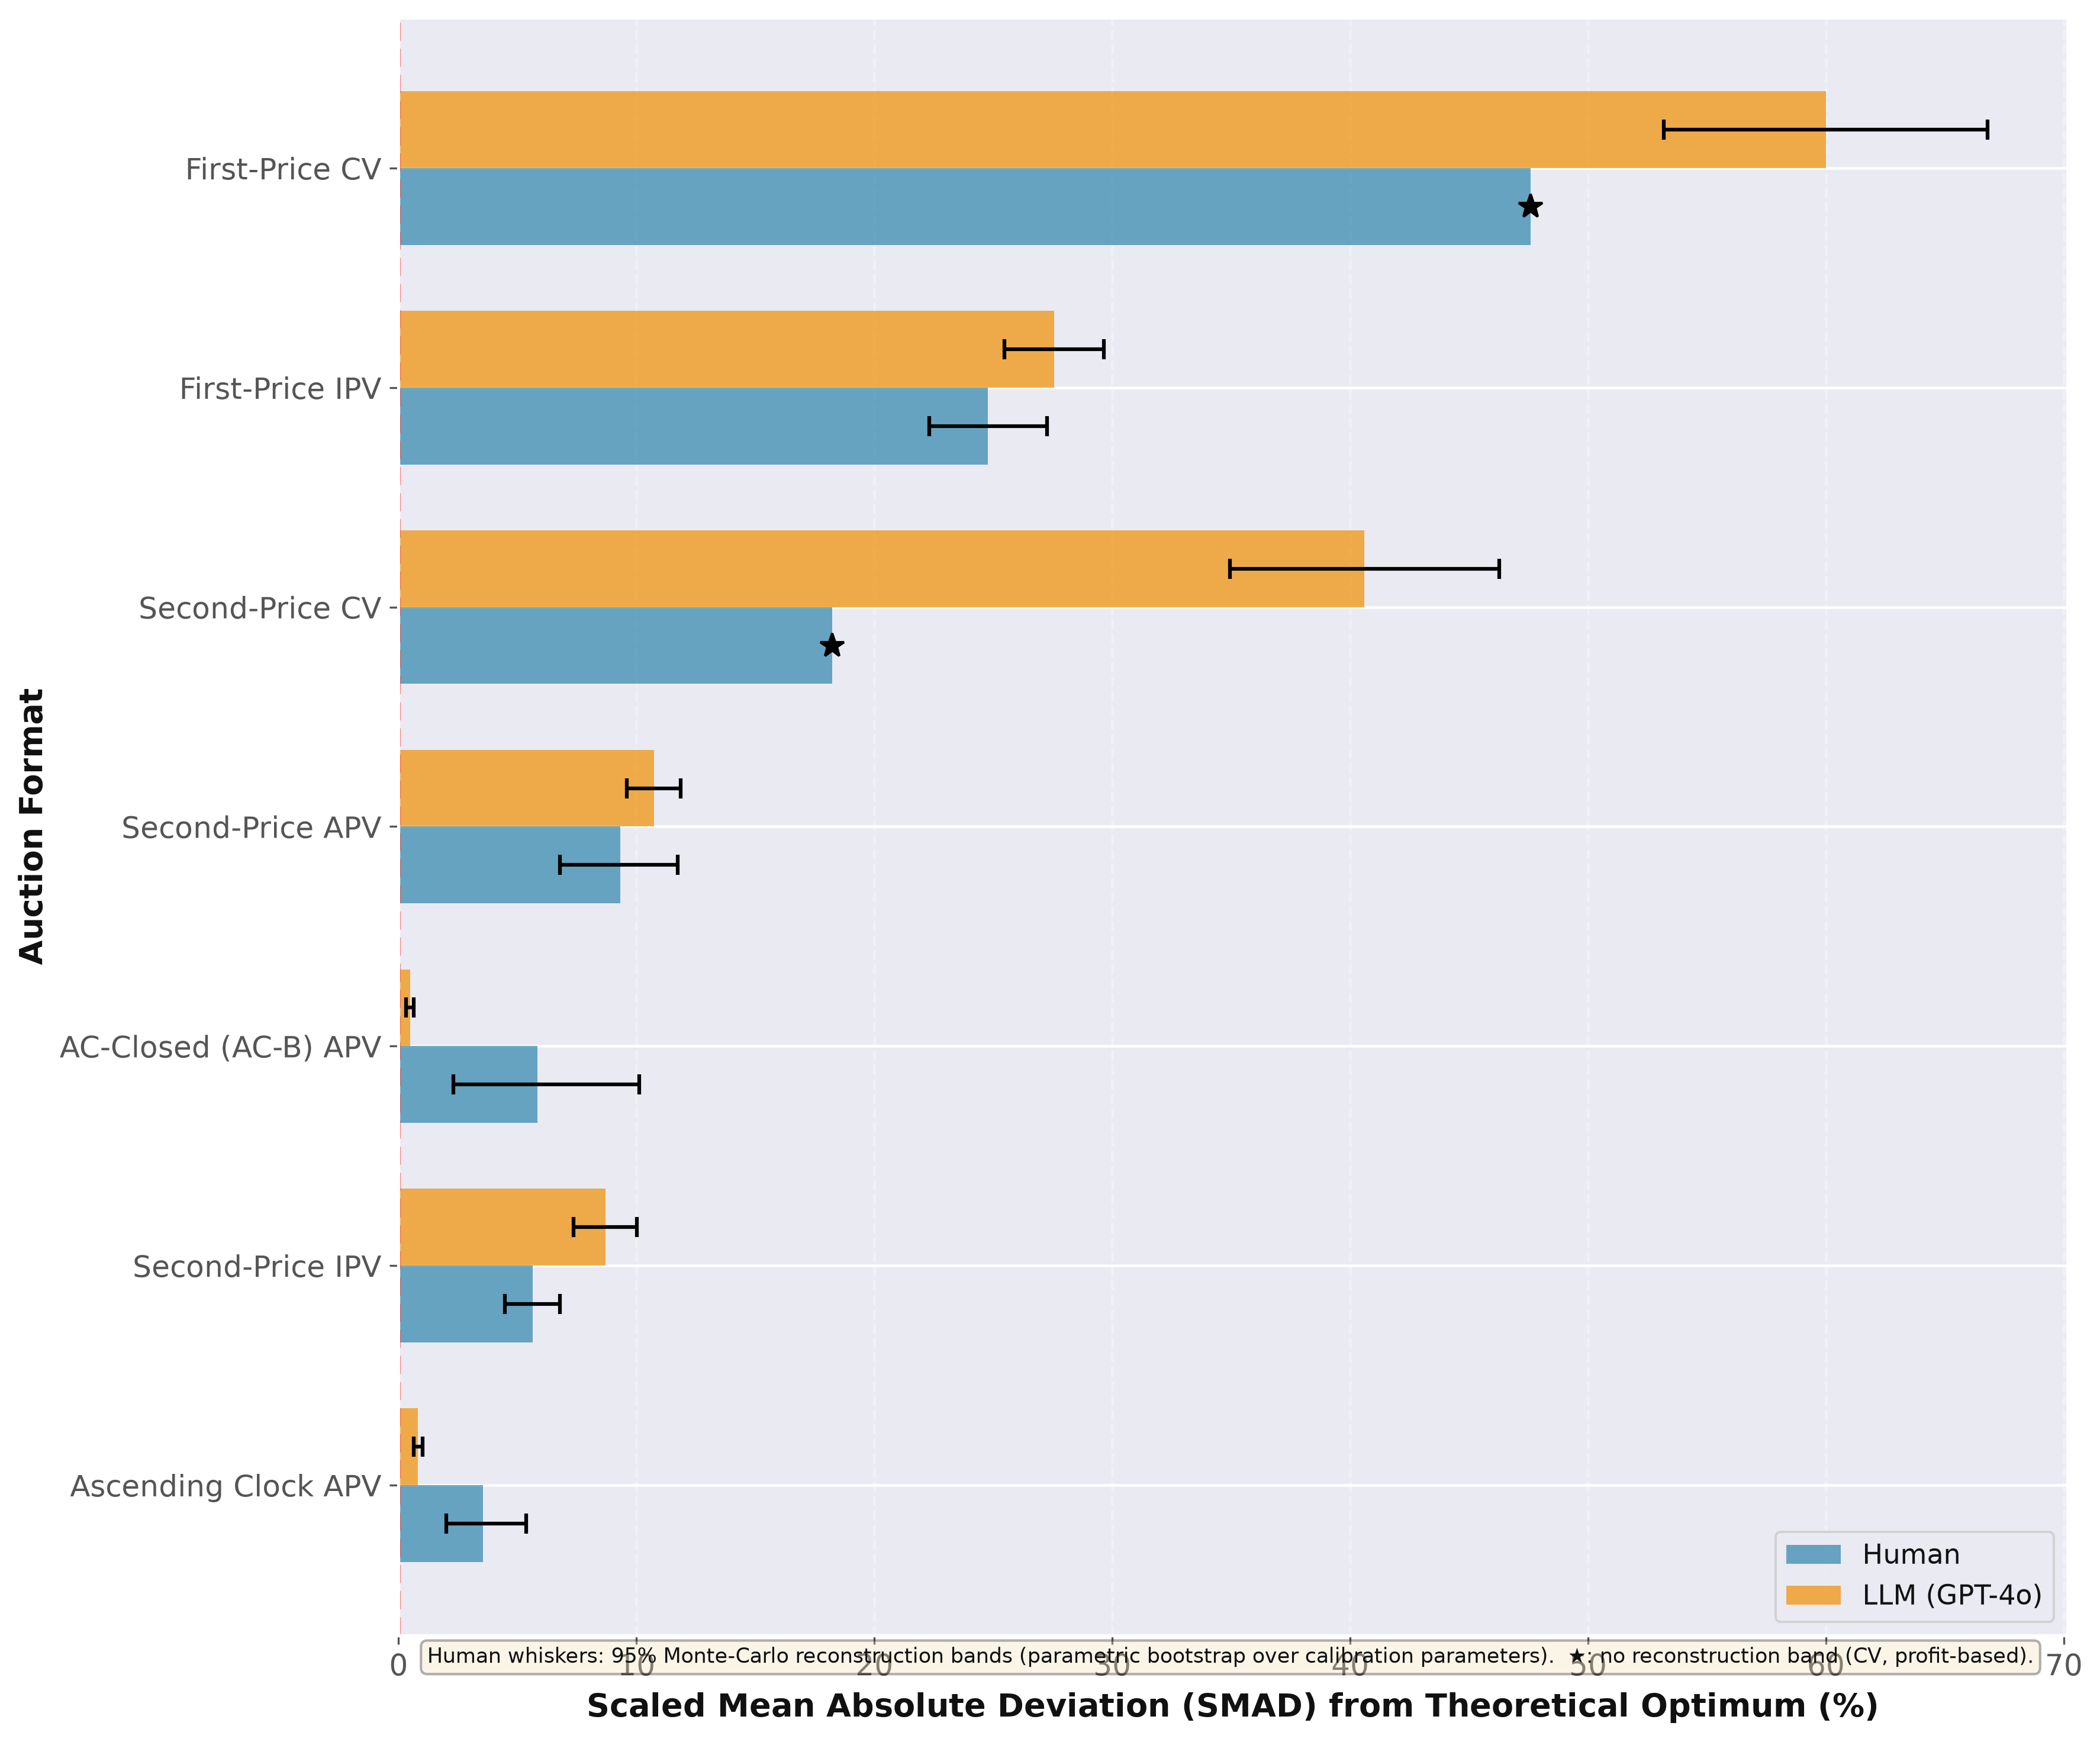
\includegraphics[width=0.82\linewidth]{figure1_bands.png}
    \caption{\textbf{Human vs.\ LLM bidding behavior across seven auction formats,
with reconstruction-uncertainty bands on the human anchors.}
Blue bars: scaled mean absolute deviation (SMAD) between human bidding and the
theoretical benchmark, computed from the moment-matched reconstructions of
Section~\ref{sec:reconstruction}. Yellow bars: SMAD between GPT-4o agents and the
same benchmark. Formats are ordered by human SMAD; LLM simulations use $N=3$
bidders. Black whiskers on the human bars are $95\%$ Monte-Carlo
reconstruction-uncertainty bands: for each source-paper calibration we re-draw
$B=2000$ vectors of the mixture parameters
$(p_{\text{eq}}, p_{\text{over}}, p_{\text{under}}, \lambda, \sigma, \delta)$
within the ranges the reported source statistics admit and propagate each draw
through the reconstruction (Appendix~\ref{app:human}). The bands are
$[22.30, 27.25]$ (FPSB IPV, point $24.76$), $[4.46, 6.79]$ (SPSB IPV, $5.65$),
$[6.78, 11.74]$ (SP-APV, $9.31$), $[2.00, 5.36]$ (AC, $3.54$), and
$[2.30, 10.11]$ (AC-B, $5.83$). The FPSB $\gg$ SPSB difficulty ordering
(ratio $95\%$ band $[3.54, 5.65]$) and the AC clock improvement over sealed SP-APV
hold in $100\%$ of the re-draws; the AC-B closed-clock improvement holds in
$92.6\%$ of re-draws, its wider band inherited from the large reported standard
error on the Breitmoser--Schweighofer-Kodritsch mean absolute deviation.
Common-value formats (marked $\star$) use a profit-based deviation metric and
carry no reconstruction band. These are calibration bands, not sampling bands on
human behavior; all comparisons remain at the level of orderings and
comparative statics (Section~\ref{sec:reconstruction}).}
    \label{fig:smad-comparison}
\end{figure}

Aggregate SMAD, however, masks a sharp divergence in \emph{how} the two populations deviate. Figure~\ref{fig:direction} decomposes errors directionally after removing near-optimal bids (within a $\pm2\%$ band of the benchmark). In the first-price IPV setting, both populations primarily \emph{overbid} relative to the risk-neutral equilibrium, but GPT-4o's overbidding is far more extreme: humans overbid $56.5\%$ of the time (with $10.4\%$ of bids near equilibrium removed), whereas GPT-4o overbids $85.9\%$ of the time and almost never lands near the benchmark ($0.7\%$ removed)---consistent with systematically more aggressive competition by LLM bidders in FPSB \citep{cox1988theory}.

The second-price IPV setting \emph{reverses direction}, and this reversal is load-bearing for the rest of the paper. Human bidders are overwhelmingly on the overbidding side: $67.2\%$ of reconstructed human bids lie strictly above value, and among bids that deviate from value at all, $92.2\%$ are overbids,\footnote{Direction shares are reported under the repository-canonical convention: the share of bids strictly above (below) value among \emph{all} bids, with the share among \emph{deviating} bids (the complement of exactly-truthful bids) in parentheses. An earlier draft reported $96.0\%$ human overbidding under a band-removal convention (deviations outside a $\pm2\%$ band of the benchmark), which Figure~\ref{fig:direction} retains; the qualitative reversal is invariant to the choice of convention.} consistent with the classic right-skewed bid distributions documented by \citet{kagel1993independent}, where most bidding mass lies above value.\footnote{In an SPSB auction with $5$ players, \citet{kagel1993independent} observed that the distribution of bids was right-skewed, with the majority of the bidding mass (67\%) representing over-bidding relative to private values. However, this figure appears inconsistent with their reported regression of bids on values; specifically, both the intercept and the coefficient exceed 1, which would typically imply a more pervasive pattern of over-bidding than the percentage suggests.} GPT-4o, by contrast, produces a predominantly \emph{left-skewed} distribution with most mass on underbidding---$74.1\%$ of bids lie strictly below value and only $16.7\%$ above ($81.6\%$ of deviating bids are underbids)---despite truthful bidding being a dominant strategy; it also places substantial probability mass at or near value ($29.2\%$ of bids within the $\pm2\%$ band of Figure~\ref{fig:direction}), reflecting a sizable fraction of exactly-truthful bids in our runs. The same reversal appears in the APV sealed-bid cell (humans $64.7\%$ overbid; GPT-4o $92.4\%$ underbid, under the figure's band convention). Humans err toward competitive overbidding under an incentive-compatible rule; GPT-4o errs toward conservatism. We record this as a declared divergence in the validity map below (Table~\ref{tab:validity-map}), and Section~\ref{sec:humans} shows why it strengthens, rather than undermines, the transferability of the lever ranking: the same design levers repair opposite-signed errors in both populations.

\begin{figure}[ht]
    \centering
    
\includegraphics[width=0.82\linewidth]{figure2_by_auction_type_10pct.png}
    \caption{\textbf{Directional decomposition of deviations, humans vs.\ GPT-4o.} Share of underbids vs.\ overbids across auction formats after removing bids within a $\pm2\%$ band of the theoretical benchmark. Humans overbid where GPT-4o underbids in the strategy-proof sealed-bid formats---the direction divergence carried into Table~\ref{tab:validity-map} and Section~\ref{sec:humans}.}
    \label{fig:direction}
\end{figure}

\subsection{The Winner's Curse in Common-Value Auctions}\label{sec:validation-curse}

Common-value auctions provide a sharp test of whether bidders correctly condition on the adverse selection implicit in winning. In the canonical design of \citet{kagel1986winner}, each bidder observes a noisy private signal $x$ about a common value $x_0$; winning is ``bad news'' because, conditional on holding the highest of $n$ signals, the expected common value lies strictly below $x$, with the gap widening in $n$.\footnote{In the standard symmetric design, $\mathbb{E}[x_0 \mid X = x_{1:n}] = x - \frac{n-1}{n+1}\varepsilon$ away from boundary regions, where $\varepsilon$ controls signal noise---competition exacerbates adverse selection.} Bidders who neglect this conditioning overbid relative to $\mathbb{E}[x_0 \mid \text{win}]$ and earn negative profits---the classic \emph{winner's curse}. The laboratory evidence delivers two comparative statics: winner losses worsen as $n$ rises (e.g., approximately $-\$1.68$ with $n=4$ versus $-\$3.68$ with $n=7$ in \citeauthor{kagel1986winner}'s benchmark conditions), and formats that reveal more information during price discovery attenuate the curse relative to first-price sealed bidding \citep{levin1996revenue}. Table~\ref{tab:winners-curse} shows that GPT-4o bidders reproduce both. In common-value FPSB auctions, winners lose money on average in every treatment, losses grow monotonically with competition (mean winner profit $-2.54$ with 4 bidders down to $-5.55$ with 7), and the share of winners earning positive profits collapses from $24\%$ to $0\%$; one-sided tests reject nonnegative winner profit in all FPSB treatments \citep{kagel1986winner}.

Under a common-value \emph{second-price} rule with the same information structure, the same comparative-static forces appear but the curse is attenuated: winners earn positive average profits with 4 bidders (mean $1.30$), roughly break even with 5, and suffer statistically significant losses only once competition is sufficiently intense ($n \ge 6$). LLM behavior thus displays a substantially stronger winner's curse in FPSB than in SPSB, mirroring the qualitative format ranking emphasized in the experimental literature \citep{levin1996revenue}.

\begin{table}[ht]
\centering
\begin{tabular}{lccccc}
\toprule
\textbf{Auction} & \textbf{Bidders} & \textbf{Mean (Std.)} & \textbf{Median} & \textbf{\% Positive} & \textbf{$p$ (Profit $<0$)} \\
\midrule
FPSB & 4 & $-2.54$ (3.87) & $-3.00$ & 24.0\% & $<0.001^{***}$ \\
FPSB & 5 & $-4.40$ (3.63) & $-4.00$ & 6.0\%  & $<0.001^{***}$ \\
FPSB & 6 & $-5.46$ (3.82) & $-5.05$ & 4.0\%  & $<0.001^{***}$ \\
FPSB & 7 & $-5.55$ (2.93) & $-5.30$ & 0.0\%  & $<0.001^{***}$ \\
\midrule
SPSB & 4 & $1.30$ (4.87)  & $1.00$  & 58.0\% & 0.967 \\
SPSB & 5 & $0.07$ (4.35)  & $0.00$  & 46.0\% & 0.542 \\
SPSB & 6 & $-2.82$ (3.50) & $-1.75$ & 18.0\% & $<0.001^{***}$ \\
SPSB & 7 & $-2.83$ (2.78) & $-2.00$ & 12.0\% & $<0.001^{***}$ \\
\bottomrule
\end{tabular}
\caption{Winner profit in common-value auctions with GPT-4o bidders. The last column reports one-sided $p$-values for the hypothesis that winner profit is negative. *** denotes $p < 0.001$.}
\label{tab:winners-curse}
\end{table}

\subsection{Stability}\label{sec:validation-stability}

Two ablations establish that the behaviors above are stable properties of the agents rather than artifacts of run structure or decoding noise. First, in a multi-round ablation with full history feedback, GPT-4o shows no cross-round learning over 15 rounds: mean FPSB SMAD is $0.2523$ in the first five rounds versus $0.2524$ in the last five ($t$-test $p = 0.997$; Mann--Whitney $p = 0.913$), with the SPSB comparison likewise null ($0.1282$ vs.\ $0.1447$, n.s.), and trend tests detect no drift (Appendix~\ref{app:learning}). This justifies the one-shot design used throughout and implies that the lever effects in Section~\ref{sec:ranking} cannot be attributed to within-session adaptation. Second, sampling-temperature effects on deviations are modest and non-monotonic across formats; $T=0.5$ is retained as a convention for comparability rather than for performance, and model-tier ablations (a frontier reasoning model and a capability floor) are reported alongside (Appendix~\ref{app:ablations}).

\subsection{A Validity Map}\label{sec:validation-map}

Table~\ref{tab:validity-map} collects the section's evidence into an explicit accounting of what transfers from human populations to LLM agents and what does not. Four phenomena transfer: the cross-mechanism difficulty ordering, the clock/OSP format effect, the winner's-curse comparative statics, and---on average across models---the menu-description null, though the menu case transfers with a caveat: the average effect is null, but individual models shift in both directions (Section~\ref{sec:ranking-descriptions}). Two phenomena do not transfer, and we declare them as the map's red cells: the \emph{direction} of deviations under strategy-proof sealed-bid rules (humans overbid; GPT-4o underbids) and the \emph{levels and distributional shape} of deviations (LLMs place a point mass at exactly truthful play that humans lack, and levels are not calibrated across populations).

\begin{table}[!htbp]
\centering
\small
\begin{tabularx}{\textwidth}{>{\raggedright\arraybackslash}p{2.55cm} >{\raggedright\arraybackslash}X >{\raggedright\arraybackslash}X >{\raggedright\arraybackslash}p{1.75cm}}
\toprule
\textbf{Phenomenon} & \textbf{Human finding} & \textbf{LLM finding} & \textbf{Verdict} \\
\midrule
Cross-mechanism difficulty ranking & FPSB $\gg$ SPSB in SMAD (24.76\% vs.\ 5.65\%); harder formats harder everywhere & Same ordering (27.55\% vs.\ 8.69\%); ordering preserved across the battery (Fig.~\ref{fig:smad-comparison}) & Transfers ($\checkmark$) \\
\addlinespace
Clock/OSP format effect & Clock formats reduce deviations vs.\ sealed SPSB-APV: 3.54\% (AC), 5.83\% (AC-B) vs.\ 9.31\% \citep{li2017obviously,breitmoser2022obviousness} & Same direction, larger effect: 0.81\% (AC), 0.47\% (AC-B) vs.\ 10.73\% (Section~\ref{sec:ranking-extensive}) & Transfers ($\checkmark$) \\
\addlinespace
Winner's-curse comparative statics & CV-FPSB winner losses grow with $n$; attenuated under formats revealing more information \citep{kagel1986winner,levin1996revenue} & Mean winner profit $-2.54 \to -5.55$ as $n{:}\,4 \to 7$; \% positive $24\% \to 0\%$; SPSB attenuated (Table~\ref{tab:winners-curse}) & Transfers ($\checkmark$) \\
\addlinespace
Menu-description null & Menu restatement of SPSB leaves human bidding essentially unchanged \citep{gonczarowski2023strategyproofness} & Small and sign-mixed across the four models: null on average (placebo sign test $p=0.73$); slightly worse for Claude ($p=0.042$) and GPT-4o ($p=0.003$), null for Gemma ($p=0.94$), better for Gemini ($p<0.001$) (Section~\ref{sec:ranking-descriptions}) & Transfers on average ($\checkmark$), heterogeneous \\
\addlinespace
Deviation \emph{direction} (strategy-proof sealed bid) & Overbidding: 67.2\% of bids above value; 92.2\% of deviating bids (SPSB-IPV); 64.7\% of out-of-band deviations (APV) & Underbidding: 74.1\% of bids below value; 81.6\% of deviating bids (SPSB-IPV); 92.4\% (APV, band convention) & Diverges ($\times$) \\
\addlinespace
Deviation \emph{levels} and shape & Continuous, right-skewed bid distributions; little mass exactly at value & Point mass at truthful play (29.2\% within $\pm2\%$ in SPSB-IPV; 71.7\% in AC vs.\ 26.8\% for humans); levels not calibrated across populations & Diverges ($\times$) \\
\bottomrule
\end{tabularx}
\caption{\textbf{Validity map: which behavioral phenomena transfer from human experimental populations to LLM agents.} Human findings are from the cited experimental and field literatures via the moment-matched reconstructions of Section~\ref{sec:reconstruction}; LLM findings are from this section and Section~\ref{sec:ranking}. Verdicts are qualitative: transfers = same sign and comparative statics; diverges = opposite sign or uncalibrated levels. \TODO{Add a rank-concordance statistic with a bootstrap CI to the difficulty-ordering row (residual of E6; the other transferring rows now carry cell-level tests).}}
\label{tab:validity-map}
\end{table}

The two red cells discipline everything that follows. Because deviation levels and directions do not transfer, the ranking in Section~\ref{sec:ranking} is never built on cross-population level comparisons: every lever is scored by the preservation index $\rho$, a within-model ratio to that model's own baseline, which is invariant to both the sign and the scale of a population's characteristic error. And because transfer cannot be assumed, Section~\ref{sec:humans} treats it explicitly, anchoring each rung of the ranking to human evidence where it exists---where, as the map's transferring rows already suggest, the levers move both populations in the same direction even when their baseline errors point opposite ways.

% ============================================================================
% 06_ranking.tex — Section 6: The Simplicity-Preservation Ranking
% Rewrite pass (2026-07): auctions are the main domain; DA is the robustness/
% generalization domain (Appendix app:da; landing owned by the appendix
% writer). All numbers wired to the merged seed-1299 datasets:
% results/merged_ranking/{auction_cells.csv,da_cells.csv,concordance.md} and
% results/traces/{traces_summary.md,traces_subsection.tex}. E3 menu and
% clock-framing cells are four-model; tab:ranking carries pooled rho medians
% with double-bootstrap 95% CIs; fig:ranking = ranking_forest.pdf (real);
% fig:ranking-framing = figure3_intervention_comparison.png (real, 2x4);
% new subsection sec:ranking-traces (+ tab:trace-dissociation).
% NOTE for integrator: clock-framing (B3) = the intervention_proxy_breitmoser
% sealed-bid cells (SMAD 6.3-13.8%, pooled rho +0.29); the SMAD 1.4-5.2%,
% p<0.001-all-four, d-up-to-1.00 cells are the TRUE closed clock
% (ascending_clock_closed, family A), per concordance.md and the R6 audit in
% appendix_prompts. The two rungs are reported separately below.
% ============================================================================

\section{The Simplicity-Preservation Ranking}\label{sec:ranking}

This section delivers the paper's central product: an empirical ranking of the
design levers of Section~\ref{sec:framework} by how well each preserves
dominant-strategy play. Auctions are the domain throughout; one lever---the
menu description---is additionally probed in a supplementary school-choice
matching experiment (deferred acceptance) reported in
Appendix~\ref{app:da}, drawn on below where it sharpens the descriptions
result. We proceed in three passes over the
lever taxonomy. Section~\ref{sec:ranking-extensive} evaluates the
extensive-form lever (family~A): replacing the sealed-bid auction with an
ascending clock. This is the lever for which simplicity theory makes its
sharpest predictions, and it sits at the top of the ranking---but it bundles
several simplifications at once. Sections~\ref{sec:ranking-descriptions}
and~\ref{sec:ranking-scaffolds} therefore decompose the bundle with
presentation-only levers that hold the extensive form fixed: descriptions of
the mechanism (family~B) and reasoning scaffolds appended to it (family~C).
Section~\ref{sec:ranking-synthesis} assembles the cells into the ranking
itself (Table~\ref{tab:ranking} and Figure~\ref{fig:ranking}), and
Section~\ref{sec:ranking-traces} closes the section by reading the agents'
own stated reasoning against their realized bids.

Throughout, $D(L,m)$ denotes the deviation of model $m$ from
dominant-strategy play under lever $L$: the mean
bid deviation from value (bid $-$ value, in dollars), with the scaled mean
absolute deviation (SMAD; normalizer $E[b^{*}] = \$24.5$,
Section~\ref{sec:metrics}) reported in parallel. Every cell-level statistic
below---bootstrap confidence intervals (2{,}000 draws, seed 1299),
Mann--Whitney and Welch tests, Cohen's $d$---is computed from the merged
run-level dataset in the replication package
(\path{results/merged_ranking/auction_cells.csv}). Two auction baseline conventions
appear in what follows, and we fix them here once. \emph{Format-level}
comparisons (sealed bid vs.\ clock) use the dedicated SPSB cells, with
per-model mean deviations of $-0.49$ (Claude), $-1.63$ (Gemini), $-3.28$
(GPT-4o), and $-5.27$ (Gemma)---cross-model mean $-\$2.67$.
\emph{Presentation and scaffold} contrasts are tested against the pooled
axis baselines run in the same grid as each treatment---with one correction
made in this draft: a provenance audit showed that the legacy ``axis-2
baseline'' cell was itself a treated clock-framing description
(Section~\ref{sec:ranking-synthesis}), so the pool comprises the axis-1 and
axis-3 baseline cells only, with per-model means of $+0.54$ (Claude),
$-1.25$ (Gemini), $-2.94$ (GPT-4o), and $-6.53$ (Gemma)---cross-model
$-\$2.55$. The two conventions differ materially for Claude, Gemini, and
Gemma, and both are recorded cell by cell in the replication file. The comparative statistic is the preservation index
$\rho$ of Section~\ref{sec:metrics}, computed within model on
the absolute-deviation scale and pooled as the median across cells:
$\rho = 1$ is perfect preservation of dominant-strategy play, $\rho = 0$ no
effect, and $\rho < 0$ a lever that \emph{backfires}. Because $\rho$ is
computed within model, the ranking is invariant to cross-model differences in
baseline levels.

\subsection{Extensive-Form Levers: The Ascending Clock}
\label{sec:ranking-extensive}

A strategy-proof mechanism and its OSP counterpart implement the same outcome
rule---the same mapping from reports to allocations and payments---but differ
in extensive form. The non-OSP version requires \emph{contingent reasoning}:
to see that truth-telling is dominant, an agent must trace through
hypothetical scenarios about others' behavior and verify that no deviation
improves payoffs in any case. The OSP version restructures the game so that
the dominant strategy is \emph{obviously} optimal: at every information set,
the best outcome from following the strategy weakly dominates the worst
outcome from any deviation, without requiring any reasoning about what others
might do \citep{li2017obviously}. Section~\ref{sec:validation} established
that LLM agents deviate from truthful play in sealed-bid strategy-proof
formats. Here we ask how much of that deviation the extensive form itself
removes, across all four model families.

\begin{figure}[htbp]
    \centering
    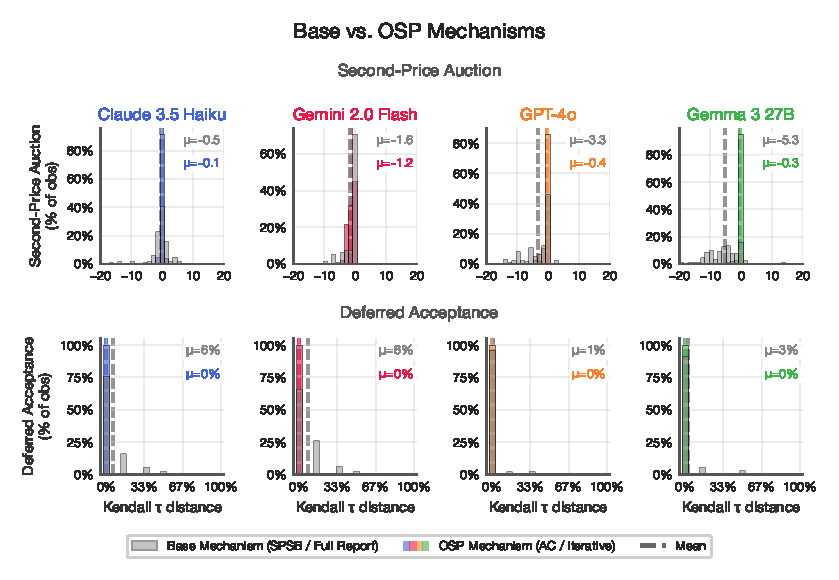
\includegraphics[width=\textwidth]{fig1_osp_comparison.pdf}
    \caption{Comparing base (non-OSP) and OSP mechanisms across four model
    families. Distribution of bid
    deviations from value ($\text{bid} - \text{value}$) in second-price
    sealed-bid (gray) and ascending clock (colored) auctions. Dashed lines
    indicate means. All models deviate from truthful
    play in the non-OSP sealed-bid format; the ascending clock corrects toward
    truth-telling.}
    \label{fig:osp-comparison}
\end{figure}

\paragraph{The human-anchored APV cell.}
Clock auctions are dynamic formats in which the price rises incrementally and
bidders decide whether to stay in or drop out at each price point. Although
the sealed-bid second-price format and the ascending clock share the same
dominant strategy, human participants behave quite differently across them: a
robust pattern in the experimental literature is that bidders do much better
in clock-style auctions than in sealed-bid auctions. \citet{li2017obviously}
provides an argument for why clock auctions are easier to recognize as
strategy-proof, formalized as obvious strategy-proofness, and
\citet{breitmoser2022obviousness} provide additional evidence that clock
auctions improve truthful play, with behavior under the open clock (AC, where
dropouts are observed) slightly better than under the closed clock (AC-B).

We evaluate the clock lever in two purpose-labeled cells
(Table~\ref{tab:calibration-master}). The first is an affiliated private
values (APV) environment chosen for comparability with the human evidence of
\citet{li2017obviously} and \citet{breitmoser2022obviousness}. While
affiliation could in principle change incentives through correlation in
values, the three formats we consider are strategically equivalent: in the
second-price sealed-bid (SP), the open ascending clock (AC), and the closed
clock (AC-B), it remains a dominant strategy to bid---or drop out at---one's
value. Reconstructed human bidders deviate substantially less from truthful
bidding in the clock formats than in sealed-bid SP: SMAD is $3.54\%$ in AC and
$5.83\%$ in AC-B, compared to $9.31\%$ in SP
(Figure~\ref{fig:smad-comparison}). For GPT-4o the clock advantage is even
more pronounced. In the APV clock auctions GPT-4o achieves near-truthful play,
with SMAD falling to $0.81\%$ in AC and $0.47\%$ in AC-B (a $77\%$--$92\%$
reduction relative to the human clock baselines), whereas in sealed-bid SP it
remains at $10.73\%$---close to the human level of $9.31\%$. Breaking the
decision into a sequence of simple threshold choices (``stay iff the price is
below value'') yields an order-of-magnitude improvement over the one-shot
sealed-bid interface, even though the dominant-strategy benchmark is
identical.

The direction of the residual mistakes matters as much as their size.
Figure~\ref{fig:direction} decomposes bidding errors by direction using a
$\pm 2\%$ tolerance band around value (dropping near-equal bids and
classifying the remainder as under- vs.\ over-bids). Despite comparable
aggregate deviations in sealed-bid SP-APV ($9.31\%$ vs.\ $10.73\%$ SMAD), the
nature of the deviations differs strikingly: human bids are predominantly
\emph{above} value ($64.7\%$ overbidding vs.\ $35.3\%$ underbidding), while
GPT-4o bids are predominantly \emph{below} value ($92.4\%$ underbidding vs.\
$7.6\%$ overbidding)---humans exhibit competitive overbidding even under an
incentive-compatible rule, while GPT-4o is overly conservative in the
sealed-bid interface. The clock aligns not only the magnitude but the
\emph{shape} of behavior: in AC, humans and GPT-4o display an almost perfectly
symmetric under/over split ($49.2/50.8$ vs.\ $50/50$), with GPT-4o
concentrating far more mass near truthful bidding ($71.7\%$ within $\pm 2\%$
vs.\ $26.8\%$ for humans). We return to what this direction reversal does---%
and does not---imply for the ranking in Section~\ref{sec:humans}.

\paragraph{The four-model IPV cell.}
The second cell runs the same lever in the independent private values (IPV)
environment of Table~\ref{tab:calibration-master}, across all four model
families; its purpose is identification rather than human comparability.
In the SPSB baseline (Figure~\ref{fig:osp-comparison}, left column, gray), all
four models deviate from truthful bidding, with mean deviations of
$\mu = -0.49$ (Claude), $-1.63$ (Gemini), $-3.28$ (GPT-4o), and $-5.27$
(Gemma), for a cross-model mean of $-\$2.67$; these are the dedicated SPSB
cells of the baseline declaration above. The negative sign indicates
systematic \emph{underbidding}---the mirror image of the human overbidding
documented in Section~\ref{sec:validation}. The distributions also exhibit
long tails: some bids deviate by \$10--20 from value, cases in which the
model substantially misplays the auction.

The closed ascending clock corrects deviations toward truthful play in every
model. Mean deviations compress to $\mu = -0.05$ (Claude), $-1.24$ (Gemini),
$-0.45$ (GPT-4o), and $-0.33$ (Gemma)---a cross-model mean of roughly
$-\$0.5$---and SMAD falls to $1.4\%$, $5.2\%$, $1.9\%$, and $1.9\%$ against
pooled-axis baselines of $9.5\%$, $11.7\%$, $11.4\%$, and $20.7\%$. The shift
is significant for every model (Welch $p < 0.001$ in all four cells), with
effect sizes up to Cohen's $d = 1.00$ (Gemma). The improvement is most
dramatic for the models with the worst SPSB performance: Gemma's mean
deviation falls from $-5.27$ to $-0.33$, a near-complete correction. Beyond
the mean shifts, the clock \emph{eliminates the long tails} visible in the
SPSB distributions: the catastrophic deviations effectively disappear. This
variance reduction may be as practically important as the mean
correction---OSP does not merely improve average play, it also removes the
worst-case failures. Because this cell is run under IPV, the improvement
cannot be informational.\footnote{In a common- or affiliated-values setting,
the clock format could improve play by revealing information about others'
values through their dropout decisions. Under IPV, no such information
exists, so the improvement must be purely cognitive.}
Two provenance notes complete this cell's accounting. The environment audit
(plan E2) found that the legacy \path{ascending_clock_closed} runs pair an
affiliated-values \emph{description} with independent private-value
\emph{draws} (the configuration's value model sets the common component to
zero), so the informational channel was already absent in the data---but the
prompt and the environment disagreed. A dedicated clean IPV cell
(\path{ascending_clock_ipv_closed}: IPV description, IPV draws, $\$0.5$
tick, seed 1299, $K = 50$) now exists for GPT-4o and Gemma and reproduces
the result exactly---SMAD $1.5\%$ (GPT-4o) and $1.8\%$ (Gemma) against
sealed baselines of $12$--$27\%$---so the identification claim does not rest
on the mislabeled cells. The remaining IPV-clock cells for Claude 3.5 Haiku and Gemini
2.0 Flash await native-API access (both model snapshots have been retired
from the aggregator used for this draft's re-runs); given the exact
replication in the two available families and the direction of every legacy
cell, we do not expect the remaining two cells to change the rung.

\paragraph{The bridge: which margin does the work?}
In summary, LLMs deviate from dominant-strategy play in the sealed-bid
strategy-proof auction, and the OSP ascending clock substantially corrects these
deviations. As a design lesson, however, the extensive-form result is coarse,
because OSP changes several things at once: it changes the game tree, it
coarsens the action space to simple binary or menu choices, and it makes the
safety property of truth-telling salient at every decision point. The clock
eliminates the need for contingent reasoning, reduces each decision to a
stay/exit choice, and makes the connection between action and outcome
immediate. Which of these simplifications actually drives the improvement?
The theory does not need to answer this question---any OSP implementation
bundles them---but a designer does, because the margins have very different
costs: re-engineering the extensive form of a deployed mechanism is
expensive, while changing its description, or the reasoning it invites, is
nearly free. The next two subsections decompose the bundle with
presentation-only levers that hold the sealed-bid extensive form fixed:
descriptions of the mechanism (family~B,
Section~\ref{sec:ranking-descriptions}) and reasoning scaffolds appended to
it (family~C, Section~\ref{sec:ranking-scaffolds}).

\subsection{Descriptions: Restating the Rules versus Exposing the Safety
Invariant}\label{sec:ranking-descriptions}

Family~B holds the mechanism fixed and varies only how it is described.
Recent studies ask whether behavior in strategy-proof mechanisms depends on
how the mechanism is \emph{presented}, holding the underlying incentives
fixed. \citet{gonczarowski2023strategyproofness} propose
strategyproofness-exposing descriptions, including an extensive-form
\emph{menu} description that compresses the dominant-strategy logic of a
second-price auction into a short menu statement intended to make
strategy-proofness salient; in their laboratory experiments, however, this
menu framing does not meaningfully change human bidding relative to the
traditional SPSB description, and \citet{gonczarowski2024describing} likewise
find that menu-based explanations of DA improve measured \emph{understanding}
while average behavioral effects remain modest. In contrast,
\citet{breitmoser2022obviousness} show that \emph{reframing} SPSB as a
dynamic ascending clock substantially increases truthful play by human
subjects. The taxonomy of Section~\ref{sec:framework} accordingly splits the
family into three sub-levers---menu restatement (B1), safety-exposing
descriptions (B2), and clock-framing (B3)---and they turn out to behave very
differently.

\paragraph{Menu restatement (B1): null on average, sign-mixed underneath.}
The menu restatement has no consistent effect on bidding. Across the four
models, its effects are small and sign-mixed relative to each model's pooled
axis baseline (Figure~\ref{fig:ranking-framing}, top row): Gemma is a clean
null (mean deviation $-4.50$ vs.\ baseline $-4.54$; Welch $p = 0.94$), Claude
moves slightly \emph{away} from truthful play ($+0.48$ to $+1.37$,
$\Delta = +0.88$ above value, $p = 0.042$, $d = 0.24$), GPT-4o moves
\emph{away} as well ($-2.78$ to $-4.10$, $\Delta = -1.32$, $p = 0.003$,
$d = -0.37$), and Gemini alone moves \emph{toward} truthful bidding ($-2.88$
to $-1.13$, $\Delta = +1.75$, $p < 0.001$, $d = 0.50$). Pooling across cells,
the restatement is a null on average: a two-sided sign test of the B1 cells
against their baselines cannot reject no effect ($p = 0.73$;
Section~\ref{sec:ranking-synthesis}). The pattern also survives payment-rule
variation: in GPT-4o's first- and third-price variants of the same grid, the
menu cells are indistinguishable from their baselines ($p = 0.63$ and
$0.51$). We therefore read the menu cell as consistent with the human
null \emph{on average} \citep{gonczarowski2023strategyproofness,
gonczarowski2024describing}, with the caveat that the average conceals
genuine model-level heterogeneity---a point the human experiments, run on a
single population, cannot speak to. The menu family turns out to be more
interesting in the supplementary matching experiment, where it splits into two
sub-variants with opposite effects; we return to this in
Section~\ref{sec:ranking-synthesis}.

\paragraph{Clock-framing (B3): describing the bid as a clock exit.}
The clock-framing description keeps the one-shot sealed-bid elicitation---the
agent still submits a single number---but describes that number as the
threshold at which an automatic proxy would exit an ascending clock on the
bidder's behalf. This is a description, not a mechanism change: no prices are
posted, no dropouts occur, and no information is revealed; it should not be
conflated with the AC/AC-B formats of Section~\ref{sec:ranking-extensive}.
The two rungs are empirically distinct cells in the merged dataset: the
clock-framing cells record exactly one sealed bid per bidder per auction,
while the true clock cells record per-tick stay/exit decisions
(Appendix~\ref{app:prompts}). Against the corrected pooled baselines
(Section~\ref{sec:ranking-synthesis}), clock-framing moves play
significantly in every model family but not always in the same direction
(Figure~\ref{fig:ranking-framing}, bottom row): SMAD falls from $12.1\%$ to
$6.3\%$ for GPT-4o and from $26.8\%$ to $13.8\%$ for Gemma---each
roughly halving its deviation---and from $8.3\%$ to $7.2\%$ for Claude (all
Welch $p < 0.001$), while Gemini moves the \emph{wrong} way, from $5.1\%$ to
$9.5\%$ ($p < 0.001$). The sign agrees with the human evidence that clock
reframing increases truthful play \citep{breitmoser2022obviousness} in three
of the four families, and the exception is coherent rather than noisy:
Gemini is also the one model that the two-stage clock-exit variant below
sharply harms. Pooled, the rung is modest and dispersed---median
$\rho = +0.30$ ($95\%$ CI $[-0.77, +0.52]$, the width driven by the Gemini
reversal)---recovering, where it works, a third to a half of the gap to
truthful play, where the true extensive-form clock recovers nearly all of it
(SMAD $1.4$--$5.2\%$; Section~\ref{sec:ranking-extensive}). Words that
borrow the clock's framing can help, and for some models help substantially;
the clock itself helps every model, and helps far more.

The rung comes with a measured warning about paraphrase sensitivity. A
provenance audit of the legacy run grid (documented in the replication
package) uncovered a \emph{second} clock-framing text that had been
mislabeled as an axis-2 baseline cell: a two-stage description that presents
the sealed bid as an ``exit price'' at which an ascending price clock would
remove the bidder. Its manipulation check passes---clock-and-exit language
appears in $14.3\%$ of treated traces against $0\%$ in the corrected
baselines (wild-cluster $p = 0.002$)---but its behavioral effects, unlike
the canonical clock-framing text above, are violently heterogeneous: it
nearly fixes Gemma (mean deviation $-6.53$ to $-0.59$), sharply
\emph{backfires} for Gemini ($-1.25$ to $-6.12$), and leaves Claude and
GPT-4o unmoved, with GPT-4o inert in language as well as bids (zero echo of
the framing), so that the pooled effect is a null that conceals offsetting
model-level responses ($p = 0.88$ pooled). The two texts agree on one
regularity---both harm Gemini, the family most reactive to clock
vocabulary---but otherwise produce different model-level profiles from the
same clock analogy: the canonical framing helps three families, the
two-stage variant helps only Gemma. This is direct evidence that
description effects are sensitive to wording in a way that extensive-form
changes are not (the true clock helps every model; Section~%
\ref{sec:ranking-extensive}), and a caution against reading any single
description cell, including ours, as \emph{the} effect of its family.

\paragraph{Safety-exposing descriptions (B2): stating the invariant.}
The safety-exposing sub-family does not restate the rules at all; it states
the structural property of the mechanism that makes truth-telling safe. The
key step in \citet{vickrey1961counterspeculation}'s original argument for the
strategy-proofness of the second-price auction concerns being
\emph{pivotal}: your bid determines only \emph{that} you win, not \emph{what}
you pay. This inspires our \emph{Payoff Safety} intervention for the auction
setting: ``Think of your bid as setting your maximum price. Your bid
determines IF you win, not WHAT you pay. If you win, you pay what others bid,
not what you bid.'' Its analogue in the supplementary matching experiment, \emph{Rejection
Safety}, states the property that made deferred acceptance preferable to the
Boston mechanism in practice \citep{abdulkadirouglu2003school}: ``Rejections
only redirect, never eliminate. Your ranking determines the \emph{order} in
which you are considered, not \emph{whether} you are considered.'' Neither
intervention scaffolds a particular mode of reasoning: they do not ask the
agent to trace through contingencies, simulate the algorithm, or reason about
opponents. They simply state the key property of the mechanism that makes it
strategy-proof.

In auctions, \emph{Payoff Safety} reduces the mean deviation from
$\mu = -2.67$ to $-1.53$ (Figure~\ref{fig:descriptions}), with the deviation
shrinking in magnitude for every model: Claude from $-0.49$ to $+0.30$,
Gemini from $-1.63$ to $-0.38$, GPT-4o from $-3.28$ to $-1.88$, and Gemma
from $-5.27$ to $-4.17$.\footnote{The Claude endpoint is $+0.30$
(overbidding) in the raw logs; the ES manuscript reported it as $-0.30$. The
magnitude is identical and the qualitative claim---Claude ends closest to
truthful---is unchanged, but the sign correction means Claude's residual
error flips from under- to over-bidding under this description.} Against the
axis-specific baselines the improvement is significant for Gemini
($p < 10^{-30}$, $d = 1.85$) and GPT-4o (Mann--Whitney $p < 10^{-5}$); for
Claude the mean effect is null while dispersion halves (SMAD $12.0\%$ to
$4.8\%$); Gemma is the one negative mark, moving away from its axis-2
baseline---though that baseline is anomalously low relative to Gemma's other
baselines, a caveat we quantify in Section~\ref{sec:ranking-synthesis}. For
comparison, the ascending clock achieves $\mu \approx -0.5$
(Section~\ref{sec:ranking-extensive}); the description closes roughly half
the gap.

That a brief description of a mechanism's incentive properties can nearly
replicate OSP's effect---without changing the extensive form---is a
surprising result. It suggests that the cognitive barrier for LLMs in non-OSP
mechanisms is not in \emph{computing} the dominant strategy given the game
tree, but in understanding the mechanism well enough to \emph{see that
truth-telling is safe}. OSP mechanisms resolve both problems simultaneously:
they simplify the game tree and make the safety guarantee transparent. Our
results suggest it is the latter that does most of the work, at least for
LLMs.

Descriptions, then, are two levers, not one---and the split is not between
``more text'' and ``less text'' but between what the text \emph{asserts}.
Restating the rules, even in the theoretically grounded menu form, is null on
average and sign-mixed underneath; exposing the safety invariant recovers
most of what full OSP implementation delivers, in every model whose baseline
leaves room to improve. The menu cell still functions as a placebo in the
aggregate---not every additional sentence about the mechanism moves behavior,
so the large effects of B2 cannot be attributed to generic prompt
sensitivity---but it is a noisier placebo than a single-population experiment
would suggest. What the effective descriptions share, and the restatement
lacks, is that they \emph{assert} the invariant that makes truth-telling safe
rather than leaving the agent to derive it. The supplementary matching
experiment sharpens this reading to a within-family contrast, discussed in
Section~\ref{sec:ranking-synthesis}: a menu description that adds the
invariance statement behaves like a safety description, while a menu
description that merely restates the computation backfires.

\begin{figure}[htbp]
    \centering
    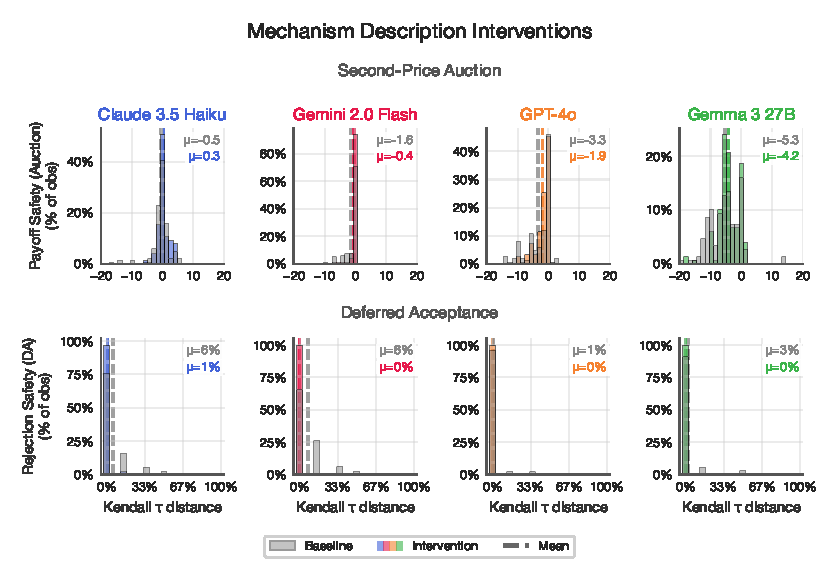
\includegraphics[width=\textwidth]{fig5_mechanism_description.pdf}
    \caption{Safety-exposing description (B2): \emph{Payoff Safety} in
    second-price auctions (``your bid determines IF you win, not WHAT you
    pay''), across the four model families. Baseline in
    gray, intervention in color; dashed lines indicate means. The intervention
    improves play in every model, closing roughly half the gap to the full OSP
    result of Figure~\ref{fig:osp-comparison}.}
    \label{fig:descriptions}
\end{figure}

\begin{figure}[htbp]
    \centering
    
\includegraphics[width=0.9\linewidth]{figure3_intervention_comparison.png}
    \caption{Presentation-only descriptions of the same SPSB mechanism,
    across all four model families ($2 \times 4$ panels; deviations in
    dollars). \emph{Top row:} menu restatement (B1) vs.\ the pooled axis
    baseline---small, sign-mixed shifts (Gemma null, Claude and GPT-4o
    slightly away from truthful play, Gemini toward it). \emph{Bottom row:}
    clock-framing (B3)---a same-signed improvement in every model,
    significant in three of four. Only LLM simulation data are shown.}
    \label{fig:ranking-framing}
\end{figure}

\subsection{Reasoning Scaffolds: Contingencies Help, Strategizing Hurts}
\label{sec:ranking-scaffolds}

Family~C holds both the mechanism and its rule description fixed and appends
a reasoning scaffold. Following \citet{li2024designing}, who decomposes the
cognitive demands of mechanisms into three dimensions, we scaffold thinking
\emph{contingently} about unobserved moves by other players (C1),
\emph{planning} for one's own future moves (C2), and reasoning about other
players' \emph{beliefs} (C3). Each scaffold directs reasoning without
revealing the dominant strategy; each modifies only the rule-explanation
block of the prompt while the mechanism, value distributions, and response
format are unchanged (full prompt texts in Appendix~\ref{app:prompts}).
Prospect-theory-inspired preference framings (family~D) are reported in
Appendix~\ref{app:prospect}; they form the ranking's bottom rungs.

\subsubsection{Contingent reasoning (C1): the payoff tree}
\label{sec:ranking-contingent}

\citet{li2024designing} identifies contingent reasoning as the core cognitive
demand of non-OSP mechanisms. To see that truth-telling is dominant in SPSB,
a bidder must consider each possible profile of opponent bids and check that
no deviation improves payoffs in any case---a ``case-by-case comparison,
calculating payoffs for each profile of opponent bids''
\citep{li2024designing}. The ascending clock eliminates this demand: at each
price, the worst case from following the dominant strategy weakly dominates
the best case from any deviation, without reference to opponents. The
question is whether scaffolding contingent reasoning---without changing the
extensive form---can partially recover these gains. Our \emph{Payoff Tree}
intervention presents the agent with the explicit decision tree of outcomes:
``PATH A: your bid exceeds others $\to$ you WIN, and pay the second-highest
bid. PATH B: your bid falls below $\to$ you LOSE, and pay nothing. Key
insight: your bid determines which path you are on, not the payment in Path
A.''

\begin{figure}[htbp]
    \centering
    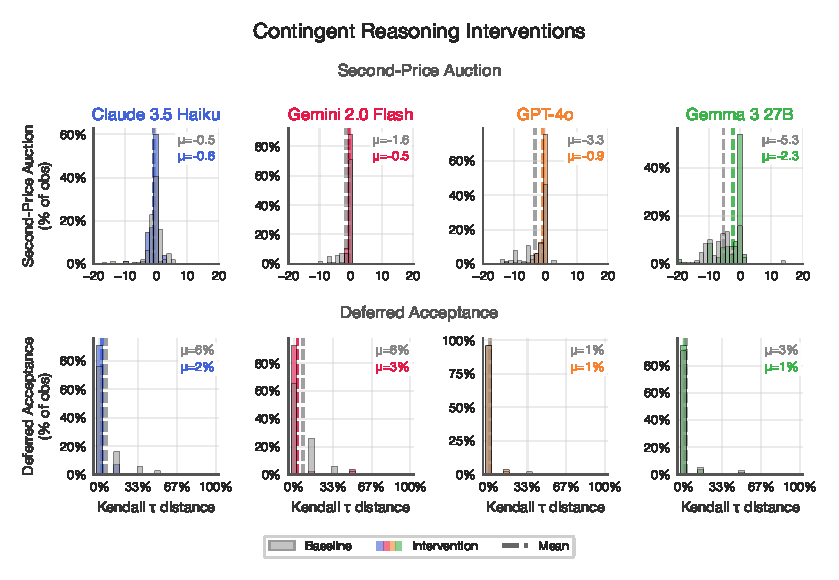
\includegraphics[width=\textwidth]{fig2_contingent.pdf}
    \caption{Contingent reasoning: \emph{Payoff Tree} intervention (C1).
    Second-price auction bid deviations
    ($\text{bid}-\text{value}$) across the four model families; baseline SPSB
    in gray, intervention in color. The payoff-tree scaffold consistently
    improves play across models, roughly halving the distance from truthful.}
    \label{fig:contingent}
\end{figure}

In auctions, \emph{Payoff Tree} reduces the mean deviation from $\mu = -2.67$
to $\mu = -1.13$, roughly halving the distance from truthful play
(Figure~\ref{fig:contingent}). The improvement is consistent across models:
GPT-4o moves from $-3.28$ to $-0.86$, Gemma from $-5.27$ to $-2.34$, and
Gemini from $-1.63$ to $-0.53$; Claude, already close to truthful ($-0.49$),
is the one model showing null improvement. The scaffold closes roughly half
the gap to the OSP benchmark (clock $\mu \approx -0.5$) without changing the
extensive form.

Laying out the payoff tree does not tell models \emph{what} to do; it tells
them \emph{what happens} under each action. This is precisely the cognitive
gap between OSP and non-OSP mechanisms: in OSP mechanisms the extensive form
makes the payoff-relevant contingencies visible at each decision point,
whereas in non-OSP mechanisms the agent must construct them herself. The
\emph{Payoff Tree} scaffold does this construction for the agent, and the
consistent improvement across models suggests that the
difficulty of constructing payoff-relevant contingencies is a real constraint
that binds on LLM agents.

\subsubsection{Belief formation (C3): making opponents salient}
\label{sec:ranking-beliefs}

The third axis is belief formation. \citet{borgers2019strategically}
introduce \emph{strategic simplicity}: a mechanism is strategically simple if
optimal play does not depend on higher-order beliefs about what opponents
believe. Strategy-proof mechanisms are trivially strategically simple---the
dominant strategy is independent of beliefs entirely. Scaffolding belief
formation should therefore be irrelevant at best. But if models are already
treating these mechanisms as Bayesian games, attempting to best-respond to
perceived competition rather than playing the dominant strategy, then making
beliefs more salient could amplify mistakes. We test two levels of belief
scaffolding: \emph{First-Order Beliefs} (``What do you expect
the other players to do? \ldots Does this affect what you should do?'') and
\emph{Second-Order Beliefs} (``What do the other players think YOU will do?
\ldots And does that, in turn, affect what you should do?'').

\begin{figure}[htbp]
    \centering
    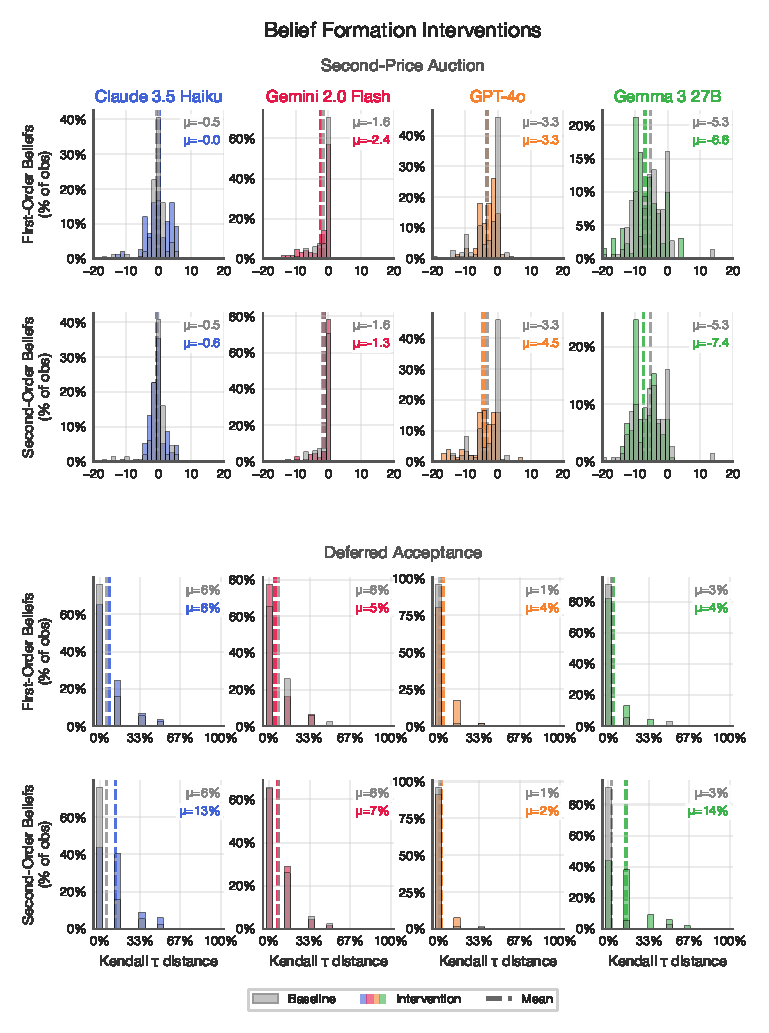
\includegraphics[width=\textwidth,height=0.82\textheight,keepaspectratio]{fig4_beliefs.pdf}
    \caption{Belief-formation interventions (C3): second-price auction bid
    deviations under first-order and second-order belief scaffolds, across the
    four model families. Baseline distributions in gray, interventions in
    color. Belief scaffolds almost uniformly worsen play, with second-order
    beliefs causing the most damage. Gemini is the notable exception, showing
    near-immunity to belief scaffolding.}
    \label{fig:beliefs}
\end{figure}

Belief scaffolding almost uniformly worsens play
(Figure~\ref{fig:beliefs}). In auctions, \emph{First-Order Beliefs} moves the
cross-model mean deviation from $\mu = -2.67$ to $-3.04$ and
\emph{Second-Order Beliefs} to $-3.47$: models prompted to think about
opponents shade further below value, undercutting perceived competition.
Interestingly, Gemini is almost completely immune to belief scaffolding, while
Gemma is the most susceptible to this failure mode. These results suggest that
LLM reasoning styles are not
monolithic; the heterogeneity across model families in susceptibility to
belief-based reasoning may itself be relevant to mechanism design when
markets serve diverse artificial agents.

\subsection{The Ranking Assembled}\label{sec:ranking-synthesis}

Table~\ref{tab:ranking} assembles the preceding cells into the paper's
central object. For each lever we report the raw auction deviations and
the preservation index $\rho$ (Section~\ref{sec:metrics}), computed within
model and pooled as the median across the available cells,
with $95\%$ confidence intervals from a double bootstrap that resamples cells
and propagates each cell's own bootstrap uncertainty (2{,}000 draws, seed
1299). Because $\rho$ is computed against each model's own baseline, the
ranking is invariant to disputes about cross-model levels; it asks only how
much of each model's own deviation a lever removes.

\paragraph{The tier structure, tested.}
Our pre-committed reading of the data is a \emph{tier structure}---a partial
order, not a strict total order:
\begin{equation*}
\underbrace{\text{A}}_{\substack{\text{extensive form:}\\ \text{ascending clock}}}
\;\succ\;
\underbrace{\{\text{B2},\,\text{B3},\,\text{C1}\}}_{\substack{\text{safety descriptions,}\\ \text{clock-framing, payoff tree}}}
\;\succ\;
\underbrace{\text{baseline} \,\approx\, \text{B1}}_{\text{menu restatement}}
\;\succ\;
\underbrace{\text{C3}}_{\substack{\text{belief}\\ \text{scaffolds}}}
\;\succ\;
\underbrace{\text{D-averse.}}_{\substack{\text{risk-averse}\\ \text{persona}}}
\end{equation*}
The concordance statistics now exist, and they support most---not all---of
this structure. Treating each model as a judge ranking the levers, Kendall's
$W$ is $0.70$ in auctions ($p = 0.004$): the lever ordering is far from
independent across models. (This statistic is computed on the corrected
baselines described below; correcting the contaminated axis-2 ``baseline''
cell \emph{raised} auction concordance from $0.43$ to $0.70$---the mislabeled
treatment had been injecting noise into every axis-2 contrast.) Exact
binomial sign tests on adjacent tiers confirm three of the four boundaries:
the extensive form beats the strong presentation tier in $7/8$ cells
($p = 0.070$), the strong presentation tier beats the restatement tier in
$8/8$ ($p = 0.008$), and the strategizing scaffolds beat the risk-averse
persona in $8/8$ ($p = 0.008$).
The boundary that \emph{fails} is baseline-vs-menu against the strategizing
scaffolds: restatements beat lookahead and beliefs in only $4/8$ cells
($p = 1.0$). The failure is informative rather than noise: the menu
restatement is not a clean placebo tier but a sign-mixed family, null on
average (two-sided placebo sign test against baseline: $3/8$ cells above
zero, $p = 0.73$) yet with genuine model-level backfires (GPT-4o's auction
menu cell, Welch $p = 0.003$) that land it below some strategizing cells.

\paragraph{The sharpened story: invariance content is the active ingredient.}
The matching-domain menu cells (new in this draft; Appendix~\ref{app:da})
resolve what the sign-mixed auction menu leaves ambiguous, by splitting the
restatement family in two. A menu description that \emph{includes the
invariance statement}---``your ranking cannot change your obtainable set,
only which school you get within it''---behaves like a safety-exposing
description: pooled error falls from $4.2\%$ to $1.8\%$, with significant
improvements for the two weak-baseline models (Claude $5.8\%$ to $2.1\%$,
Mann--Whitney $p = 10^{-4}$; Gemini $7.6\%$ to $0.3\%$, $p < 10^{-4}$) and
nulls for the strong ones. A menu description that restates the
\emph{computation} without the invariance statement \emph{worsens} play
(pooled $4.2\%$ to $6.9\%$; GPT-4o $1.0\%$ to $4.2\%$, Gemma $2.6\%$ to
$13.7\%$). Together with the auction results, the pattern across all of
family~B is consistent: safety-exposing text (B2, pooled $\rho = +0.90$) and
the invariance-carrying menu variant ($+0.65$) help; mechanical restatement
(auction menu $-0.22$, mechanics-only DA menu $-1.67$) is null-to-harmful.
The active ingredient of an effective description is not restating the
mechanism but asserting the invariant that makes truth-telling safe. The
human experimental record, read through the same split, independently
supports it: invariance-carrying descriptions improve human understanding
and (modestly) behavior in matching mechanisms
\citep{gonczarowski2024describing,katuscak2024simpler}, while
mechanics-only descriptions of a strategy-proof mechanism have been found
to \emph{reduce} truth-telling in the field \citep{guillen2018effectiveness}
---the same backfire our mechanics-only cell produces.

\paragraph{Within-tier order and an honest caveat.}
We deliberately do not order the safety description and the payoff tree within
the strong tier: their pooled preservation indices ($\rho = +0.78$ and
$+0.59$) have overlapping confidence intervals, and the payoff tree beats the
safety description in only $3/4$ of the auction cells, so the data do not
support a strict order between them. Clock-framing, now estimated on
all four models, is a reliable but modest member of the tier
($\rho = +0.29$ $[+0.17, +0.45]$). One caveat from the concordance
analysis qualifies individual cells without moving any rung: what
previously appeared as an anomalously good Gemma axis-2 baseline (SMAD
$8.6\%$ vs.\ $20.7\%$ pooled across its axes) turns out to have a mechanical
explanation: a provenance audit of the run templates shows the legacy
``axis-2 baseline'' cell was not a plain SPSB description at all but a
two-stage sealed-bid-as-clock-exit description---a clock-framing variant
that Gemma responds to strongly (Section~\ref{sec:ranking-descriptions}).
The pooled axis baseline used throughout therefore excludes that cell
(axis-1 and axis-3 cells only), the axis-2 treatment contrasts are computed
against the corrected pool, and the cell itself enters the description
family as a treatment.
\paragraph{The frontier: the ranking compresses, and the failures change kind.}
The full lever grid now also exists for four frontier models (gpt-5-mini,
gpt-5, Claude Sonnet 5, Gemini 2.5 Flash; Appendix~\ref{app:ablations}), and
it turns the frontier scope condition from an extrapolation into a
measurement. Three facts summarize it. First, \emph{the ranking's positive
rungs have nothing left to do}: all four models bid essentially exactly
truthfully at every sealed-bid baseline (mean deviations $0.00$--$0.30$,
SMAD $0$--$2.3\%$), so the safety descriptions, payoff tree, and belief
scaffolds leave play unchanged---the preservation index is undefined as
$D(\text{baseline}) \to 0$, exactly the compression anticipated in
Section~\ref{sec:discussion}. Second, \emph{the backfire rungs retain their
teeth, heterogeneously}: the menu restatement---inert to slightly harmful in
the incumbent grid---collapses Claude Sonnet 5 from exact truthfulness to a
mean deviation of $-\$8.71$ (SMAD $35.5\%$, Cohen's $d = -3.8$,
$p < 0.001$) and degrades Gemini 2.5 Flash (SMAD $2.3\% \to 9.1\%$,
$p < 0.001$), while leaving gpt-5 and gpt-5-mini exactly truthful. The
traces say exactly what broke: under the menu wording, Claude Sonnet 5
announces that ``the standard first-price auction equilibrium bid is
$(n-1)/n$ of my value'' and executes that formula flawlessly---its
$-\$8.71$ is almost exactly the $-\tfrac{1}{3}\,\mathbb{E}[v] \approx
-\$8.17$ the first-price rule implies---despite the prompt stating that
the winner pays the highest \emph{rival} bid. The unfamiliar wording did
not degrade its play into noise; it re-classified the game and retrieved
the wrong textbook solution, executed perfectly. A description with no
incentive content can still break an otherwise perfect strategic reasoner,
and which reasoner it breaks is not predictable from baseline capability. Third, what first appears as an
\emph{inversion of the top rung}---the ascending clock, which improves
every incumbent model, makes Claude Sonnet 5 \emph{worse} than its own
sealed baseline (SMAD $0.27\%$ sealed vs.\ $8.6\%$ clock, $p<0.001$, with
$75\%$ of its exits more than a dollar early)---turns out on inspection to
be the same retrieval failure as the menu cell, not a property of the
extensive form. The clock cells inherit the legacy affiliated-values
\emph{description} (Section~\ref{sec:ranking-extensive}), and Claude
Sonnet 5's exit rationales explicitly invoke the winner's curse (``others'
persistence signals possibly similar high values, risking overpayment''),
a script that is correct in common-value clocks and irrelevant here, where
the bidder knows its own value. Rerunning the same model on the clean
IPV-described clock restores near-perfect play: SMAD $2.0\%$, early exits
$3\%$, and marginal-reasoning traces (``price equals my value; drop'').
One sentence of affiliation language costs an otherwise exactly-truthful
model eight SMAD points by activating the wrong playbook---while the same
sentence leaves the incumbent models' clock gains intact, because they have
no winner's-curse script to misfire. (gpt-5 and gpt-5-mini shift by
$+0.3$--$0.6$ on the clock, mostly tick granularity, with clean marginal
reasoning in their traces.) The design lesson for mixed fleets is asymmetric:
simplifying levers are (at worst) wasted on frontier agents, but
presentation choices can still harm them, so the practitioner guidance of
Section~\ref{sec:discussion}---expose invariants, avoid gratuitous
restatements---remains binding even where the bounded-rationality regime
has closed. (The gpt-5 column carries reduced cell sizes, $K = 5$--$50$:
the model frequently omits the required response tags, and unparseable
repetitions are dropped rather than imputed; Appendix~\ref{app:ablations}
reports per-cell $n$.)

\begin{table}[htbp]
\centering
\footnotesize
\setlength{\tabcolsep}{4pt}
\resizebox{\textwidth}{!}{%
\begin{tabular}{llll cc l l}
\toprule
& & & & \multicolumn{2}{c}{Deviation $D$} & & \\
\cmidrule(lr){5-6}
Tier & Lever & Family & Theory tag & Auct.\ (\$) & DA (\%) & Pooled $\rho$ [95\% CI] & Human anchor \\
\midrule
1 & Extensive form (AC-B clock / iterative DA) & A & OSP \citep{li2017obviously,ashlagi2018stable} & $-0.5$ & 0.0 & $+0.97$ [$+0.83, +1.00$] & AC $+0.62$ [$+0.39,+0.79$]; AC-B $+0.37$ [$-0.12,+0.72$] \\
\midrule
2 & Safety description & B2 & SP-exposing \citep{gonczarowski2023strategyproofness} & $-1.53$ & 0.2 & $+0.78$ [$+0.39, +1.00$] & --- (lab prediction) \\
3$^{*}$ & Menu, invariance property (DA) & B1 & menu + invariant & --- & 1.8 & $+0.65$ [$-0.52, +0.95$] & $\surd$ agrees (sign) \citep{gonczarowski2024describing,katuscak2024simpler} \\
2 & Payoff tree & C1 & contingent reasoning \citep{li2024designing} & $-1.13$ & 1.7 & $+0.59$ [$+0.46, +0.68$] & --- (lab prediction) \\
2 & Clock-framing & B3 & OSP description \citep{breitmoser2022obviousness} & $-1.93^{\dagger}$ & --- & $+0.30$ [$-0.77, +0.52$] & $\surd$ agrees (sign, 3/4 models) \\
\midrule
3 & Baseline (SPSB / direct DA) & --- & --- & $-2.67$ & 4.2 & 0 & $\surd$ agrees \\
4 & Forward planning (lookahead) & C2 & one-step simplicity \citep{pycia2023theory} & $-1.65^{\dagger\S}$ & 7.8 / 5.1 & $-0.00$ [$-2.12, +0.26$] & --- (lab prediction) \\
3 & Menu restatement (auction) & B1 & menu description \citep{gonczarowski2023strategyproofness} & $-2.09^{\dagger}$ & --- & $-0.14$ [$-1.00, +0.27$] & $\surd$ agrees on avg.\ ($-0.07$ [$-0.12,-0.02$]) \\
4 & Second-order beliefs & C3 & strategic simplicity \citep{borgers2019strategically} & $-3.47$ & 9.1 & $-0.35$ [$-1.36, +0.03$] & --- (lab prediction) \\
4 & First-order beliefs & C3 & strategic simplicity \citep{borgers2019strategically} & $-3.04$ & 5.1 & $-0.41$ [$-0.88, -0.04$] & --- (lab prediction) \\
3$^{*}$ & Menu, mechanics only (DA) & B1 & menu, computation restated & --- & 6.9 & $-1.67$ [$-5.01, +0.57$] & $\surd$ agrees (backfire) \citep{guillen2018effectiveness} \\
\midrule
5 & Risk-averse persona & D & preference framing \citep{kahneman1979prospect} & App.~\ref{app:prospect} & App.~\ref{app:prospect} & $-1.82$ [$-5.73, -0.72$] & --- (lab prediction) \\
\bottomrule
\end{tabular}}
\caption{The simplicity-preservation ranking, rows sorted by pooled $\rho$.
$D$ = mean deviation from dominant-strategy play: bid $-$ value in dollars
for auctions (cross-model mean over GPT-4o, Claude 3.5 Haiku, Gemini 2.0
Flash, Gemma 27B), normalized Kendall-$\tau$ error in percent for the
supplementary matching experiment (Appendix~\ref{app:da}; lookahead entries are
one-/two-step). $\rho = 1 - D(\text{lever})/D(\text{baseline})$ on the
absolute-deviation scale, computed within model $\times$ domain against the
baseline conventions of Section~\ref{sec:ranking}; pooled value = median over
available cells, with double-bootstrap $95\%$ CIs (2{,}000 draws, seed 1299).
Tier = pre-committed partial order; within-tier order is not asserted.
$^{*}$New matching-domain menu cells assigned ex ante to the restatement
family (tier 3); their measured positions straddle the ranking---the
invariance-property variant performs like a tier-2 safety description, the
mechanics-only variant like a tier-4 backfire (see text).
$^{\dagger}$Intervention-grid cells tested against pooled-axis baselines
(corrected pool: axis-1 and axis-3 cells only, cross-model mean $-2.55$; see the axis-2 provenance discussion above) rather than the dedicated SPSB cells ($-2.67$).
$^{\S}$The auction C2 cell is a backward-induction \emph{framing} of the
static sealed bid (SPSB has no true planning axis); it enters the pooled
$\rho$ alongside the DA lookahead cells. Human anchor: $\surd$ = a human
experiment exists for this rung and its effect agrees in sign with the LLM
effect (reconstructed human $\rho$ [CI] shown where computable); --- = no
human experiment exists and the rung is issued as a lab prediction
(Section~\ref{sec:humans}).}
\label{tab:ranking}
\end{table}

\begin{figure}[htbp]
    \centering
    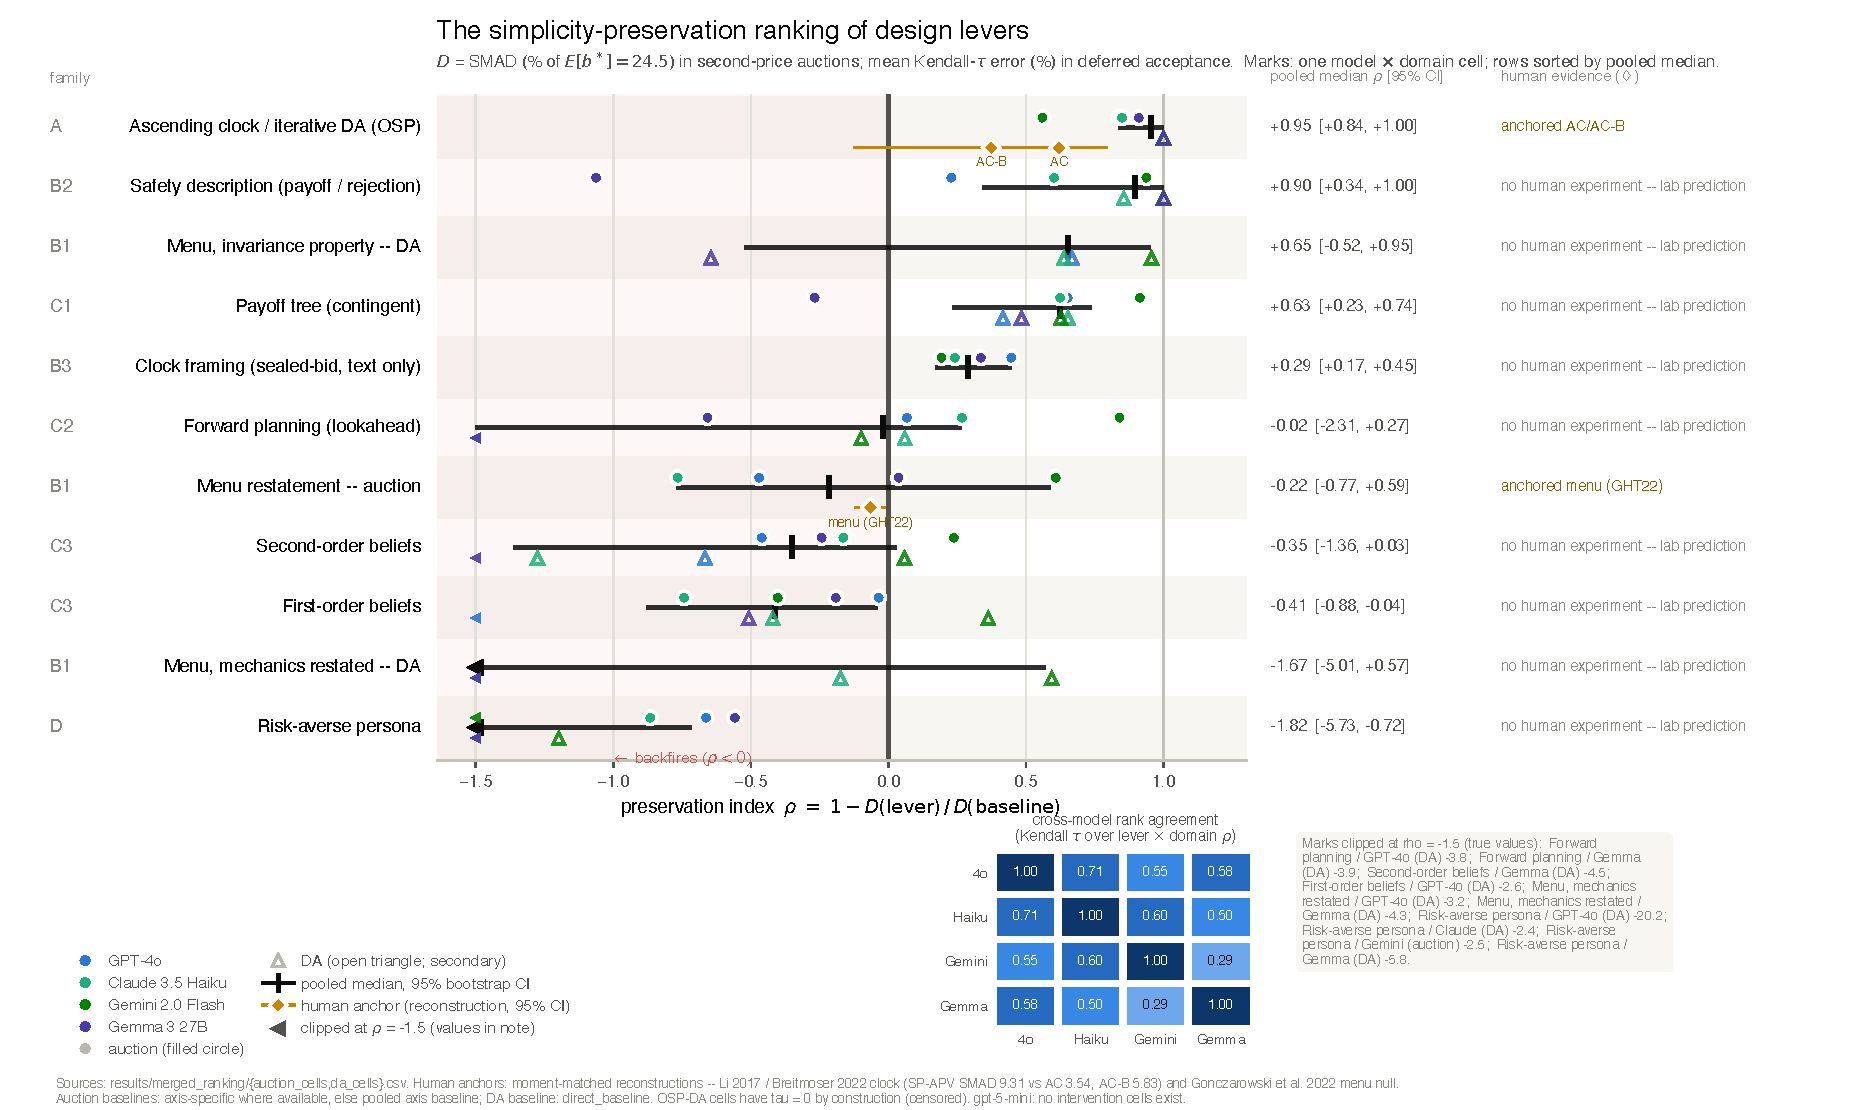
\includegraphics[width=\textwidth]{ranking_forest.pdf}
    \caption{The simplicity-preservation ranking of design levers.
    \emph{Panel A:} rows are levers sorted by pooled median
    $\rho = 1 - D(\text{lever})/D(\text{baseline})$; individual marks show
    each model $\times$ domain cell (color = model, shape = domain), with the
    pooled median and double-bootstrap $95\%$ CI per row; the shaded region
    $\rho < 0$ marks levers that backfire. Gold diamonds are human anchors
    computed from the moment-matched reconstructions
    (Section~\ref{sec:reconstruction}): AC $\rho = +0.62$, AC-B $+0.37$, menu
    $-0.07$; rungs without a diamond have no human experiment and are issued
    as lab predictions (Section~\ref{sec:humans}). Extreme negative
    matching-domain cells are clipped for display (see text). \emph{Panel B
    (inset):} cross-model rank-agreement (Kendall $\tau$) over the lever
    ordering. See Table~\ref{tab:ranking} for the underlying cells.}
    \label{fig:ranking}
\end{figure}

\paragraph{What the ranking localizes.}
Read from the bottom up, the assembled ranking localizes the constraint that
simple mechanism design relieves. Scaffolding strategizing---beliefs,
lookahead---makes play strictly worse, so the problem is not too little
strategic reasoning. Mechanically restating the rules is null on average and
harmful where it displaces the safety-relevant content, so the problem is not
raw comprehension bandwidth either. What works, wherever it appears and in
whatever syntactic form---the safety one-liners, the invariance-carrying menu
variant, the textbook strategy-proofness statement---is text that asserts the
invariant that makes truth-telling safe; and full OSP implementation, which
makes that invariant visible at every decision point, delivers the remainder.
As Section~\ref{sec:ranking-descriptions} put it: the binding cognitive
barrier in non-OSP mechanisms is not \emph{computing} the dominant strategy
given the game tree, but understanding the mechanism well enough to \emph{see
that truth-telling is safe}. The ordering, moreover, parallels the
theoretical hierarchy from which the taxonomy was derived ex ante
(Section~\ref{sec:framework}): the levers that theory says relax binding
cognitive constraints sit at the top, and the levers that theory says should
be irrelevant for strategy-proof mechanisms are, for agents who do not fully
trust that irrelevance, actively harmful. Section~\ref{sec:ranking-traces}
adds a final, mechanism-level piece of evidence: the effective descriptions
move bids \emph{without} changing what the agents say they are doing.
Section~\ref{sec:humans} then closes the loop, anchoring each rung to the
human experimental record where one exists and issuing the unanchored rungs
as predictions.

\subsection{What the Traces Say: Stated Reasoning and Realized Bids}
\label{sec:ranking-traces}

Every bid in our experiments is accompanied by a short free-text plan in
which the agent explains its choice (median 68 words). We analyze all
21{,}990 plans from the sealed-bid and clock cells with a transparent
dictionary of eighteen keyword features---stated intent to shade below or bid above
value, rehearsal of the second-price payment rule, dominance language,
worst-case and profit-margin rhetoric, and explicit mechanism confusion
(calling the auction ``first-price''), among others (full regular expressions
and per-cell prevalence in the replication package,
\path{analysis/build_trace_features.py}).\footnote{The plans are stated
strategies, not full chains of thought; all claims in this subsection concern
what models \emph{say}, with Table~\ref{tab:trace-dissociation} showing that
what they say tracks what they do.}

Two facts establish what the traces are. First, the modal plan applies
\emph{first-price} logic to the second-price auction: $53\%$ of sealed-bid
second-price traces state an intent to bid below value, $55\%$ worry about
``overpaying,'' and $31\%$ invoke a ``profit margin'' or ``buffer,'' while
only $2\%$ use dominance language and only $4\%$ correctly rehearse that the
winner pays the \emph{second}-highest bid; Claude explicitly mislabels the
mechanism ``first-price'' in $10\%$ of its traces, a mistake no other model
makes more than $0.1\%$ of the time. Second, the traces are not cheap talk:
among traces stating an intent to shade, $97.1\%$ of bids fall below value
(mean deviation $-\$1.84$); among traces stating an intent to bid above,
$87.6\%$ fall above ($+\$1.88$); and the largest errors come from the
4{,}541 traces that state no value-anchored intent at all (mean deviation
$-\$4.84$), whose plans anchor on uninformative quantities such as
``slightly above half my value.'' Stated direction almost always matches the
realized bid; the failure is in which plan is chosen. A pooled regression of
$|b - v|$ on the dictionary features nonetheless explains only a modest share
of the error variance (incremental $R^{2} \approx 0.075$ over model and
lever-family fixed effects); the regression table and robustness checks are
in Appendix~\ref{app:traces}.

Most important for interpreting the ranking, the levers of
Sections~\ref{sec:ranking-descriptions}--\ref{sec:ranking-scaffolds} produce
a complete \emph{dissociation} between stated reasoning and behavior
(Table~\ref{tab:trace-dissociation}): across every lever we test, language
and bids never move together. \emph{Payoff Safety} (B2) moves bids
substantially while leaving stated reasoning untouched: the invariant it
asserts (``your bid determines \emph{if} you win, not \emph{what} you pay'')
is echoed in zero of its 600 treated traces, and payment-rule rehearsal is
flat relative to baseline ($2.8\%$ treated vs.\ $3.9\%$, $p = 0.60$); the
plans keep the same shading rhetoric and simply shrink the shade to pennies
(``I will bid \$31.9 to avoid overbidding,'' value \$32). The
\emph{worst-case} scaffold (C1) does the opposite: it massively shifts
stated reasoning (worst-case language rises from $2\%$ to $43\%$) while bids
barely move ($3.24 \to 3.07$, $p = 0.81$). The \emph{Payoff Tree} is a
second bids-only lever: it cuts mean $|b-v|$ from $3.20$ to $1.29$ while
leaving payment-rule rehearsal exactly at its baseline rate ($33.0\%$ vs.\
$32.7\%$, $p = 0.90$)---an earlier reading on which the tree also moved
rule-rehearsal language was an artifact of the contaminated axis-2 baseline
cell documented in Section~\ref{sec:ranking-synthesis}, whose clock
narrative crowded out rule vocabulary. The \emph{menu} restatement moves
neither, serving as the placebo row. Because the first stage is null for
every verbalized-understanding measure, a classical mediation decomposition
bounds the share of Payoff Safety's behavioral effect that could run through
stated comprehension at roughly one third ($95\%$ upper bound $35\%$; point
estimate $\approx 0$), under assumptions the within-treatment association
(rule-rehearsing traces err \$1.5 less, CI $[-2.15,-0.56]$, non-causal)
cannot tighten. Stated comprehension and behavioral improvement are
separable outcomes, and our effective descriptions improve the latter
without the former---which is why we describe them as changing behavior, not
stated understanding, and why the traces should not be read as faithful
mediators of the lever effects.
\TODO{LLM-judge strategy taxonomy (trace option 1): validate the keyword
dictionary against a judged taxonomy on a 100-trace human-labeled set before
the ``2\% dominance recognition'' figure is made load-bearing.}

Finally, the traces speak to \emph{why} comprehension fails. In the GPT-4o
first-price and third-price variants of the same grid, the model deploys a
nearly identical shading script---shading language in $70\%/79\%/72\%$ of
second-/first-/third-price traces and mean bids of $0.88/0.87/0.84$ of
value---even though the optimum differs sharply across formats (truthful in
second-price; roughly $\tfrac{2}{3}v$ in our three-bidder first-price cell;
above value in third-price). The same words justify underbidding where
shading is optimal and where it is an error: the reasoning script is a
property of the model, not of the mechanism it faces.
\TODO{The cross-mechanism script-invariance result is currently
GPT-4o--only (recovered V12 logs); run FPSB/TPSB cells for Claude, Gemini,
and Gemma with the frozen dictionary before claiming generality.}

\begin{table}[htbp]
\centering
\small
\begin{tabular}{lcccc}
\toprule
& \multicolumn{2}{c}{Stated reasoning} & \multicolumn{2}{c}{Behavior} \\
\cmidrule(lr){2-3}\cmidrule(lr){4-5}
Lever (family) & target language & $\Delta$ vs.\ baseline &
mean $|b-v|$ & baseline \\
\midrule
Payoff Safety (B2) & payment-rule rehearsal & $3.9\%\to 2.8\%$ ($p=0.60$) &
$1.95$ ($p=0.015$) & $3.20$ \\
Worst-case scaffold (C1) & worst-case rhetoric & $2\%\to 43\%$ ($p=0.007$) &
$3.07$ ($p=0.81$) & $3.24$ \\
Payoff Tree (C1) & rule rehearsal & $33.0\%\to 32.7\%$ ($p=0.90$) &
$1.29$ ($p=0.017$) & $3.20$ \\
Menu restatement (B1) & --- & --- &
$3.55$ ($p=0.66$) & $3.20$ \\
\bottomrule
\end{tabular}
\caption{Dissociation between stated reasoning and bidding behavior
(pooled over four models, sealed-bid second-price cells; wild-cluster
bootstrap $p$-values clustered at the run level, with model-cluster
permutation cross-checks and duplicate-trace robustness in
\texttt{results/traces/mediation/}). No lever moves both columns: Payoff
Safety and the Payoff Tree improve bids without changing what agents say;
the worst-case scaffold changes what agents say without improving bids; the
menu restatement moves neither. The baseline is the corrected pooled axis
baseline (axis-1 and axis-3 cells only; the legacy axis-2 ``baseline'' cell
was itself a clock-framed description and is analyzed as a treatment in
Section~\ref{sec:ranking-descriptions}); under the dedicated-SPSB convention
the Payoff Safety contrast is the $-2.67 \to -1.53$ of
Section~\ref{sec:ranking-descriptions}. No language entry is reported for the
menu row because the menu prompt replaces the ``second-highest'' vocabulary
wholesale, so rule-rehearsal prevalence is zero by construction (prompt echo,
not comprehension).}
\label{tab:trace-dissociation}
\end{table}

% ============================================================================
% 07_humans.tex — Ordinal Agreement and the Limits of Cardinal Calibration
% (sec:humans). Rewritten in the merge pass: Part 1 = rung-by-rung ordinal
% anchoring (updated to the four-model E3 cells and the canonical direction
% convention); Part 2 = the cardinal-calibration question (tab:cardinal),
% built from results/cardinal/{cardinal_grid.csv,cardinal_summary.md}.
% Human cells are moment-matched reconstructions (sec:reconstruction, app:human).
% ============================================================================

\section{Ordinal Agreement and the Limits of Cardinal Calibration}\label{sec:humans}

The ranking of Section~\ref{sec:ranking} is estimated on populations of LLM agents. This section asks, in two steps, what that ranking is worth to a designer whose participants are human---and, symmetrically, what five decades of human experimental evidence contribute to the credibility of the ranking. The first step is ordinal: on every rung of the ranking where a human benchmark exists, the sign of the treatment effect agrees, even though the two populations make opposite baseline mistakes---a fact we argue converts the validity map's most awkward cell into the strongest available evidence that the ranking measures properties of \emph{mechanisms} rather than of any particular reasoner. The second step is cardinal, and its answer is negative in an instructive way: searching a grid of the tuning knobs available to a practitioner---sampling temperature, risk personas, framing manipulations, rule explanations---we find that no single setting produces cardinal agreement with human play across mechanisms. Level agreement is achievable mechanism by mechanism; direction agreement is achievable with exactly one knob that breaks the level agreement elsewhere; and the best tuning for one model family overshoots badly on another. Together the two steps justify the discipline imposed since Section~\ref{sec:reconstruction}: the testbed is an instrument for signs, orderings, and comparative statics, and the boundary of that instrument is now measured rather than assumed.

\subsection{Rung-by-Rung Ordinal Agreement}\label{sec:humans-rungs}

We walk down the ladder of Table~\ref{tab:ranking}, rung by rung, comparing each lever's effect on LLM play with its effect on human subjects where a human experiment exists. The human-anchored rungs are marked as diamonds in Figure~\ref{fig:ranking}; human quantities below are computed from the moment-matched reconstructions of Section~\ref{sec:reconstruction} and anchored to the original published findings.

\paragraph{Extensive form (Family A).} Clock implementations help humans. \citet{li2017obviously} showed experimentally that ascending clock auctions, which are obviously strategy-proof, produce markedly more dominant-strategy play than the strategically equivalent sealed-bid format, and \citet{breitmoser2022obviousness} replicate and extend this pattern; in our reconstruction, human SMAD falls from $9.31\%$ under the sealed-bid second-price format to $3.54\%$ under AC and $5.83\%$ under AC-B, for a preservation index of $+0.62$ $[+0.39,+0.79]$ (AC) and $+0.37$ $[-0.12,+0.72]$ (AC-B). The same lever helps every model we test, and helps it more: in the harmonized four-model grid, the closed clock cuts SMAD to $1.4$--$5.2\%$ from sealed-bid baselines of $9.5$--$20.7\%$ ($p<0.001$ for all four models; Cohen's $d$ up to $1.00$; Section~\ref{sec:ranking-extensive}). The second Family-A comparison comes from the matching robustness domain (Appendix~\ref{app:da}): the iterative, obviously strategy-proof implementation of DA eliminated every observable misreport for three of the four models,\footnote{The zero is exact for the pick-based query protocol in three of four models (rule-of-three $95\%$ upper bounds of $0.85$--$0.92\%$ on the per-decision error rate); Gemma commits five strict pick errors ($1.6\%$), and an alternative yes/no-question implementation of the same extensive form exposes model-specific failures, most notably Claude's $24.1\%$ rate of false rejections. The rung's zero is a statement about a protocol, not about cognition; Appendix~\ref{app:da} gives the full accounting.} and, to our knowledge, no experiment has tested an OSP implementation of DA with human subjects. That rung is issued as a prediction rather than an anchor, and we return to unanchored rungs below.

\paragraph{Clock-framing (B3).} \citet{breitmoser2022obviousness} show that \emph{describing} the sealed-bid second-price auction as an automatic exit threshold in an ascending clock---changing words, not the mechanism---substantially increases truthful bidding among human subjects. The same one-paragraph description now has four-model support: it reduces SMAD in every family---Claude $9.5\%\to7.2\%$, GPT-4o $11.4\%\to6.3\%$, and Gemma $20.7\%\to13.8\%$ (each $p<0.001$), with Gemini's improvement smaller and not significant ($11.7\%\to9.5\%$, $p=0.097$)---for a pooled preservation index of $+0.29$ $[+0.17,+0.45]$ (Section~\ref{sec:ranking-descriptions}). The sign agrees with the human finding in all four families; the magnitude is uniformly positive but well below the true clock's.

\paragraph{Menu restatement (B1).} In the laboratory experiments of \citet{gonczarowski2023strategyproofness}, a menu description that compresses the dominant-strategy logic of the second-price auction does not meaningfully change human bidding (reconstructed $\rho=-0.07$ $[-0.12,-0.02]$). Across our four model families the restatement has no consistent effect either, but the agreement is an agreement \emph{on average} rather than cell by cell: the effect is null for Gemma ($p=0.94$), moves Claude slightly away from truthful play ($+\$0.88$, $p=0.042$) and GPT-4o more clearly away ($-\$1.32$, $p=0.003$), yet moves Gemini \emph{toward} truthful play ($+\$1.75$, $p<0.001$). Pooling, the effects are small and sign-mixed, and a two-sided sign test cannot reject a zero median ($p=0.73$; Section~\ref{sec:ranking-descriptions})---in sharp contrast to the uniformly signed effects of safety-exposing text. We therefore state this rung's anchor precisely: LLM play is consistent with the human null \emph{on average}, with model-level heterogeneity that the single human point estimate cannot adjudicate. The rung retains its placebo value in one direction---the testbed does not manufacture a reliable gain from restating the mechanics---but it is not the clean, uniformly inert tier the human evidence might suggest.

\paragraph{Baseline.} Both populations deviate under the direct mechanisms. Human subjects systematically overbid in sealed-bid second-price auctions \citep{kagel1993independent, kagel1995individual} and submit dominated rank-order lists in deployed matching mechanisms \citep{rees2018suboptimal}; all four LLM families underbid in SPSB, and all four misreport in the direct-DA robustness domain (Section~\ref{sec:validation}, Section~\ref{sec:ranking}, Appendix~\ref{app:da}).

In sum: the clock helps both populations, the clock-framing description helps both, the menu restatement moves neither on average, and the baseline direct mechanisms fail both. Every rung with a human benchmark agrees in sign, with the menu agreement holding at the pooled level over sign-mixed model cells.

\subsection{Opposite Failures, Common Levers: Substrate Independence}\label{sec:humans-reversal}

The validity map's red cell is the direction reversal: humans overbid in SPSB-IPV---$67.2\%$ of all bids exceed value, and $92.2\%$ of the bids that deviate from value deviate upward---while GPT-4o's deviations are overwhelmingly ($81.6\%$) underbids; the same reversal appears in the APV sealed-bid cell ($64.7\%$ human overbidding against $92.4\%$ GPT-4o underbidding).\footnote{Direction shares depend on the convention. Throughout this section we use the repo-canonical convention---the share of bids strictly above value among \emph{all} bids---under which the human SPSB overbid share is $67.2\%$; conditioning on bids that deviate from value gives $92.2\%$. The directional decomposition of Section~\ref{sec:validation}, which removes a $\pm2\%$ band around the benchmark before classifying, yields slightly different deviator-conditional shares; no conclusion in this paper turns on the choice.} Read as a test of the proxy hypothesis---``LLMs reproduce human behavior''---this cell is a failure, and we declared it as such in Section~\ref{sec:validation}. Read against the ranking, it becomes the paper's sharpest identification result. Two populations fail in \emph{opposite} directions, yet they are corrected by the \emph{same} levers, in the same order: the clock repairs human overbidding and LLM underbidding alike, the clock-framing description does the same, and the menu restatement repairs neither. If the deviations were driven by population-specific psychology---a joy of winning or spite pushing humans above value, a trained conservatism pulling LLMs below it---there would be no reason for a shared correction structure. The parsimonious reading is that the binding constraint lives in the strategic problem itself: in the difficulty of verifying, from a direct mechanism's description, that truth-telling is safe \citep{li2017obviously, oprea2024decisions}. What fills the gap left by that missing verification is population-specific---competitive overbidding in humans, conservative shading in LLMs---but the gap, and the levers that close it, are shared. This is the sense in which the lever ordering is substrate-independent, echoing the hypothesis structure of Section~\ref{sec:framework}.

The reversal also rules out a deflationary explanation of the rung-by-rung agreement. If LLMs merely reproduced human experimental regularities memorized from training corpora, agreement on the levers would be uninformative---but a population imitating the published human data would \emph{overbid} in second-price auctions, and ours does not. The agreement on which levers work is therefore not inherited from the human literature; it is re-derived by a different reasoner failing in a different way.

\paragraph{An out-of-sample prediction.} One tier of the ranking has no human anchor precisely where the ranking is most useful. Safety-exposing descriptions (B2) are the cheapest lever in the designer's toolkit and, on LLM populations, among the most powerful; and the robustness domain sharpens the prediction into a contrast, since there the \emph{same} menu format splits by content---a menu statement that includes the invariance property behaves like a safety description, while a menu that merely restates the outcome computation backfires (Appendix~\ref{app:da}). The closest human evidence is instructive but incomplete: \citet{gonczarowski2024describing} find that a menu-based explanation of DA significantly improved participants' measured \emph{understanding} of strategy-proofness, while average \emph{behavioral} effects were modest. Our decomposition predicts where the behavioral gain is: in descriptions that expose the safety invariant (``your bid determines whether you win, not what you pay''; ``rejections only redirect, never eliminate''), not in descriptions that restate the outcome mapping. Concretely, we predict that in matched human experiments, a Payoff Safety description will shift human SPSB bid distributions toward value where the menu framing of \citet{gonczarowski2023strategyproofness} did not, and that invariance-stating explanations of DA will move behavior where mechanics-restating explanations move only comprehension. The prediction is cheap to test and falsifiable in both directions: the synthetic version of each treatment cell cost roughly \$10 to run, and an incentivized human counterpart is a single-session design at roughly the \$2{,}000 scale of existing description experiments (Table~\ref{tab:cost}).

\subsection{From Ordinal to Cardinal: Is There a Consistent Tuning?}\label{sec:humans-cardinal}

Everything so far is ordinal, and deliberately so: where levels can be compared, they diverge. LLMs \emph{over-comply} in exactly the formats where the levers work best---in the clock implementations, model SMAD of $0.5$--$0.8\%$ sits an order of magnitude below the human $3.5$--$5.8\%$---while in third-price auctions they sit far above any human benchmark. A natural response, and an increasingly common proposal in the literature on LLMs as experimental proxies, is to \emph{tune}: adjust temperature, personas, or framings until the synthetic population matches the human one cardinally, then read levels off the tuned simulator. This subsection asks whether any such tuning exists in our environment, using every knob for which we have data: sampling temperature ($T\in\{0.1,0.5,1.0\}$; GPT-4o, eight mechanisms), risk personas (averse/neutral/seeking; second price for all four models, first and third price for GPT-4o), prospect-theoretic framings (loss/gain/mixed/endowment/WTA--WTP), and rule explanation on/off---a grid of 95 mechanism$\times$knob cells. Distance to the human benchmarks is measured on three axes: \emph{level} (the gap in SMAD), \emph{direction} (the gap in the share of bids above value), and \emph{shape} (Wasserstein-1 distance between the scaled deviation distributions and the moment-matched human reconstructions). Table~\ref{tab:cardinal} reports the core sealed-bid grid.

\begin{table}[t]
\centering
\small
\caption{Cardinal calibration under tuning knobs (GPT-4o, sealed-bid IPV). Each cell reports SMAD\,\% and the share of bids above value; human targets in the top row. SMAD $=100\cdot\mathbb{E}|b-b^{*}(v)|/24.5$ with each environment's own equilibrium $b^{*}$ (FPSB $N{=}3$: $2v/3$; SPSB: $v$; TPSB $N{=}3$: $2v$). $\dagger$: differs from its own baseline at $p<0.05$ (Welch tests for SMAD, two-proportion tests for shares); baselines are the pooled axis baselines (personas), the loss-aversion baseline (frames), and the $T{=}0.5$ anchor (temperature, explanation). The human third-price target is the \citet{kagel1993independent} $n{=}5$ environment, the closest available benchmark for the $N{=}3$ knob cells.}
\label{tab:cardinal}
\begin{tabular}{lcccccc}
\toprule
& \multicolumn{2}{c}{First price} & \multicolumn{2}{c}{Second price} & \multicolumn{2}{c}{Third price ($N{=}3$)} \\
Setting & SMAD & over\,\% & SMAD & over\,\% & SMAD & over\,\% \\
\midrule
\emph{Human target} & \emph{24.8} & \emph{0.4} & \emph{5.6} & \emph{67.2} & \emph{7.7}$^{\,n=5}$ & \emph{89.8} \\
\midrule
Untuned anchor ($T{=}0.5$)   & 28.1 & 0.0  & 8.9  & 16.7 & 108.3 & 19.4 \\
Axis-pooled baseline     & 23.4 & 0.0  & 11.4 & 0.4  & 120.2 & 0.2  \\
Temperature 0.1          & 28.6 & 0.0  & 15.1$^\dagger$ & 10.2$^\dagger$ & 112.5 & 1.3$^\dagger$ \\
Temperature 1.0          & 25.5 & 0.7  & 13.2$^\dagger$ & 9.8$^\dagger$  & 123.7$^\dagger$ & 2.7$^\dagger$ \\
Risk-averse persona      & 15.0$^\dagger$ & 0.0 & 18.3$^\dagger$ & 0.0 & 129.2 & 0.0 \\
Risk-neutral persona     & 20.9 & 0.0 & 11.0 & 2.7$^\dagger$ & 121.3 & 6.7$^\dagger$ \\
Risk-seeking persona     & 28.0$^\dagger$ & 18.0$^\dagger$ & 10.5 & 45.3$^\dagger$ & 105.8$^\dagger$ & 56.5$^\dagger$ \\
WTA--WTP frame           & 23.0 & 0.0  & 7.2$^\dagger$  & 0.0  & 114.0 & 0.0 \\
Rule explanation off     & 28.1 & 0.0  & 8.7  & 16.0 & 111.3 & 12.6$^\dagger$ \\
\bottomrule
\end{tabular}
\end{table}

\paragraph{Level: the best knob is mechanism-specific.} On the level axis alone, cardinal agreement is often achievable---but with a different knob in every format. In FPSB, temperature $1.0$ closes the gap almost exactly (SMAD $25.50$ $[23.49,27.69]$ against a human $24.76$; untuned anchor $28.11$). In SPSB, the WTA--WTP frame is best ($7.24$ $[6.02,8.56]$ against $5.65$; $-3.57$ SMAD relative to its own baseline, Welch $p=0.005$), while both temperature deviations from the anchor make play \emph{worse}. In the affiliated-values sealed-bid format the untuned anchor is already the best available cell ($10.95$ against $9.31$). The clock formats invert the problem: LLMs are \emph{too good}---SMAD $0.83$ (AC) and $0.48$ (AC-B) against human targets of $3.54$ and $5.83$---so the only knob that moves them toward humans is raising temperature to $1.0$, which works purely by injecting noise into near-perfect play.\footnote{The high-temperature closed-clock cell is small ($8$ non-winner exits); we read the clock rows as suggestive. Two grid cells are unavailable (both clock formats at $T{=}0.1$), and the third-price persona and frame cells exist only at $N{=}3$.} And third-price auctions are not tunable at all: the best third-price cell anywhere in the grid has SMAD $44.1$ (temperature $0.1$, $N{=}5$) against a human $7.66$, and at $N{=}3$---where the equilibrium bid is $2v$---every persona and frame cell sits at SMAD $106$--$131$, because the models bid approximately their value under every setting.

\paragraph{Direction: one knob moves it, at a price.} The direction axis is where the human--LLM reversal of Section~\ref{sec:humans-reversal} lives, and exactly one knob addresses it. Under the risk-seeking persona, GPT-4o's share of above-value bids rises from $0.4\%$ to $45.3\%$ in SPSB and from $0.2\%$ to $56.5\%$ in third price (both $p<10^{-4}$), against human targets of $67.2\%$ and $89.8\%$---direction gaps fall from $66.8$ to $21.9$ percentage points and from $89.6$ to $33.3$. The same persona also improves the third-price \emph{level} ($-14.4$ SMAD, $p=0.011$) and the second-price \emph{shape} (Wasserstein-1 from $23.8$ to $14.8$ points). No other knob moves direction: under every temperature, frame, and explanation setting, the SPSB overbid share never exceeds $17\%$, and the risk-averse persona drives all overbid shares to zero. But the price is paid in first price, the one format where humans almost never bid above value: the risk-seeking persona induces dominated bids in $18.0\%$ of FPSB decisions (human: $0.4\%$; $p<10^{-4}$) and raises FPSB SMAD by $4.6$ points ($p=0.002$). In the direction rankings the same setting is first of fifteen in both SPSB and third price and \emph{last} of fifteen in FPSB---the sharpest possible statement of the trade-off. Matching human overbidding where humans overbid requires a disposition that violates the sharpest regularity humans display where they do not.

\paragraph{Tuning is model-specific.} The trade-off does not even transfer across model families. The same risk-seeking persona applied to SPSB moves Gemma from $20.7$ to $5.87$ SMAD---against the human $5.65$, the single best cardinal match in the grid---and Gemini from $11.7$ to $4.9$, but leaves GPT-4o essentially unchanged ($11.4$ to $10.5$) and explodes Claude from $9.5$ to $35.0$, with $93\%$ of bids above value. A persona calibrated on one model family, then deployed on another, can convert mild underbidding into catastrophic overbidding.

\paragraph{The remaining knobs are not dials.} Temperature is non-monotone where it matters: SPSB SMAD is $15.1$, $8.9$, and $13.2$ at $T=0.1$, $0.5$, and $1.0$ respectively (both deviations from the anchor significant at $p\le10^{-4}$), so it cannot be used to trade off fidelity smoothly; its only clean cardinal use is adding human-like noise to the too-perfect clock formats. Turning the rule explanation on or off has no detectable effect on any axis (level differences of at most $0.16$ SMAD in the first-, second-, and affiliated-value formats, all $p\ge0.53$).\footnote{We phrase this as ``no detectable effect'' rather than as an estimated effect of removing explanation: the manipulation cannot be verified from the archived prompts, and the contrast rests on the run directories' provenance.} The remaining prospect-theoretic frames mostly \emph{hurt} the second-price level relative to their own baseline.

\paragraph{Verdict.} There is no single consistent tuning. Formally: no setting in the grid is in the top half of both the level ranking and the direction ranking on all three core mechanisms; the level winner by worst-case rank (the WTA--WTP frame) and the direction winner (the risk-seeking persona) are disjoint, and the direction winner breaks the level axis in first price. Cardinal agreement is therefore achievable only mechanism-by-mechanism, and sometimes only model-by-model---a boundary that is structural rather than an accident of our grid, since the direction axis demands a disposition that the first-price format punishes. Two implications follow. First, the boundary bounds the proxy use-case: a designer who needs calibrated \emph{levels}---revenue predictions, welfare magnitudes---cannot obtain them from a single tuned synthetic population that spans mechanisms, which is why every cross-population claim in this paper is ordinal. Second, it clarifies what \emph{would} be needed: per-mechanism (and, our results add, per-model) calibration against a small sample of human data from the target environment, in the spirit of \citet{corrigan2025usefulness}---a local correction that our grid suggests cannot be amortized across formats, because the knob that fixes one format's distribution is the knob that breaks another's.

% ============================================================================
% 08_discussion.tex — Discussion (sec:discussion)
% Per plan/plan.md §3 row 8: design implications + practitioner box (Design-C
% graft) + scope conditions + one reconciled cost table (tab:cost, mined from
% writeup/contents/limitation.tex — that file IS the old Discussion) +
% limitations. Merge pass: scope conditions rewritten to the genuine
% gpt-5-mini cells (constraints migrate, not vanish); traces double-
% dissociation paragraph added; practitioner box and limitations updated to
% the invariance-content story and the rescoped DA observability accounting.
% ============================================================================

\section{Discussion}\label{sec:discussion}

\subsection{Design Implications}\label{sec:discussion-implications}

The ranking's most actionable feature is that a nearly costless lever sits close to its top. A one- or two-sentence honest description of a mechanism's safety invariant recovers a large share of what a full obviously strategy-proof redesign buys, without touching the allocation rule, the message space, or the extensive form: Payoff Safety cut the cross-model auction deviation from $-\$2.67$ to $-\$1.53$, and the clock-framing description substantially reduced SMAD in three of the four model families while backfiring in the fourth (pooled $\rho=+0.30$, wide interval; Section~\ref{sec:ranking-descriptions}). The supplementary matching experiment pushes the same point further: Rejection Safety cut direct-DA error from $4.2\%$ to $0.2\%$, and a plain textbook statement of strategy-proofness drove it to $0.0\%$ in all four models (Appendix~\ref{app:da}). For a platform whose participants increasingly include LLM agents, these are deployable as interface text or API documentation at approximately zero engineering cost. They are also honest in the sense of \citet{gonczarowski2023strategyproofness}: they state true properties of the mechanism rather than steering behavior through misdirection, so a designer can adopt them without incurring the credibility costs of manipulative framing. The comparison with restatements disciplines the recommendation, and more sharply than a simple placebo: it is not ``more explanation'' that helps. Menu restatements of the auction are null on average and sign-mixed across models (Section~\ref{sec:ranking-descriptions}), and in the matching domain the same menu format splits by content---a menu that includes the invariance statement improves play like a safety description, while a menu that merely restates the outcome computation makes play significantly \emph{worse} (Appendix~\ref{app:da}). The active ingredient is the invariance content, not the explanation.

As LLMs increasingly participate in markets, the design of the mechanisms they interact with will matter. Our results suggest that simple mechanisms, and clear (and honest) descriptions of mechanism properties, can serve as a form of alignment: channeling artificial agents toward the outcomes the mechanism was designed to produce, without requiring that they fully understand why. And because every lever with a human anchor moves human participants in the same direction it moves LLM agents (Section~\ref{sec:humans}), a designer serving a mixed human--AI market need not choose between populations: simplicity, on this evidence, is a common good across participant types.

The reasoning traces add a caution about \emph{how} these text levers work---and about how their efficacy should be audited. The dissociation of Section~\ref{sec:ranking-traces} shows that the effective levers change behavior without changing stated reasoning: Payoff Safety cuts the mean absolute deviation from $\$3.20$ to $\$1.95$ while its invariant is echoed in none of the six hundred treated traces and the rate of correct payment-rule statements is flat, so a classical mediation analysis fails at the first stage and bounds any comprehension-mediated share of the effect at roughly one third; the payoff tree behaves the same way (bids move, rule-rehearsal language does not). Conversely, the worst-case scaffold visibly changes what models say---worst-case language jumps from $2\%$ to $43\%$ of traces---without moving bids, and the menu restatement moves neither: across every lever tested, language and bids never move together. The channel through which descriptions operate is therefore behavioral rather than deliberative: the text changes what agents \emph{do} without passing through what they \emph{articulate}. For practitioners this cuts in both directions. A designer cannot certify a description by checking that agents verbalize the right principle (the best lever produces no such verbalization), and cannot dismiss one because comprehension checks fail; symmetrically, a passed manipulation check on stated reasoning is no evidence that behavior has moved. Interventions on LLM participants should be evaluated on realized play, not on elicited understanding.

The backfiring tier carries an equally practical warning. Forward-planning and belief-formation scaffolds are not exotic: they are precisely the kind of ``think ahead, model the other side'' instructions that agent frameworks and prompt libraries routinely inject into deployed LLM pipelines \citep{fish2024algorithmic}. In strategy-proof environments, our evidence says such instructions are at best inert and at worst substantial liabilities, with the damage concentrated in the weakest models (Section~\ref{sec:ranking-scaffolds}). We summarize the operational content of the ranking as follows.

\begin{center}
\fbox{\begin{minipage}{0.93\linewidth}
\vspace{0.4em}
\textbf{Practitioner guidance: fielding strategy-proof mechanisms to LLM participants.}
\begin{itemize}[leftmargin=1.4em, itemsep=2pt, topsep=3pt]
    \item \emph{Prefer OSP implementations where available.} The ascending-clock format produced the best play in every model we measured, consistent with its record in human markets \citep{li2017obviously, milgrom2020clock}.
    \item \emph{If you must keep a direct mechanism, state its safety invariant---do not merely restate its mechanics.} Add a safety-exposing sentence (``your bid determines \emph{whether} you win, not \emph{what} you pay''; ``rejections only redirect, never eliminate'') and, where the interface permits, a payoff-tree explanation of what happens under each outcome. Each is a one-paragraph text change; each independently closed roughly half the gap to the OSP benchmark in auctions, and the safety description nearly closed it in DA. Mechanical restatements of the outcome mapping are useless-to-harmful: menu-style restatements were null on average and sign-mixed in auctions, and a menu that restated the computation \emph{without} the invariance statement significantly worsened matching play. The invariance content is the active ingredient.
    \item \emph{Never prompt agents to plan ahead or to model opponents.} Lookahead and belief-formation scaffolds worsened play in nearly every configuration tested---most severely for the weakest models---by activating strategizing that the mechanism makes unnecessary.
    \item \emph{Audit vendor ``reasoning enhancements'' as potential backfire levers.} Agent frameworks that silently inject planning steps or opponent modeling into prompts are, in our taxonomy, Family-C interventions of the backfiring kind; benchmark them against truthful play before deployment.
\end{itemize}
\vspace{0.2em}
\end{minipage}}
\end{center}

\subsection{Scope Conditions}\label{sec:discussion-scope}

The ranking is a statement about a bounded-rationality regime, and both of its boundaries are measured rather than assumed. The upper boundary is now measured with the full lever grid rather than inferred from baseline play alone: we ran the complete intervention battery on four frontier reasoning models (gpt-5-mini, gpt-5, Claude Sonnet 5, Gemini 2.5 Flash; Section~\ref{sec:ranking-synthesis}, Table~\ref{tab:frontier-grid}), and the picture is three-sided. First, the ranking's positive rungs \emph{compress to nothing}: all four models bid essentially exactly truthfully at every sealed-bid baseline (mean deviations $0.00$--$0.30$, SMAD $0$--$2.3\%$), so safety descriptions, the payoff tree, and belief scaffolds leave play unchanged---the preservation index $\rho$ of Section~\ref{sec:metrics}, a ratio to the baseline deviation, becomes uninformative as $D(\text{baseline}) \to 0$. Second, the constraints \emph{migrate} rather than vanish across formats: gpt-5-mini plays second price and (correctly shaded) first price essentially perfectly, yet still fails the harder third-price format outright, bidding roughly its value where the equilibrium calls for bidding above it (three-bidder mean deviation $+\$14.76$; SMAD $60\%$; Appendix~\ref{app:ablations}), so wherever equilibrium reasoning is genuinely required a bounded-rationality regime persists even at the frontier. Third, and the reason compression is not the whole story, \emph{the backfire rungs keep their teeth}: the menu restatement collapses Claude Sonnet 5 from exact truthfulness to a $35.5\%$ deviation ($d=-3.8$, $p<0.001$) and degrades Gemini 2.5 Flash, and one sentence of affiliation language in a clock description triggers a misapplied winner's-curse script in the same model (SMAD $0.3\% \to 8.6\%$), removed entirely by an IPV-worded rerun (Section~\ref{sec:ranking-synthesis}). The frontier failure mode is thus \emph{retrieval selection}: surface wording chooses which memorized playbook runs, and a wrong match is executed flawlessly. A presentation choice with no incentive content can still break an otherwise perfect strategic reasoner, so the practitioner guidance above remains binding even where the simplifying levers have nothing left to preserve. Our main model grid deliberately comprises well-established, widely deployed model families rather than frontier reasoning models: the design question requires agents capable enough to parse the rules of a mechanism yet still susceptible to the reasoning failures that simple design aims to remedy. Deployed fleets will occupy this regime for the foreseeable future: high-volume agentic transactions run on small, cheap models for cost and latency reasons, so the population of economic agents that mechanisms will actually face looks more like our grid than like the frontier. At the lower boundary, Llama-3-8B posts a mean SMAD of $57.58\%$---worse than the reconstructed human benchmark in six of seven formats (Appendix~\ref{app:ablations})---indicating a capability floor below which agents cannot reliably parse the mechanism at all, and beneath which no descriptive lever can be expected to help. The ranking applies to the wide band between these boundaries.

\subsection{What the Testbed Costs}\label{sec:discussion-cost}

The traditional instruments for questions like ours are incentivized human experiments and observational field data, and both are expensive ways to search a large design space: the laboratory test of obvious strategy-proofness engaged 548 subjects across a main experiment and a one-shot follow-up, with documented payments on the order of \$5{,}400 for the main experiment alone \citep{li2017obviously}; incentivized description experiments recruited 542 subjects with average payments of \$15--26 per subject \citep{gonczarowski2024describing}; and observational platform data require controls for seller and bidder heterogeneity that complicate the causal inference a lever ranking needs \citep{manning2024automated}. The synthetic testbed sits at the exploratory end of this pipeline, extending the cost reduction that online laboratories brought to behavioral economics \citep{horton2011online}: the full battery reported in this paper---more than 1{,}000 auctions and 5{,}000 individual agent decisions across two domains, four model families, and the complete lever grid---cost under \$400 in API fees, and a single treatment cell of 50 repetitions costs roughly \$10 (Table~\ref{tab:cost}). These economics are most useful read jointly with Section~\ref{sec:humans}: cheap synthetic screening ranks the candidate levers; expensive human experiments are reserved for the rungs where the ranking makes novel, falsifiable predictions.

\begin{table}[t]
\centering
\small
\resizebox{\textwidth}{!}{%
\begin{tabular}{@{}llll@{}}
\toprule
\textbf{Instrument} & \textbf{Population} & \textbf{Scale} & \textbf{Approx.\ cost} \\
\midrule
OSP laboratory experiment \citep{li2017obviously} & Human & 548 subjects (144 main $+$ 404 follow-up) & $\approx\$5{,}400^{\dagger}$ \\
Description experiments \citep{gonczarowski2024describing} & Human & 542 subjects, incentivized lab & \$15--26/subject$^{\ddagger}$ \\
This paper: full lever battery & LLM ($4$ families) & $>$1{,}000 auctions; $>$5{,}000 decisions & $<\$400$ \\
This paper: one treatment cell & LLM & $50$ repetitions & $\sim\$10$ \\
\bottomrule
\end{tabular}}
\caption{Approximate cost of instruments for testing simplicity-preserving design levers. $^{\dagger}$\citet{li2017obviously}'s main experiment paid 144 subjects an average of \$37.54 (including a \$20 show-up fee), $\approx\$5{,}400$ total; documented for the main experiment only. The paper's one-shot follow-up added 404 subjects (\$5 show-up plus incentive payments), for 548 subjects overall, but does not report an average payment for the follow-up, so a total cost across both experiments is not recoverable from the published figures. $^{\ddagger}$\citet{gonczarowski2024describing} paid Prolific participants an average of £15.0 ($\approx\$19$) and Cornell participants an average of \$25.5 across $542$ subjects (Appendix A.1 of that paper).}
\label{tab:cost}
\end{table}

\subsection{Limitations}\label{sec:discussion-limitations}

\paragraph{The human reconstruction is model-based.} Our human benchmarks are moment-matched mixture reconstructions of published summary statistics, not raw experimental microdata (Section~\ref{sec:reconstruction}, Appendix~\ref{app:human}). We therefore confine human--LLM comparisons to rankings, directions, and comparative statics, attach no significance tests to reconstructed levels, and note that the ranking itself (Section~\ref{sec:ranking}) never conditions on the reconstructions---they anchor transferability only. \TODO{Reconstruction-uncertainty bootstrap bands on every human anchor (Appendix~\ref{app:human}) pending.}

\paragraph{Prompt-template specificity.} Each lever is instantiated as one template per domain, so the estimated effects are, strictly, effects of particular wordings. Three features argue against a prompt-engineering artifact: the taxonomy was fixed ex ante from published theory (Section~\ref{sec:framework}), the menu restatement functions as a built-in restatement control (null on average, though sign-mixed across models; Section~\ref{sec:ranking-descriptions}), and half the taxonomy backfires---a pattern opportunistic prompt search would not produce and would not publish. But invariance to paraphrase remains an assumption rather than a measurement. \TODO{Paraphrase robustness: three paraphrases $\times$ two headline levers (plan \S6).}

\paragraph{Direction shares are convention-dependent.} Statements about the \emph{direction} of deviations (overbidding versus underbidding shares) depend on the classification convention---whether shares are taken over all bids or only over bids that deviate from value, and how a tolerance band around the benchmark is drawn. We use the repo-canonical convention throughout Section~\ref{sec:humans} (share of bids strictly above value among all bids; the human SPSB overbid share is $67.2\%$, or $92.2\%$ among deviating bids), while the directional decomposition of Section~\ref{sec:validation} removes a $\pm2\%$ band before classifying. The qualitative reversal---humans overbid, LLMs underbid---is robust to the choice, but individual shares should not be compared across conventions.

\paragraph{Model-version dependence.} All results are estimated on pinned model snapshots (Section~\ref{sec:design}); provider updates, changes to default system prompts, and fleet turnover can shift behavior in ways we cannot forecast. The ranking should be read as a measurement protocol to be re-estimated as agent populations evolve, not as a constant of nature---and the frontier migration documented above, with dominant-strategy formats solved first and equilibrium-reasoning formats persisting, already indicates the likely direction of drift.

% ============================================================================
% 09_conclusion.tex — Conclusion (sec:conclusion), ≤0.5pp per plan §3.
% Merge pass: auctions main + matching-as-robustness phrasing; sharpened
% invariance-content claim; cardinal verdict as an honest boundary; frontier
% migration (not compression) per the genuine gpt-5-mini cells.
% Cut per plan §7: no nation-scale voting, no risk-aversion claim,
% no combinatorial-auction futures.
% ============================================================================

\section{Conclusion}\label{sec:conclusion}

Which levers available to a mechanism designer keep dominant-strategy play intact for boundedly rational agents? Across sealed-bid auctions---the paper's main domain---and four LLM families, with the pattern reproduced in a school-choice matching domain as a robustness check (Appendix~\ref{app:da}), the answer is a stable hierarchy of tiers. Obviously strategy-proof extensive forms sit at the top. A strong second tier contains levers that change no rule of the game, and its content is sharper than ``more explanation helps'': the active ingredient is the \emph{invariance}. Honest text that exposes why truth-telling is safe, and scaffolds that lay out the mechanism's payoff contingencies, deliver large gains---while restatements of the mechanics carry none of it, coming in null on average and sign-mixed in auctions and actively harmful in matching when the invariance statement is omitted. Below the baseline, scaffolds that prompt agents to plan ahead or to model opponents actively backfire, most severely for the weakest models. The ordering parallels the theoretical simplicity hierarchy built for human reasoners, and it localizes the binding constraint: not \emph{computing} the dominant strategy, but \emph{seeing} that truth-telling is safe.

The human experimental record agrees in sign on every rung where it speaks, at the pooled level---clock formats, clock-framing (in three of four families), the menu restatement's null, invariance-carrying versus mechanics-only descriptions, the failing baselines---even though the two populations fail in opposite directions, which is precisely why the agreement is informative: the constraints, and the levers that relieve them, belong to the strategic problem rather than to any one kind of mind. The agreement is ordinal, and we measure that boundary rather than assume it: no single tuning of the agents---temperature, risk personas, framings, explanations---produces cardinal agreement with human play across mechanisms, because level calibration is mechanism- and model-specific and the one knob that restores the human direction of error in second- and third-price auctions breaks first-price play. The testbed ranks levers; it does not simulate levels. Where the human record is silent, the ranking speaks first: its sharpest untested claim is that safety-exposing descriptions will deliver for human subjects the behavioral gains that mechanical restatements have not---a prediction testable in a single incentivized session at a small fraction of the cost of the synthetic program that generated it.

Three directions strike us as most valuable. First, frontier tracking: the constraints migrate rather than vanish as capability grows---the four frontier models we test master the dominant-strategy sealed-bid auction, yet a content-free menu restatement still collapses one of them, and the third-price format still defeats the frontier where we can measure it---so the ranking should be re-estimated on the formats and presentation margins where reasoning still binds as deployed fleets evolve. Second, combining complementary levers---pairing a safety-exposing description with a payoff-tree scaffold---to trace the minimal intervention that closes the gap to the rational benchmark. Third, the method itself: cognitive scaffolds as diagnostic probes, together with the heterogeneity we document across model families, offer a general way to characterize the structure of an artificial agent's reasoning failures---in mechanism design and beyond.


\ifanon
\paragraph{Disclosure.} An AI assistant was used to assist with plotting code, manuscript restructuring, and consistency review; details withheld for anonymous review.
\else
\paragraph{Disclosure.} Claude (Anthropic) was used to assist with plotting code, manuscript restructuring, and consistency review.
\fi

\bibliographystyle{plainnat}
\bibliography{auction_v2}

\newpage
\appendix
% ---------------------------------------------------------------------------
% Appendix: Human Data Reconstruction
% Source: writeup/contents/appendix.tex:1-98 (reuse, citation + terminology fixes)
% NEW: closing paragraph on reconstruction uncertainty (plan §3 row A, Design C graft)
% ---------------------------------------------------------------------------
\section{Human Data Reconstruction}\label{app:human}

This appendix records, source by source, how we map the aggregate statistics reported in each human experiment into the unified SMAD metric of Section~\ref{sec:metrics}. The mixture model used to reconstruct bid-level distributions is specified in Section~\ref{sec:reconstruction}; the calibrated parameters for every source--treatment pair appear in Appendix~\ref{app:mixture} below, and the closing paragraph of this appendix states exactly which forms of uncertainty our reconstruction bands do and do not capture.

\paragraph{Li (2017) and Breitmoser--Schweighofer-Kodritsch (2022): SPSB, AC, and AC-B under APV.}
These papers \citep{li2017obviously,breitmoser2022obviousness} report mean absolute deviation (MAD)\footnote{For clock auctions, since the winner did not submit a final sealed bid, the reported MAD is computed only from bidders who revealed a bid by dropping out (i.e., those who exited the clock), excluding the winner's unobserved terminal willingness-to-pay.}
from truthful bidding. In \citet{li2017obviously}, the reported deviation is based on a group-level statistic involving the second-highest bid and second-highest value; in \citet{breitmoser2022obviousness}, deviations are computed from submitted bids (often focusing on non-winning bids). In each case we adhere to the source paper's unit of observation, but the SMAD definition conceptually applies to the underlying submitted bids.
Because the equilibrium optimum under AC and SPSB is truthful bidding $b^\star(v)=v$, we have $d_m=|b-v|$ and thus
\[
\Delta_m = 100\cdot \frac{\mathrm{MAD}_m}{\mu_m^\star},
\qquad
\mu_m^\star=\mathbb E[v].
\]
Here $\mathbb E[v]$ is implied by the experimental value distribution reported by the source paper: $\mathbb E[v]=70$ in \citet{li2017obviously}, and $\mathbb E[v]=65$ in \citet{breitmoser2022obviousness} given their stated common-value and idiosyncratic components.\footnote{When auctions are repeated, we follow the source paper's convention and report post-learning blocks (e.g., dropping the first three rounds and using the next reported block).}
If the paper reports $\mathrm{SE}(\mathrm{MAD}_m)$ (often using group means as the unit of observation), we propagate it via
\[
\mathrm{SE}(\widehat{\Delta}_m)=100\cdot \frac{\mathrm{SE}(\widehat{\mathrm{MAD}}_m)}{\widehat{\mu}_m^\star},
\quad
\mathrm{CI}_{95\%}(\Delta_m)=\widehat{\Delta}_m \pm 1.96\,\mathrm{SE}(\widehat{\Delta}_m).
\]

\paragraph{Kagel and Levin (1993): FPSB, SPSB, and TPSB under IPV.}
\citet{kagel1993independent} report bid regressions and over-/under-bidding frequencies for fixed bidder counts (e.g., $N\in\{5,10\}$). We treat each $N$ separately: the regression form $\hat b(x)=\hat\alpha+\hat\beta x$ is fit for a \emph{fixed} number of bidders, and is not pooled across varying $N$.
Theory gives linear equilibrium bid functions under IPV with $x\sim U[x_{\min},x_{\max}]$:

$$\begin{aligned}
b^\star_{\mathrm{FPSB\text{-}IPV}}(x) &= x - \frac{x-x_{\min}}{N} = \frac{N-1}{N}x + \frac{1}{N}x_{\min} \\
b^\star_{\mathrm{SPSB\text{-}IPV}}(x) &= x \\
b^\star_{\mathrm{TPSB\text{-}IPV}}(x) &= x + \frac{x-x_{\min}}{N-2} = \frac{N-1}{N-2}x - \frac{1}{N-2}x_{\min}
\end{aligned}$$

(When $x_{\min}=0$, these reduce to the familiar slope-only formulas.)
Because only summary moments are reported, we reconstruct the bid distribution via a parametric data-generating process (DGP) consistent with the bid regressions and over-/under-bidding frequencies reported in Table~2 of \citet{kagel1993independent}.
For each auction series and fixed $N$, we assume $x\sim U[x_{\min},x_{\max}]$ (bounds from the source paper), and generate bids as
\[
b = \hat\alpha+\hat\beta x + \varepsilon,\qquad \varepsilon\sim \mathcal N(\mu,\sigma^2),
\]
where $(\mu,\sigma)$ are calibrated by moment matching to the reported frequencies (e.g., $\Pr(b>x)$ and $\Pr(b>b^\star(x))$).
Given the calibrated DGP, we estimate
\[
\widehat{\mathrm{MAD}}_m = \mathbb E\!\left[\,|b-b^\star(x)|\,\right],
\qquad
\widehat{\mu}_m^\star=\mathbb E[b^\star(x)],
\qquad
\widehat{\Delta}_m = 100\cdot \frac{\widehat{\mathrm{MAD}}_m}{\widehat{\mu}_m^\star}.
\]
In practice, we run the Monte Carlo procedure 100 times and report the across-run mean $\widehat{\Delta}_m$ as the point estimate; uncertainty is obtained from across-run variability (percentile or normal approximation).

\paragraph{Levin, Kagel, and Richard (1996) and related CV papers: first-price CV and English (second-price proxy).}
In common-value auctions \citep{levin1996revenue}, bidders observe signals $s_i$ about a common value $V$ (e.g., $s_i=V+\varepsilon_i$ as specified in the original paper).

Theory gives the following equilibrium bid functions under common values:
$$\begin{aligned}
b^\star_{\mathrm{FPSB\text{-}CV}}(x) &= x - \epsilon + Y\\
Y &= \left( \frac{2\epsilon}{N+1} \right) \exp\left[ -\left( \frac{N}{2\epsilon} \right) (x - (\underline{x} + \epsilon)) \right]\\
b^\star_{\mathrm{SPSB\text{-}CV}}(x) &= x
\end{aligned}$$

The theoretical benchmark is the equilibrium bidding strategy $b_m^\star(s)$ implied by the source paper's signal structure and mechanism. We therefore compute SMAD \emph{on bids} exactly as in private values:
\[
d_m = |b - b_m^\star(s)|,
\qquad
\Delta_m = 100\cdot \frac{\mathbb E[|b-b_m^\star(s)|]}{\widehat{\mu}_m^\star}.
\]

Because there is a very large common part in each player's valuation, we take the following normalization factor:
\[
{\widehat{\mu}_m^\star} = \mathbb E[b^\star_{max}(x) - b^\star_{min}(x)]
\]

When micro-data are unavailable, we reconstruct the bid distribution by simulating the source paper's DGP (signals and value draws) together with the theoretical bidding rule $b_m^\star(\cdot)$, and calibrate any auxiliary noise parameters by moment matching to the summary statistics reported (e.g., frequencies of overbidding/high bids, or mean prices/profits as available). We run Monte Carlo 100 times and report the across-run mean $\widehat{\Delta}_m$ as the point estimate; uncertainty is obtained from across-run variability (percentile or normal approximation).

\subsection{Mixture-Model Calibration Details}\label{app:mixture}

Table~\ref{tab:mixture-calibration} reports the calibrated parameters of the three-component mixture model of Section~\ref{sec:reconstruction} for every source--treatment pair. The mixture weights $(p_{\text{eq}}, p_{\text{over}}, p_{\text{under}})$ are set directly from the behavioral rates reported in each source; the overbid scale $\lambda$ is calibrated to match the secondary statistic listed in the final column (a mean bid-to-value ratio, a regression fit, or a reported MAD, depending on what the source publishes).

\begin{table}[h]
\centering
\small
\begin{tabular}{llcccc}
\toprule
Source & Treatment & $p_{\text{eq}}$ & $p_{\text{over}}$ & $\lambda$ & Calibration Target \\
\midrule
Li (2017) & SPSB & 0.50 & 0.40 & 0.219 & Mean ratio = 1.08 \\
Li (2017) & AC & 0.67 & 0.18 & 0.198 & Mean ratio = 1.02 \\
Breitmoser (2022) & SPSB & 0.44 & 0.40 & 0.283 & Mean ratio = 1.10 \\
Breitmoser (2022) & AC & 0.83 & 0.12 & 0.154 & Mean ratio = 1.01 \\
Kagel-Levin (1993) & FPSB, $n$=5 & 0.75 & 0.12 & 0.100 & $R^2$=0.88 \\
Kagel-Levin (1993) & SPSB, $n$=5 & 0.27 & 0.67 & 0.153 & $R^2$=0.97 \\
Kagel-Levin (1993) & TPSB, $n$=5 & 0.58 & 0.27 & 0.924 & $R^2$=0.94 \\
Gonczarowski et al.\ (2023) & Traditional & 0.37 & 0.41 & 0.450 & MAD = \$0.51 \\
Gonczarowski et al.\ (2023) & Menu & 0.34 & 0.43 & 0.450 & MAD = \$0.55 \\
\bottomrule
\end{tabular}
\caption{Calibrated mixture model parameters by source and treatment. Mixture weights from reported rates; $\lambda$ calibrated to match secondary statistic listed; $p_{\text{under}} = 1 - p_{\text{eq}} - p_{\text{over}}$.}
\label{tab:mixture-calibration}
\end{table}

\paragraph{Reconstruction uncertainty.}
All reconstructed human benchmarks are Monte Carlo objects: for each calibrated DGP we simulate 100 independent replications and report the across-run mean of $\widehat{\Delta}_m$ as the point estimate, with uncertainty summarized by percentile bands (or a normal approximation) across replications. These bands capture simulation noise \emph{conditional on} the calibrated parameters; they do not capture uncertainty in the calibration itself, because the mixture weights and the overbid scale $\lambda$ are point-identified from reported aggregates that typically come without standard errors. For this reason, we never run hypothesis tests against reconstructed human distributions anywhere in the paper (see also Appendix~\ref{app:ablations}): comparisons to reconstructed humans are made at the level of rankings, directions, and comparative statics, with levels and formal tests reserved for theory benchmarks. \TODO{Parametric bootstrap over the calibration parameters --- perturbing $p_{\text{eq}}$, $p_{\text{over}}$, and $\lambda$ within the sampling uncertainty implied by each source's reported cell sizes, then propagating each draw through the full reconstruction --- to replace the Monte-Carlo percentile bands with bands that also reflect calibration uncertainty; these bootstrap bands supply the human-anchor whiskers in Figure~\ref{fig:ranking} (plan graft).}

% ---------------------------------------------------------------------------
% Appendix: Simulation Procedures
% Source: writeup/contents/appendix.tex:100-225 (reuse, with fixes)
% Fixes applied: (i) appendix.tex:191 "10 independent rounds" -> single-shot with
%   per-configuration repetitions (config-verified: configs/clock/*.yaml, rounds: 1);
% (ii) clock tick stated as \$0.5 per the baseline configs (an earlier draft said
%   "\$1 increments"); (iii) no duplicated figure labels -- prompt-template figures
%   here are unlabeled (the full prompt library, with unique labels, is in app:prompts).
% ---------------------------------------------------------------------------
\section{Simulation Procedures}\label{app:procedures}

We give the prompt-and-parse pipeline used to simulate the auction mechanisms with LLM agents. Each simulated bidder is queried independently. In every auction instance, the agent (i) receives the scenario and mechanism description, (ii) is asked to articulate a short bidding plan, and (iii) outputs a bid/decision in a structured format that can be parsed deterministically. This appendix describes the process for each mechanism class; the complete rule-description prompts for every mechanism and treatment are collected in Appendix~\ref{app:prompts}.

\subsection{Simulation process in sealed-bid auctions}\label{app:sealed-process}

\paragraph{Prompt structure.}
We attach the canonical prompt template in the following. Each bidder is assigned a role (e.g., ``Bidder Andy'') and informed of the other bidders' identities. The prompt then provides (a) a mechanism-specific \emph{rule explanation} (e.g., first-price vs.\ second-price vs.\ third-price), and (b) universal \emph{instructions} that define the objective and response format. We require the model to respond using two exact tags: \verb|<PLAN>| (a brief natural-language rationale) and \verb|<ACTION>| (the bid as a number), in the chain-of-thought style of \citet{wei2022chain}:

\begin{figure}[H]
\centering
\begin{minipage}{0.95\textwidth}
\begin{lstlisting}
    You are Bidder Andy.
    You are bidding with {OTHER_BIDDERS}.

    {RULE EXPLANATION} + {INSTRUCTIONS}

    Your response must use these EXACT tags below:
    ```
    <PLAN>[ Reason out a bidding strategy and plan for this round. {% if current_round > 1 %}Learn from your previous rounds. Remember: the values will be different in future rounds - don't assume patterns will repeat. {% else %}Consider the history above if available. {% endif %}Be detailed and precise. LIMIT your plan to 100 words. ] </PLAN>
    <ACTION> [Your bid amount as a number, e.g., 1, 44, 50] </ACTION>
    ```
\end{lstlisting}
\end{minipage}
\end{figure}

\paragraph{Universal objective instruction.}
Across all sealed-bid simulations, we append a universal instruction block that specifies the optimization objective (maximize profit) and discourages spurious cross-round pattern extrapolation \citep{fish2024algorithmic}. We report the exact text in the following. Note that the template's references to round history are inert in the single-shot baseline (no history block is present in the prompt); they bind only in the repeated-play ablation of Appendix~\ref{app:learning}.

\begin{figure}[H]
\centering
\begin{minipage}{0.95\textwidth}
\begin{lstlisting}
    Your TOP PRIORITY is to place bids which maximize the user's profit in the long run.
    Learn from the history of previous rounds in order to maximize your total profit.
    Don't forget the values are redrawn independently each round.
\end{lstlisting}
\end{minipage}
\end{figure}

\paragraph{History and feedback (multi-round ablation only).}
Our main experiments restrict attention to single-round auctions ($T=1$). When we run the multi-round ablation in Appendix~\ref{app:learning}, we include a standardized history transcript in the prompt. The history contains the agent's past realized values, past bids, whether it won, the transaction price, and realized profit, as well as the list of all bids in each prior round. This transcript is appended above the response-tag requirements, so that the agent can condition on past outcomes without ambiguity.

\subsection{Simulation process in ascending clock auctions}\label{app:clock-process}

In ascending clock auctions, each auction consists of multiple clock cycles, during which every bidder is asked whether they want to stay or drop out at the current clock price.
At the start of the auction, bidders are reminded of the auction rules, similar to those outlined in Appendix~\ref{app:sealed-process}.
The auction starts with an initial price of 0, which increases in fixed increments of \$0.5 per clock tick until only one bidder remains or two bidders drop out simultaneously, in which case the winner is chosen randomly.\footnote{The \$0.5 tick is taken from the baseline experiment configuration files (\texttt{configs/clock/}); an earlier draft stated \$1 increments, which does not match any configuration. Some model-ablation configurations used a \$0.1 tick instead of \$0.5. \TODO{Harmonize all clock cells to the canonical \$0.5 tick of Table~\ref{tab:calibration-master} in the re-runs (plan E2).}}
The detailed prompt is listed as follows, with variables enclosed in brackets (the value shown, 26, is a sample instantiation):

\begin{figure}[H]
\centering
\begin{minipage}{0.95\textwidth}
\begin{lstlisting}
    You are Bidder Andy. You are bidding with {OTHER_BIDDERS}.

    {RULE EXPLANATION} + {INSTRUCTIONS}

    Your value towards to the prize is 26 in this round.
    The current price in this clock cycle is {current_price}.
    The price for next clock cycle is {current_price + increment}.

    The previous bidding history is: {transcript}.

    Do you want to stay in the bidding?
    If you choose yes, you can keep bidding for next clock. If you choose No, you will exit and have no chance to re-enter the bidding. Your response must use these EXACT tags below. You must output the ACTION.
    ```
    <PLAN>
    [Write your plans for bidding strategies. Be detailed and precise but keep things succinct and don't repeat yourself. LIMIT your plan to 50 words. ] </PLAN>
    <ACTION> Yes or No </ACTION>
    ```
\end{lstlisting}
\end{minipage}
\end{figure}

In AC (the open clock), bidders who have not dropped out are shown the previous bidding history at each subsequent clock cycle. The history includes the price and how many bidders had dropped out,
and the transcript variable takes the following format:
\textit{The previous biddings are:
['In clock round 1, the price was 1,
no players dropped out'].}

In AC-B (the closed/blind clock), we do not show the previous biddings; in each clock cycle, we directly query the LLM agents' decision,
so the transcript variable is None.

A clock auction ends when only one bidder remains, who is declared the winner, or when two bidders drop out simultaneously, in which case the winner is chosen randomly. Each clock auction is a \emph{single-shot} instance with affiliated values (\texttt{rounds:\,1} in the configuration files): agents receive no feedback across instances, and we run $K$ independent repetitions per configuration with freshly drawn values ($K=40$ in the baseline clock cells; config-verified). \TODO{Top up the clock cells to the pinned $K \geq 50$ of the harmonized design in the re-runs (plan \S 4, E2).}

\subsection{Simulation process in eBay auctions}\label{app:ebay-process}

For eBay auctions, we discretize the continuous bidding period into 10 periods. Each period, LLM agents decide whether to increase their bid or hold their current bid. The bidding process follows a structured format, where bidders act in a predefined sequence each period (e.g., Charles, then Alice, then Betty). Agents are informed of past price changes through a transcript, such as ``On day 1, the price changed to 1. On day 2, the price changed to 3.''

The prompt provides key details, including the bidder's private value, the total number of bidding days, the current day, the bidding order, previous bids, previous proxy bids, and the current price. The decision-making process is again guided by a structured asking prompt that enforces bidding rules. The treatment-level analysis of this environment appears in Appendix~\ref{app:ebay}.

\begin{figure}[H]
\centering
\begin{minipage}{0.95\textwidth}
\begin{lstlisting}
    You are Bidder Andy.
    You are bidding with {OTHER_BIDDERS}.

    {RULE EXPLANATION} + {INSTRUCTIONS}

    Your private value for this item is ${private_value}. This is the maximum amount you are willing to pay. Keep this value private. There are in total {total_periods} days  of bidding and this is day {current_period}. {ordering}.

    Your previous bids are {previous_bid}. If you have already placed bids, you can only increase your bid or hold your current bid. The previous proxy bids are: {transcript}.
    The current price is {current_price}.
    Your response must use these EXACT tags below. Don't miss the amount.
    ```
    <PLAN>[Write your plans for what bidding strategies to test next. Be detailed and precise but keep things succinct and don't repeat yourself. LIMIT your plan to 50 words. ]</PLAN>
    <CHECK>your last bid is {{last_bid_amount}}, you cannot bid lower that this value </CHECK>
    <ACTION> BID or HOLD  </ACTION>
    <AMOUNT> if BID, enter a number here, e.g. 1, 44. If HOLD, enter 0 </AMOUNT>
    ```
\end{lstlisting}
\end{minipage}
\end{figure}

% ---------------------------------------------------------------------------
% Appendix: Learning Effects in Repeated Play
% Source: writeup/contents/appendix.tex:227-236 (verbatim-close; typo fixed)
% NEW: closing sentences noting this ablation licenses the one-shot design for
%   BOTH the fidelity battery and the lever/ranking experiments.
% ---------------------------------------------------------------------------
\section{Learning Effects in Repeated Play}\label{app:learning}

To assess whether LLM agents exhibit learning or adaptation across rounds, we conduct a set of statistical tests comparing early-round behavior to late-round behavior and examining continuous trends over time. For the first-price sealed-bid (FPSB) auction, the mean SMAD in the first five rounds (0.2523) is essentially identical to that in the last five rounds (0.2524), with no detectable difference in either a t-test ($p = 0.9968$) or a Mann--Whitney U test ($p = 0.9131$). Trend analyses likewise show no evidence of systematic change: a linear regression yields a slope indistinguishable from zero ($p = 0.9886$) and a Spearman test finds no monotonic movement ($\rho = 0.0929$, $p = 0.7420$). Results are similar for the second-price sealed-bid (SPSB) auction. The comparison between the first and last five rounds reveals no significant difference (means 0.1282 vs.\ 0.1447; t-test $p = 0.3335$; Mann--Whitney $p = 0.1948$), and neither a linear trend test ($p = 0.3664$) nor a Spearman correlation test ($\rho = 0.3964$, $p = 0.1435$) indicates meaningful temporal structure. Taken together, across all specifications, we find no statistical evidence of learning effects, behavioral drift, or systematic changes in bidding deviations over the 15 rounds. LLM agents' deviation magnitudes remain remarkably stable throughout both FPSB and SPSB environments (Figure~\ref{fig:learning}).

This stability is what licenses the one-shot design used throughout the paper: both the fidelity battery of Section~\ref{sec:validation} and the lever experiments underlying the ranking of Section~\ref{sec:ranking} run each auction (and each DA instance) as an independent single-shot repetition with freshly drawn values and no cross-instance feedback (Appendix~\ref{app:procedures}). Because deviations neither shrink nor grow with repetition, the treatment effects we report cannot be confounded by within-session adaptation, and none of the cross-lever comparisons depend on assumptions about learning dynamics.

\begin{figure}[H]
    \centering
    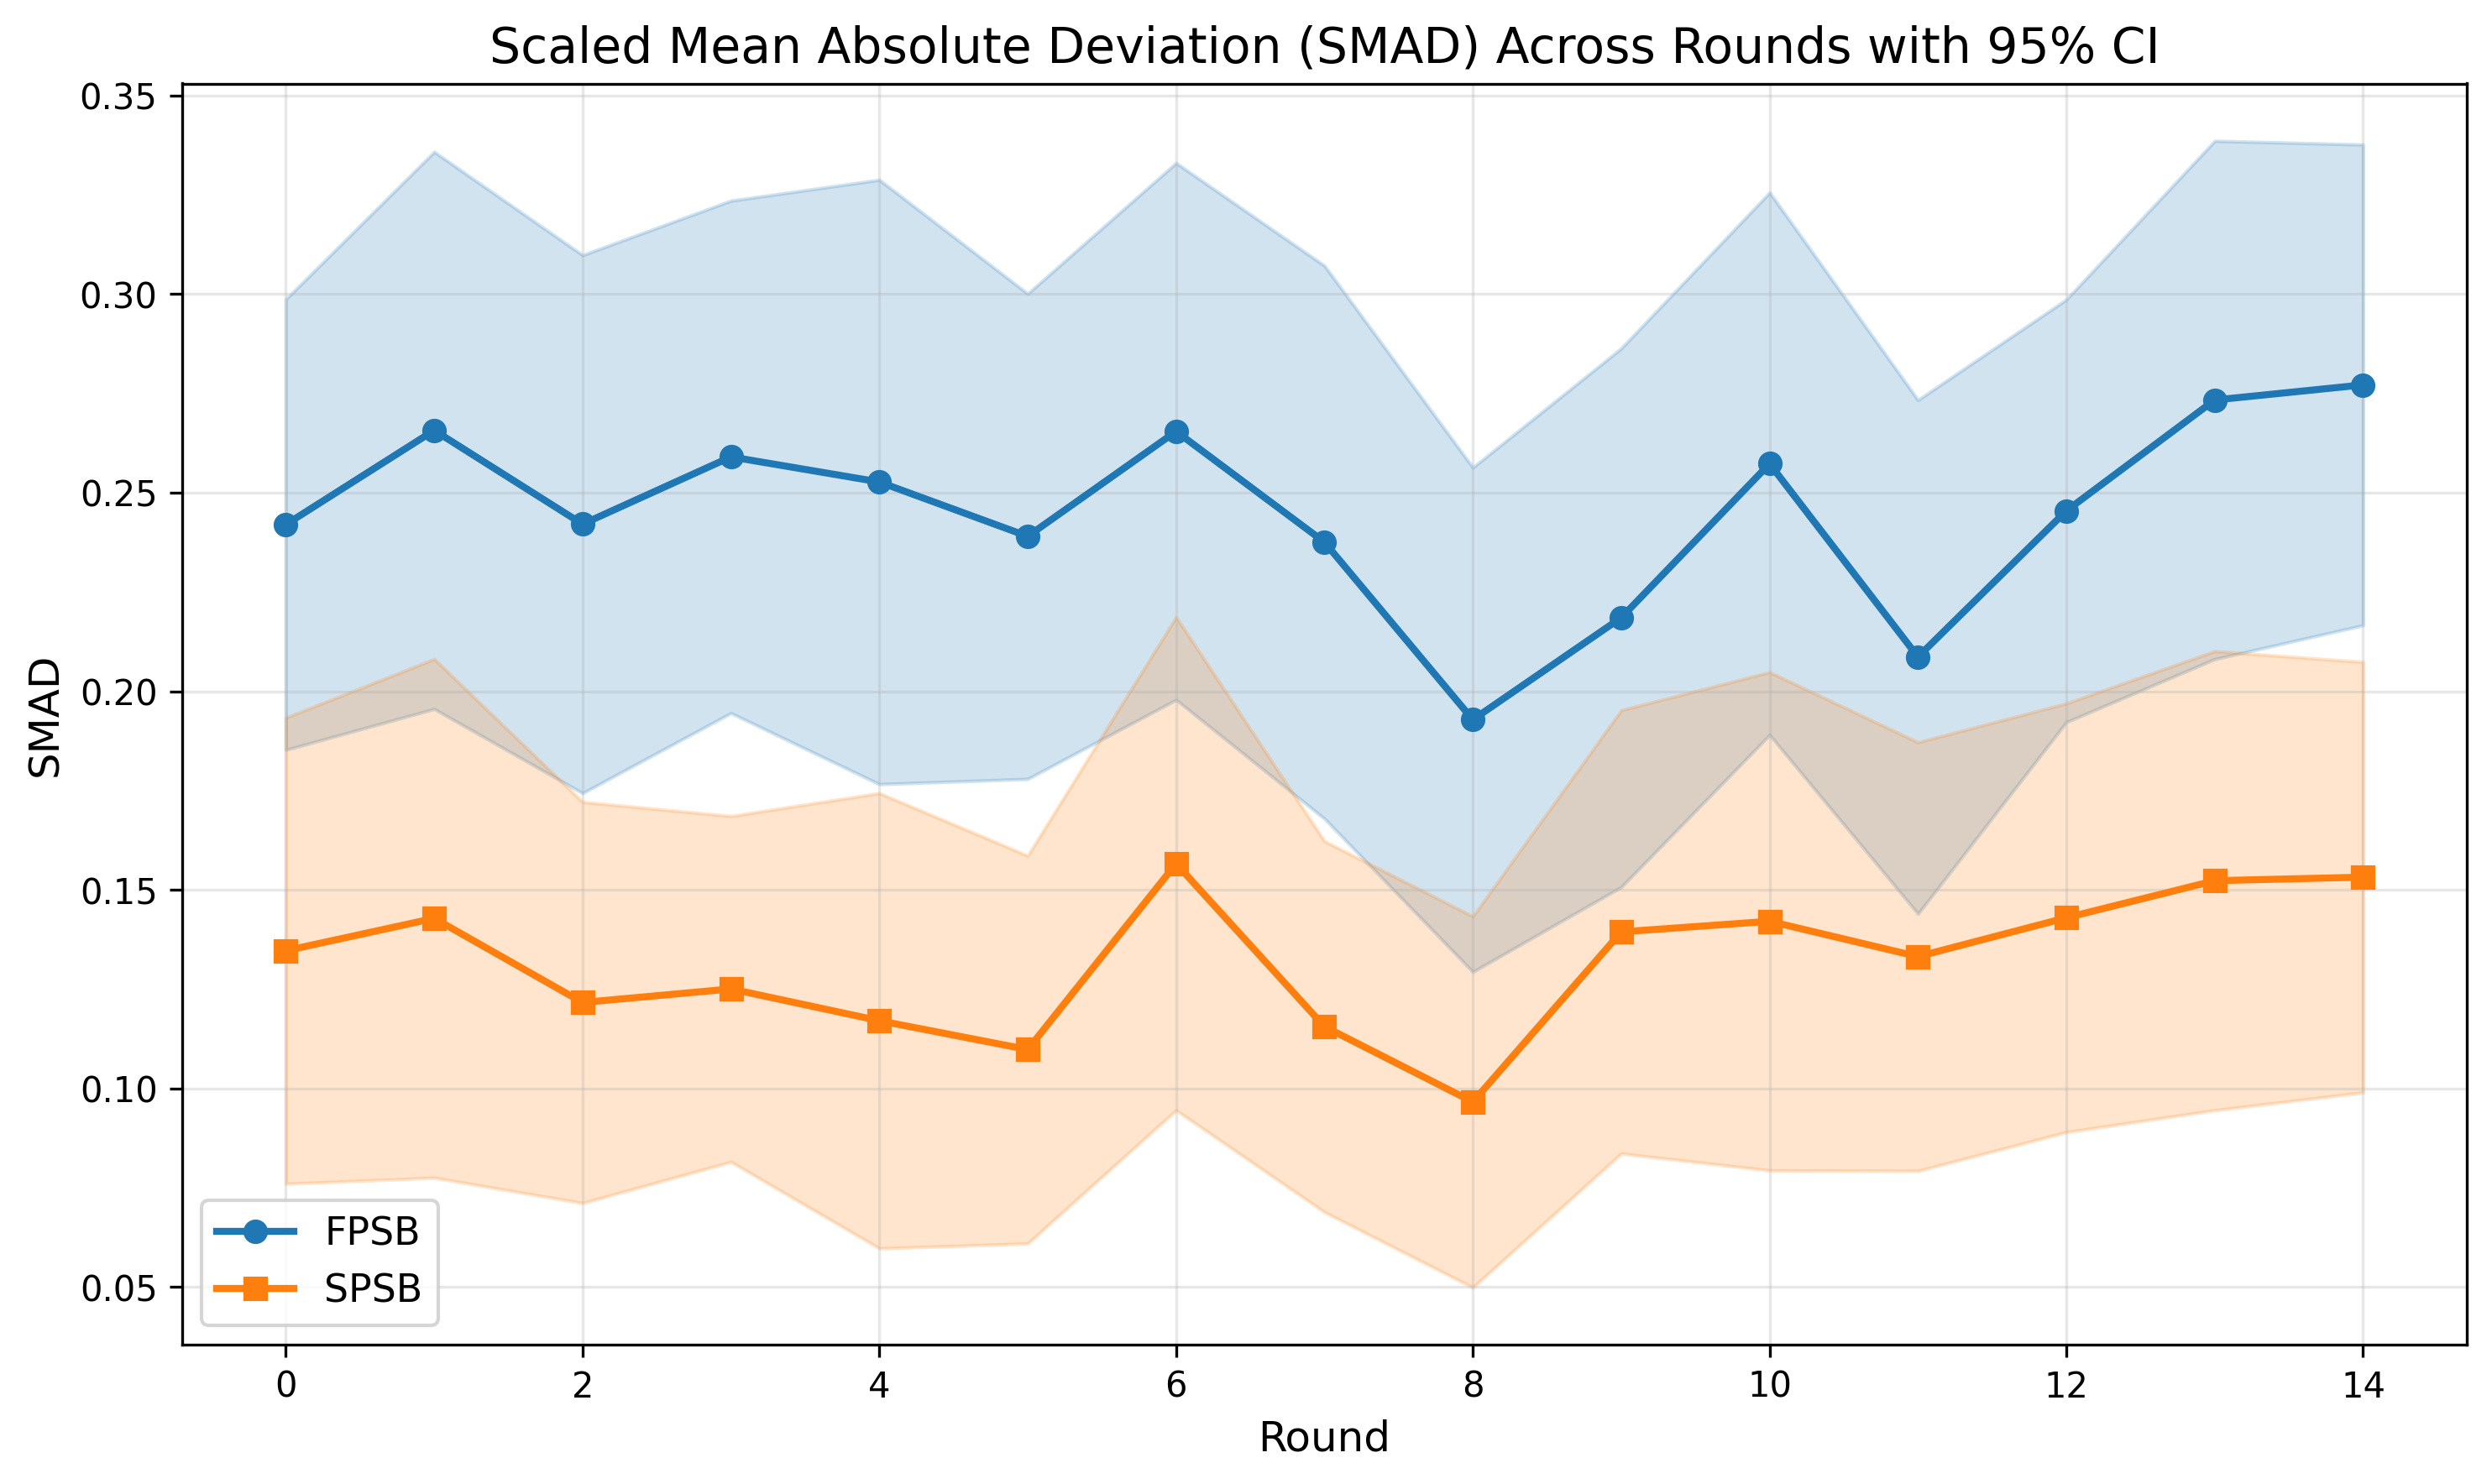
\includegraphics[scale=0.45]{smad_rounds.png}
    \caption{Repeated-play ablation: 15 consecutive rounds of first-price and second-price sealed-bid auctions with GPT-4o ($T=0.5$), where bidders observe the full outcome history of prior rounds. The y-axis is the scaled mean absolute deviation (SMAD) between actual and benchmark bids. Deviations show no trend in either format.}
    \label{fig:learning}
\end{figure}

% ---------------------------------------------------------------------------
% Appendix: Model and Temperature Ablations
% Source: writeup/contents/appendix.tex:238-328
% Fixes applied per plan §5: temperature text rewritten to match its own table
%   (§5.9); significance stars vs reconstructed humans removed (§5.8);
%   "Claude Sonnet 3.5" -> Claude 3.5 Haiku with config-verified footnote (§5.2);
%   Llama-3-8B as capability floor (§5.1). Frontier tier rewritten from
%   results/merged_ranking/auction_cells.csv + auction_cells_summary.md:
%   the old gpt-5-mini column was sourced to misattributed GPT-4o logs
%   (recovered_logs/experiment_logs_with_explanation/V10) and is removed.
%   2026-07-10: added tab:gemma-fidelity (E4) and tab:frontier-grid (the
%   10-cell lever grid on 4 frontier models: gpt-5-mini/gpt-5/claude-sonnet-5/
%   gemini-2.5-flash), all recomputed from results/merged_ranking/auction_cells.csv.
% ---------------------------------------------------------------------------
\section{Model and Temperature Ablations}\label{app:ablations}

This appendix reports the stability ablations referenced in Section~\ref{sec:validation}---varying the sampling temperature of the GPT-4o anchor, and varying the base model on the seven-format fidelity battery---together with a corrected accounting of the frontier tier (four reasoning models: gpt-5-mini, gpt-5, claude-sonnet-5, gemini-2.5-flash). Throughout, the human column is the moment-matched reconstruction of Section~\ref{sec:reconstruction}; consistent with the epistemic policy stated there, we report \emph{no} significance tests against reconstructed human benchmarks, because such tests would treat a model-based reconstruction as if it were sampled micro-data. Comparisons to the human column should be read qualitatively---rankings, directions, and orders of magnitude. \TODO{Attach Monte-Carlo percentile bands (and, once available, the parametric-bootstrap bands of Appendix~\ref{app:human}) to the human column in both tables (plan \S 5.8).}

\subsection{Varying temperature for the GPT-4o agent}

We vary GPT-4o's sampling temperature $T \in \{0.1, 0.5, 1.0\}$ across the seven fidelity-battery formats (Table~\ref{tab:temperature}; Figure~\ref{fig:ablations-temperature}). The temperature parameter controls the randomness of the model's outputs, with lower values producing more deterministic responses and higher values introducing more variability.

Two facts stand out. First, temperature effects are modest and, crucially, \emph{non-monotonic}: no temperature setting dominates. $T=0.1$ is strictly best in three of the seven formats (both ascending-clock formats and FPSB-CV) and strictly worst in three others (SPSB-IPV, SPSB-APV, and FPSB-IPV), with the remaining format (SPSB-CV) ordered $T=1.0 < T=0.1 < T=0.5$. Second, the pattern is consistent with temperature scaling the dispersion around the model's modal action rather than changing the underlying strategy: at $T=0.1$ the clock formats become exactly truthful (SMAD $= 0.00$) because near-deterministic decoding removes stochastic exits from an already-truthful modal policy, while in the sealed-bid formats the same determinism locks in the modal bias. We therefore retain $T=0.5$ throughout the paper as a \emph{convention}---it is the most common setting in LLM-based simulation \citep{horton2023large} and preserves comparability across models and with prior work---not because it is performance-optimal in any particular format. Temperature reappears in Section~\ref{sec:humans} as a candidate knob for \emph{cardinal} calibration to human levels; its effects there are likewise non-monotonic (on the rebuilt grid's normalization, SPSB-IPV SMAD is $15.1/8.9/13.2$ at $T=0.1/0.5/1.0$).

\begin{figure}[H]
    \centering
    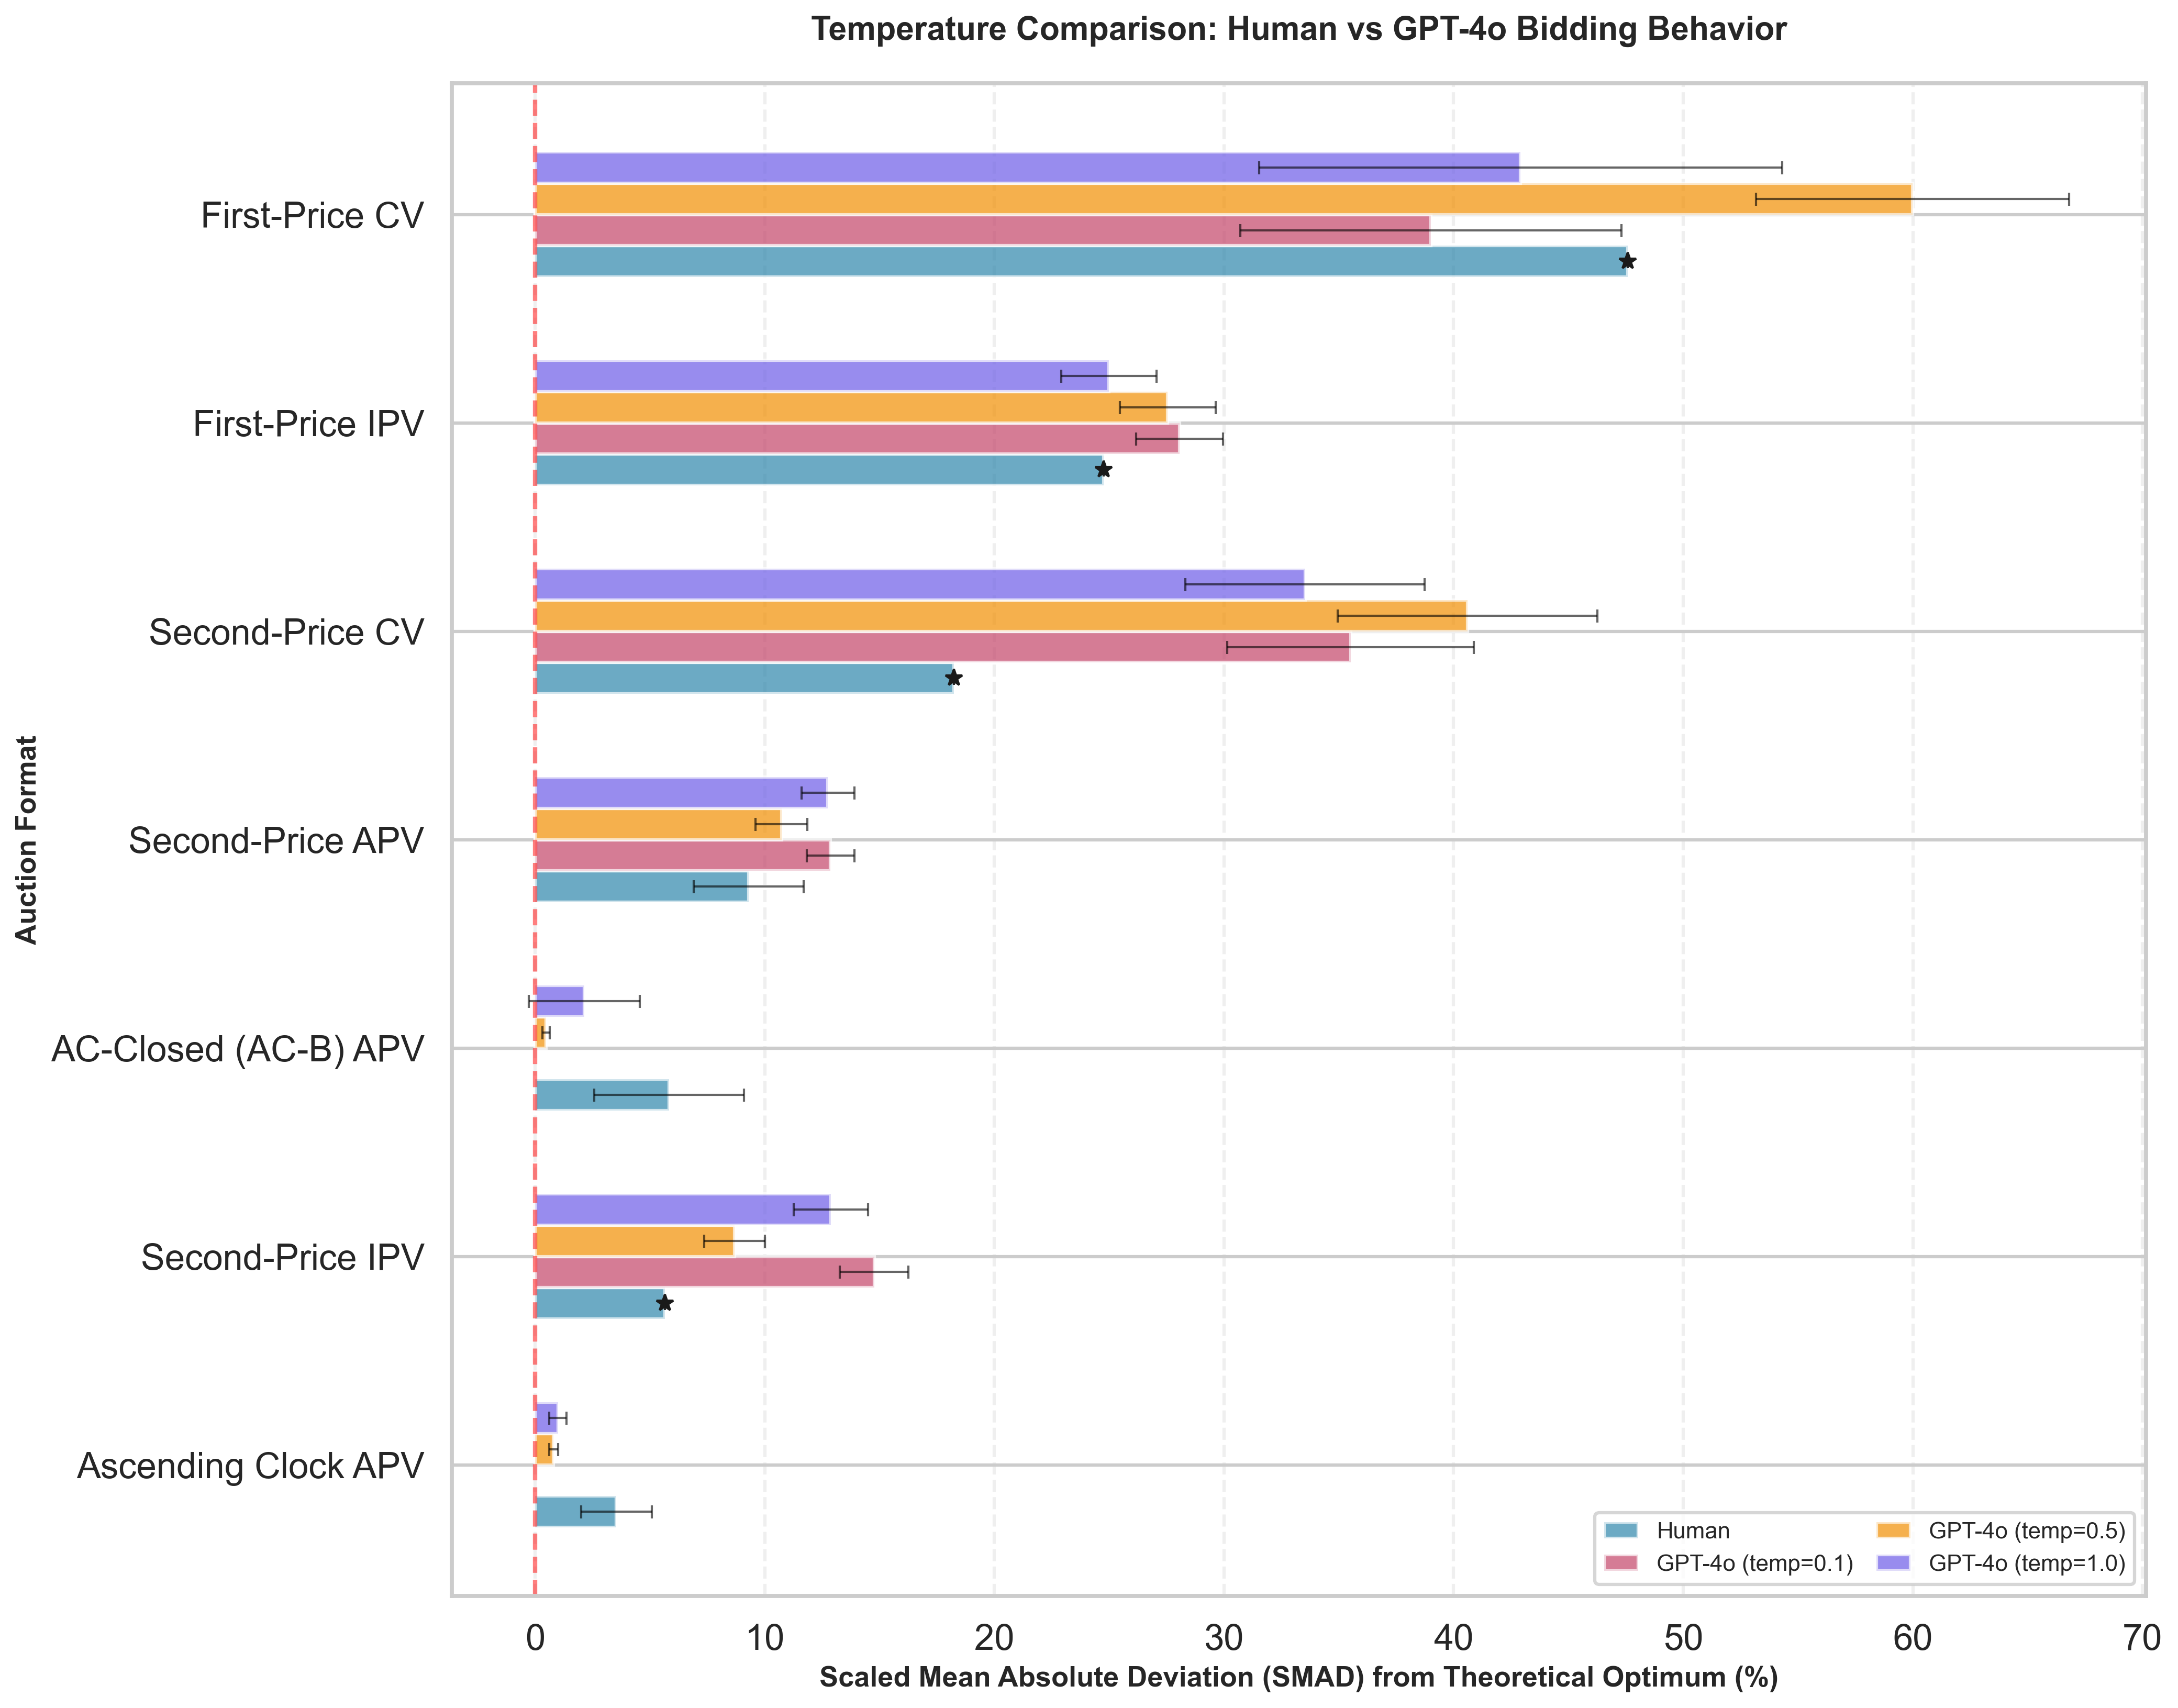
\includegraphics[scale=0.35]{appendix2_temperature_comparison.png}
    \caption{Comparison of the bidding behavior of reconstructed human participants and GPT-4o across three temperature settings ($T=0.1, 0.5, 1.0$) in seven auction formats. The horizontal bars represent the scaled mean absolute deviation (SMAD) from the theoretical benchmark, with error bars indicating 95\% confidence intervals (for the LLM cells only; see the text of this appendix for the human column's epistemic status).}
    \label{fig:ablations-temperature}
\end{figure}

\begin{table}[htbp]
\centering
\begin{tabular}{l|ccc}
\hline
Auction Format & $T=0.1$ & $T=0.5$ & $T=1.0$ \\
\hline
AC-B (closed clock), APV & 0.00 & 0.47 & 2.15 \\
AC (open clock), APV & 0.00 & 0.81 & 1.00 \\
SPSB, IPV & 14.77 & 8.69 & 12.89 \\
SPSB, APV & 12.87 & 10.73 & 12.75 \\
FPSB, CV & 39.00 & 59.99 & 42.92 \\
SPSB, CV & 35.51 & 40.60 & 33.53 \\
FPSB, IPV & 28.07 & 27.55 & 24.99 \\
\hline
\end{tabular}
\caption{Temperature effects on GPT-4o bidding behavior (SMAD, \%). SMAD = scaled mean absolute deviation from the theoretical benchmark. No temperature dominates: $T=0.1$ is strictly best in three formats and strictly worst in three others. Values use the legacy figure normalization ($\mathbb{E}[b^\star]=25$); the rebuilt cell-level grid normalizes by $24.5$, making values uniformly $\approx 2\%$ larger (e.g., SPSB-IPV $15.1/8.9/13.2$)---orderings and the non-monotonicity are unaffected.}
\label{tab:temperature}
\end{table}

\subsection{Varying the base model}

We repeat the seven-format fidelity battery, holding prompts fixed and $T=0.5$, for three models beyond the GPT-4o anchor: Claude 3.5 Haiku, Gemini 2.0 Flash, and Llama-3-8B-Instruct (an open-weight model).\footnote{Model identifiers: \texttt{claude-3-5-haiku-20241022}, \texttt{gemini-2.0-flash}, \texttt{Meta-Llama-3-8B-Instruct}, and, in the frontier tier below, \texttt{gpt-5-mini}, \texttt{gpt-5}, \texttt{claude-sonnet-5}, and \texttt{gemini-2.5-flash}. An earlier draft referred to the Anthropic model as ``Claude Sonnet 3.5''; the experiment configurations confirm that the runs stored under directories named \texttt{claude\_sonnet} (e.g., \texttt{robustness\_logs/V10/*claude\_sonnet*}) were in fact executed with \texttt{claude-3-5-haiku-20241022} (config-verified: \texttt{configs/clock/01\_06\_ascending\_clock\_apv\_claude\_sonnet.yaml}). The gpt-5-mini API ignores the temperature parameter.} Claude 3.5 Haiku and Gemini 2.0 Flash belong to the canonical model set of Section~\ref{sec:design}; Llama-3-8B-Instruct and the frontier reasoning models of Section~\ref{app:ablations-frontier} (treated separately below, because their data coverage differs) bracket the canonical set from below and above. Results appear in Table~\ref{tab:models} and Figure~\ref{fig:ablations-models}. The fourth canonical model, Gemma 27B, ran a separate six-format sealed-bid fidelity battery (Table~\ref{tab:gemma-fidelity}); we report it apart from Table~\ref{tab:models} because its cells are recomputed from the cell-level dataset (\path{results/merged_ranking/auction_cells.csv}, normalizer $\mathbb{E}[b^\star]=24.5$), a normalization that differs from the legacy figure scaling of the Claude/Gemini/Llama columns here (the same $\approx\!2\%$ offset flagged for Table~\ref{tab:temperature}), so the columns are not directly comparable cell-for-cell.

Llama-3-8B-Instruct serves as the \emph{capability floor}. It exhibits substantially degraded performance across all auction formats (mean SMAD $= 57.58\%$), exceeding the reconstructed human benchmark in six of seven formats---evidence that open-weight availability at small scale is not sufficient for competent strategic play, and that the canonical models sit well inside the band where design levers have room to operate. Claude 3.5 Haiku and Gemini 2.0 Flash behave broadly like the GPT-4o anchor: near-truthful in the clock formats, moderate deviations in the sealed-bid formats, and large deviations under common values. \TODO{The SPSB-IPV cells will be recomputed on the harmonized canonical dataset alongside signed means (plan E8, \S 5.3); the Claude SMAD/signed-mean contrast (worse absolute, best signed) is expected to persist and will be reported as such.} \TODO{Regenerate the figure asset \texttt{appendix2\_model\_comparison.png}: the legend of the current PNG carries the superseded ``Claude Sonnet 3.5'' label (see footnote in this appendix), and its gpt-5-mini series rests on the misattributed logs documented in Section~\ref{app:ablations-frontier} of this appendix and must be dropped or rebuilt from the genuine cells.}

\paragraph{Gemma 27B and the difficulty ordering.} The open-weight Gemma 27B model ran the sealed-bid fidelity battery in six formats ($K=30$ per cell; Table~\ref{tab:gemma-fidelity}). Its mean SMAD is $19.09\%$, between the canonical models and the Llama floor. The more instructive fact is not the level but the \emph{shape}: Gemma does \emph{not} reproduce the human difficulty ordering cleanly. In the human data the first-price format is much harder than the second-price dominant-strategy format---FPSB-IPV SMAD $24.76\%$ versus SPSB-IPV $5.65\%$, a ratio of $4.4$---and GPT-4o preserves that ordering ($27.55\%/8.69\% = 3.2$). Gemma nearly flattens it: $24.80\%$ in FPSB-IPV against $19.88\%$ in SPSB-IPV, a ratio of only $1.25$. It deviates almost as much in the format where truthful bidding is a dominant strategy as in the format where equilibrium requires shading, so the fidelity ordering that the auction ranking exploits is, in part, model-specific rather than a universal property of LLM bidders. The two ascending-clock cells are not yet run for Gemma (the per-tick clock harness is prohibitively slow, and reconciling the survey-style elicitation with the tick protocol is deferred to the native-key runs), so the clock rows of Table~\ref{tab:models} have no Gemma entry. \TODO{Gemma ascending-clock (AC and AC-B) cells pending native-key runs; survey-vs-tick harmonization deferred.}

\begin{table}[htbp]
\centering
\footnotesize
\begin{tabular}{l c c}
\hline
Auction Format & SMAD vs.\ value (\%) & Signed mean dev.\ (\$) \\
\hline
FPSB, IPV & 24.80 & $-5.89$ \\
TPSB, IPV & 23.31 & $-5.45$ \\
SPSB, IPV & 19.88 & $-4.87$ \\
SPSB, APV & 18.67 & $-4.57$ \\
FPSB, CV & 16.08 & $-2.57$ \\
SPSB, CV & 11.80 & $-1.44$ \\
\hline
\end{tabular}
\caption{Gemma 27B sealed-bid fidelity battery (SMAD, \% of $\mathbb{E}[b^\star]=24.5$; signed mean deviation from value in dollars). Recomputed from \texttt{results/merged\_ranking/auction\_cells.csv} (group \texttt{gemma27b}, $K=30$ per cell). Mean SMAD across the six formats is $19.09\%$. Gemma's FPSB-IPV/SPSB-IPV ratio is $1.25$, against $4.4$ for reconstructed humans and $3.2$ for GPT-4o: the model does not reproduce the human difficulty ordering, so the fidelity ordering is partly model-specific. The two ascending-clock cells (AC, AC-B) were not run for Gemma (per-tick harness too slow; survey-vs-tick harmonization pending native-key runs). CV deviations are relative to the private signal and carry no dominant-strategy benchmark.}
\label{tab:gemma-fidelity}
\end{table}

\begin{figure}[H]
    \centering
    
\includegraphics[scale=0.375]{appendix2_model_comparison.png}
    \caption{Comparison of the bidding behavior of reconstructed human participants and LLM agents across further foundation models in seven auction formats. The horizontal bars represent the scaled mean absolute deviation (SMAD) from the theoretical benchmark, with error bars indicating 95\% confidence intervals (LLM cells only). The gpt-5-mini series shown in the current asset is superseded (see the frontier discussion in the text; regeneration pending).}
    \label{fig:ablations-models}
\end{figure}

\begin{table}[htbp]
\centering
\begin{tabular}{l|c|ccc}
\hline
\multirow{2}{*}{Auction Format} & Human & Claude 3.5 & Gemini 2.0 & Llama-3-8B \\
 & (reconstr.) & Haiku & Flash & \\
\hline
FPSB, IPV & 24.76 & 24.09 & 27.05 & 38.16 \\
SPSB, IPV & 5.65 & 9.72 & 3.01 & 54.89 \\
AC-B (closed clock), APV & 5.83 & 0.00 & 1.26 & 67.00 \\
SPSB, APV & 9.31 & 9.58 & 8.02 & 53.08 \\
AC (open clock), APV & 3.54 & 5.74 & 0.00 & 104.10 \\
FPSB, CV & 47.59 & 54.07 & 59.50 & 53.68 \\
SPSB, CV & 18.23 & 27.19 & 30.89 & 32.27 \\
\hline
\end{tabular}
\caption{Fidelity battery across base models (SMAD, \%). SMAD = scaled mean absolute deviation from the theoretical benchmark. All models run at $T=0.5$. The human column is the moment-matched reconstruction of Section~\ref{sec:reconstruction}; no significance tests are reported against it because the reconstruction is model-based (see text and Appendix~\ref{app:human}). An earlier draft's gpt-5-mini column is removed: its source logs are GPT-4o (see the frontier subsection); the genuine gpt-5-mini cells appear in Table~\ref{tab:ablations-frontier}.}
\label{tab:models}
\end{table}

\subsection{The frontier tier: reasoning models do not uniformly dissolve the constraints}\label{app:ablations-frontier}

An earlier draft treated gpt-5-mini as a frontier \emph{ceiling} that plays near-optimally across a battery of sealed cells (mean SMAD $6.68\%$). That figure did not survive a provenance audit: the log tree from which it was computed (\path{recovered_logs/experiment_logs_with_explanation/V10/}) is GPT-4o in every run configuration---not gpt-5-mini---and shares most of its run identifiers with the anchor logs, so it is discarded. Two data sources now replace it. First, a genuine gpt-5-mini sealed-bid mechanism battery (Table~\ref{tab:ablations-frontier}), whose across-format mean SMAD \emph{against truthful value} is $19.09\%$ over the six robustness formats (or $16.6\%$ if the genuine clock cell below is included)---the $6.68\%$ figure is retired, not merely re-sourced. Second, and new to this draft, a full intervention grid run on four frontier models---gpt-5-mini, gpt-5, claude-sonnet-5, and gemini-2.5-flash (canonical identifiers; family \texttt{es\_v12} in \path{results/merged_ranking/auction_cells.csv})---which replaces the earlier claim that ``no gpt-5-mini intervention cells exist anywhere.'' The empty gpt-5-mini clock cells that motivated that claim are now explained: a configuration typo (\path{configs/clock/01_07_ascending_clock_apv_closed_gpt5mini.yaml} carried the invalid model id \texttt{gpt-4-mini}) suppressed the closed-clock robustness runs; with the typo fixed and the frontier battery's own \texttt{ascending\_clock\_closed} cell in hand ($K=50$, SMAD $1.25\%$), a genuine gpt-5-mini clock number exists and supersedes the empty cells.

\paragraph{The frontier intervention grid: truthful at baseline, but the backfire rungs retain teeth.} Table~\ref{tab:frontier-grid} reports the ten-cell lever grid across the four frontier models, entries recomputed from \path{auction_cells.csv} as mean deviation from value (dollars) with SMAD in parentheses. Three facts stand out. (i) \emph{All four frontier models are essentially exactly truthful at every sealed baseline}: mean deviations of $0.00$--$0.30$ and SMAD of $0$--$2.3\%$ across the sealed baseline cells, and the safety, payoff-tree, second-order-belief, and clock-framing description cells are inert (they land on the same $\approx\!0$ play, because there is no baseline error left to preserve). (ii) \emph{The menu restatement still breaks the frontier}, exactly the backfire the ranking predicts for its restatement rung: it moves claude-sonnet-5 catastrophically away from truthful play (mean deviation $-\$8.71$, SMAD $35.5\%$, $d=-3.8$, $p<10^{-58}$) and degrades gemini-2.5-flash (SMAD $2.3\% \to 9.1\%$, $p<10^{-8}$), while leaving gpt-5 and gpt-5-mini exactly truthful---the same sign-mixed, model-specific pattern the canonical menu cell shows, now with one model driven to a $35\%$ deviation. (iii) \emph{The true ascending clock makes frontier play \textbf{worse}, not better}: relative to their near-perfect sealed play, the closed clock raises claude-sonnet-5 from $0.27\%$ to $8.6\%$ SMAD and adds $+\$0.61$ (gpt-5) and $+\$0.28$ (gpt-5-mini) of mean deviation---an inversion of the canonical clock benefit, driven partly by the $\$0.5$-tick granularity of the clock grid interacting with models that otherwise bid value exactly. The extensive-form lever that helps bounded-rational agents is a small liability once the agent already plays the dominant strategy in the sealed format.

The gpt-5 cells carry reduced and uneven $K$: the model frequently omits the required response tags, and unparseable repetitions are dropped, so per-cell $n$ (in bids) ranges from $15$ to $150$ ($102$ for the SPSB baseline after its final top-up) (reported in Table~\ref{tab:frontier-grid}); the $n$ column should be read as a sample-size caveat; the run set is now frozen. gpt-5's DA cells were deliberately not run.

\TODO{gpt-5 intervention cells have reduced/uneven $K$ (15--150 parseable bids) from response-tag omissions; top up and re-freeze $n$ before the final draft. The frontier-battery runbook is \path{plan/FRONTIER_RUNBOOK.md}.}

The genuine cells sharpen, rather than remove, the paper's scope condition: \emph{frontier reasoning dissolves the bounded-rationality constraints where optimal play is textbook, and only there}. In the dominant-strategy format, gpt-5-mini is essentially perfect---mean deviation $-\$0.05$ (SMAD $0.2\%$) in SPSB-IPV and $-\$0.34$ ($1.4\%$) in SPSB-APV, truthful play at levels the canonical models reach only under the strongest levers. In FPSB-IPV, its bids sit $\$8.53$ below value on average, i.e., almost exactly on the risk-neutral equilibrium shading rule $\frac{n-1}{n}v$ (mean deviation from the RNE benchmark $+\$0.002$; SMAD against RNE $0.1\%$)---it applies the textbook formula.\footnote{The cell-level data (\path{results/merged_ranking/auction_cells.csv}) report deviations against both truthful bidding and each format's own equilibrium benchmark; against truthful bidding the FPSB cell reads SMAD $34.8\%$, which measures correct equilibrium shading, not error.} But in the \emph{third-price} format, where the equilibrium bid $\frac{n-1}{n-2}v$ exceeds value and no textbook formula is rehearsed in training corpora, the frontier model fails: with $n=3$ it overbids value by $+\$14.76$ on average yet remains $\$10.87$ \emph{below} the equilibrium bid $2v$ (SMAD $60.2\%$ against truthful play, $22.5\%$ against the equilibrium benchmark); with $n=5$ the same pattern appears at smaller scale ($+\$4.39$ above value, $\$4.11$ below the $\frac{4}{3}v$ equilibrium). It recognizes that third-price rules reward aggression but cannot compute how much. The common-value cells show similarly dispersed behavior (deviations relative to the private signal $-\$2.91$ and $-\$2.60$, with wide spreads; descriptive only, as no dominant-strategy benchmark exists).

The implication for the main text is a two-sided scope condition. On one side, at the frontier the gaps that the design levers close have vanished \emph{in the strategy-proof formats the ranking studies}---confirmed directly by the intervention grid of Table~\ref{tab:frontier-grid}, in which every safety, tree, and belief cell is inert because there is no baseline error left to preserve---which is why reasoning models are excluded from the main treatment grid, and why the ranking's practical relevance turns on deployed agent fleets occupying the sub-frontier regime for cost reasons (Section~\ref{sec:discussion}). On the other side, the third-price cells show that frontier reasoning does \emph{not} uniformly dissolve bounded rationality: where the required strategic computation is non-obvious, even the frontier model deviates by more than any canonical model deviates in second price. And the frontier grid shows that the backfire rungs keep their teeth: the menu restatement drives claude-sonnet-5 to a $35\%$ deviation and the true clock inverts into a small liability (Table~\ref{tab:frontier-grid}). Whether the levers of Section~\ref{sec:ranking} would repair a frontier model's third-price play---a format the grid does not yet cover---remains the natural next question.

\begin{table}[htbp]
\centering
\footnotesize
\begin{tabular}{l c c c c c}
\hline
Format & $n$ bids & Mean dev.\ vs.\ value (\$) & SMAD vs.\ $v$ (\%) & Mean dev.\ vs.\ $b^\star$ (\$) & SMAD vs.\ $b^\star$ (\%) \\
\hline
SPSB, IPV & 87 & $-0.05$ \([-0.15, 0.00]\) & 0.2 & $-0.05$ & 0.2 \\
SPSB, APV & 87 & $-0.34$ \([-0.53, -0.18]\) & 1.4 & $-0.34$ & 1.4 \\
FPSB, IPV & 87 & $-8.53$ \([-9.33, -7.74]\) & 34.8 & $+0.00$ & 0.1 \\
TPSB, IPV ($n{=}3$) & 87 & $+14.76$ \([12.32, 17.28]\) & 60.2 & $-10.87$ & 22.5 \\
TPSB, IPV ($n{=}5$) & 130 & $+4.39$ \([2.83, 6.19]\) & 26.5 & $-4.11$ & 18.2 \\
FPSB, CV & 90 & $-2.91$ \([-5.19, -0.74]\) & 36.6 & --- & --- \\
SPSB, CV & 90 & $-2.60$ \([-4.93, -0.37]\) & 36.9 & --- & --- \\
\hline
\end{tabular}
\caption{Genuine gpt-5-mini sealed-bid mechanism cells (\texttt{robustness\_logs/*\_gpt5mini}; brackets are bootstrap 95\% CIs on the mean deviation vs.\ value). $b^\star$ is each format's own benchmark: truthful bidding in SPSB, $\frac{n-1}{n}v$ in FPSB, $\frac{n-1}{n-2}v$ in TPSB. CV deviations are relative to the private signal and carry no dominant-strategy benchmark. The gpt-5-mini ascending-clock and intervention cells appear separately in Table~\ref{tab:frontier-grid} (frontier grid).}
\label{tab:ablations-frontier}
\end{table}

\begin{table}[htbp]
\centering
\footnotesize
\setlength{\tabcolsep}{4.5pt}
\begin{tabular}{ll cccc}
\toprule
& & \multicolumn{4}{c}{Mean dev.\ vs.\ value, \$ (SMAD vs.\ $v$, \%)} \\
\cmidrule(lr){3-6}
Lever grid cell & Family & gpt-5-mini & gpt-5$^{\dagger}$ & claude-sonnet-5 & gemini-2.5-flash \\
\midrule
\multicolumn{6}{l}{\emph{Sealed baselines}} \\
SPSB, IPV baseline & --- & $0.00$ ($0.0$) & $0.00$ ($0.0$; $n{=}102$) & $-0.07$ ($0.3$) & $-0.30$ ($2.3$) \\
Contingent baseline (axis 1) & --- & $0.00$ ($0.0$) & $0.00$ ($0.0$; $n{=}69$) & $0.00$ ($0.0$) & $-0.16$ ($0.9$) \\
Beliefs baseline (axis 3) & --- & $0.00$ ($0.0$) & $0.00$ ($0.0$; $n{=}45$) & $0.00$ ($0.0$) & $0.00$ ($0.2$) \\
\addlinespace
\multicolumn{6}{l}{\emph{Description / scaffold levers}} \\
Payoff Safety & B2 & $0.00$ ($0.0$) & $0.00$ ($0.0$; $n{=}132$) & $0.00$ ($0.0$) & $0.00$ ($0.0$) \\
Payoff Tree & C1 & $0.00$ ($0.0$) & $0.00$ ($0.0$; $n{=}72$) & $0.00$ ($0.0$) & $-0.01$ ($0.5$) \\
Second-order beliefs & C3 & $0.00$ ($0.0$) & $0.00$ ($0.0$; $n{=}54$) & $0.00$ ($0.0$) & $-0.07$ ($0.5$) \\
Clock framing (text) & B3 & $0.00$ ($0.0$; $n{=}36$) & $0.00$ ($0.0$; $n{=}27$) & $0.00$ ($0.0$) & $-0.29$ ($1.2$) \\
Two-stage exit description & B3 & $0.00$ ($0.0$) & $0.00$ ($0.0$; $n{=}87$) & $0.00$ ($0.0$) & $-0.04$ ($0.2$) \\
\textbf{Menu restatement} & B1 & $0.00$ ($0.0$) & $0.00$ ($0.0$; $n{=}15$) & $\mathbf{-8.71}$ ($\mathbf{35.5}$) & $-2.19$ ($9.1$) \\
\addlinespace
\multicolumn{6}{l}{\emph{Extensive form}} \\
\textbf{Ascending clock (AC-B)} & A & $+0.28$ ($1.3$) & $+0.61$ ($2.7$) & $-2.08$ ($8.6$) & $-0.16$ ($0.8$) \\
\bottomrule
\end{tabular}
\caption{Frontier intervention grid: the ten-cell lever grid on four frontier models, recomputed from \texttt{results/merged\_ranking/auction\_cells.csv} (family \texttt{es\_v12}; canonical model ids). Entries are mean deviation from value in dollars, with SMAD (\% of $\mathbb{E}[b^\star]=24.5$) in parentheses; each cell is $K=50$ ($n\approx 150$ bids) except as noted. All four models are near-exactly truthful at every sealed baseline, and the safety, tree, belief, and clock-framing description cells are inert (no baseline error remains to preserve). Two backfire rungs retain teeth: the \emph{menu restatement} breaks claude-sonnet-5 (mean dev $-\$8.71$, SMAD $35.5\%$, Cohen's $d=-3.8$, $p<10^{-58}$) and degrades gemini-2.5-flash (SMAD $2.3\%\!\to\!9.1\%$, $p<10^{-8}$) while leaving gpt-5/gpt-5-mini exactly truthful; and the true \emph{ascending clock} makes frontier play \emph{worse} than sealed (claude-sonnet-5 SMAD $0.3\%\!\to\!8.6\%$; gpt-5 $+\$0.61$ and gpt-5-mini $+\$0.28$ mean deviation), partly a \$0.5-tick granularity artifact. $^{\dagger}$gpt-5 cells have reduced and uneven parseable $K$ (the model often omits response tags; unparseable repetitions are dropped): per-cell $n$ in bids is noted in the column---read $n$ as a caveat; the run set is frozen. gpt-5's DA cells were deliberately not run.}
\label{tab:frontier-grid}
\end{table}

% ---------------------------------------------------------------------------
% Appendix: Preference-Framing Interventions (Family D)
% Source: Engineering_simplicity/contents/appendix.tex:442-502 (reuse, adapted)
% Role in merged paper: Family-D rungs at the bottom of the ranking (plan §4).
% Figures resolve via \graphicspath to ../Engineering_simplicity/plots/.
% Known fixes applied: grammar in the risk-priming sentence; "main text"
% cross-references retargeted to the merged section labels.
% ---------------------------------------------------------------------------
\section{Preference-Framing Interventions}\label{app:prospect}

In addition to the extensive-form, description, and reasoning-scaffold levers reported in the main text (Families A--C of Section~\ref{sec:framework}), we test a separate family of interventions---Family~D---inspired by prospect theory \citep{kahneman1979prospect} and behavioral departures from expected utility theory. These interventions do not scaffold strategic reasoning; instead, they reframe the payoff structure to test whether LLMs exhibit sensitivity to framing effects, loss aversion, the endowment effect, and risk attitudes. Because truthful play is a dominant strategy in both of our environments regardless of risk preferences, none of these framings should move a rational agent; expectations-based loss aversion has nonetheless been proposed as an explanation for seemingly dominated choices by humans in strategy-proof matching mechanisms \citep{dreyfuss2022expectations}, which makes the family a natural placebo-adjacent battery for our testbed. We test these framings across both domains (SPSB auctions and direct DA) with the same four model families as the main grid (GPT-4o, Claude 3.5 Haiku, Gemini 2.0 Flash, Gemma 27B). In the assembled ranking of Section~\ref{sec:ranking-synthesis}, Family~D populates the bottom rungs: the risk-averse persona is the worst lever we measure, with provisional preservation index $\rho \approx -0.76$ in auctions and $\rho \approx -3.5$ in DA (Table~\ref{tab:ranking}).

\TODO{All Family-D cells below are point estimates from the ES runs (auction cells: IPV sealed-bid grid, seed 1299, $K=50$ auctions per cell; DA cells: 50 market instances per cell). E6 statistics (SEs, MW/Welch tests, Cohen's $d$, bootstrap CIs on $\rho$) and the harmonized re-runs (plan E3/E8) are pending; report SMAD alongside signed means when recomputed.}

\subsection{Loss aversion and framing effects}\label{app:prospect-loss}

We test five variants that reframe the payoff description while holding the mechanism and underlying payoffs constant:

\begin{itemize}
    \item \emph{Gain Frame}: Presents all outcomes as gains from zero (``you cannot lose money---you can only gain'').
    \item \emph{Loss Frame}: Endows the agent with an initial amount equal to their maximum possible value, then presents outcomes as losses from this reference point (``Think carefully about what you might lose'').
    \item \emph{Mixed Frame}: Explicitly decomposes each outcome into a GAIN component and a LOSE component, asking the agent to weigh both.
    \item \emph{Endowment}: Gives the agent an initial endowment and frames payment as a deduction ``from your endowment,'' targeting the endowment effect.
    \item \emph{WTA/WTP}: Asks the agent to compare their willingness-to-accept (selling price) with their willingness-to-pay (buying price), invoking the classic WTA--WTP gap.
\end{itemize}

\begin{figure}[H]
    \centering
    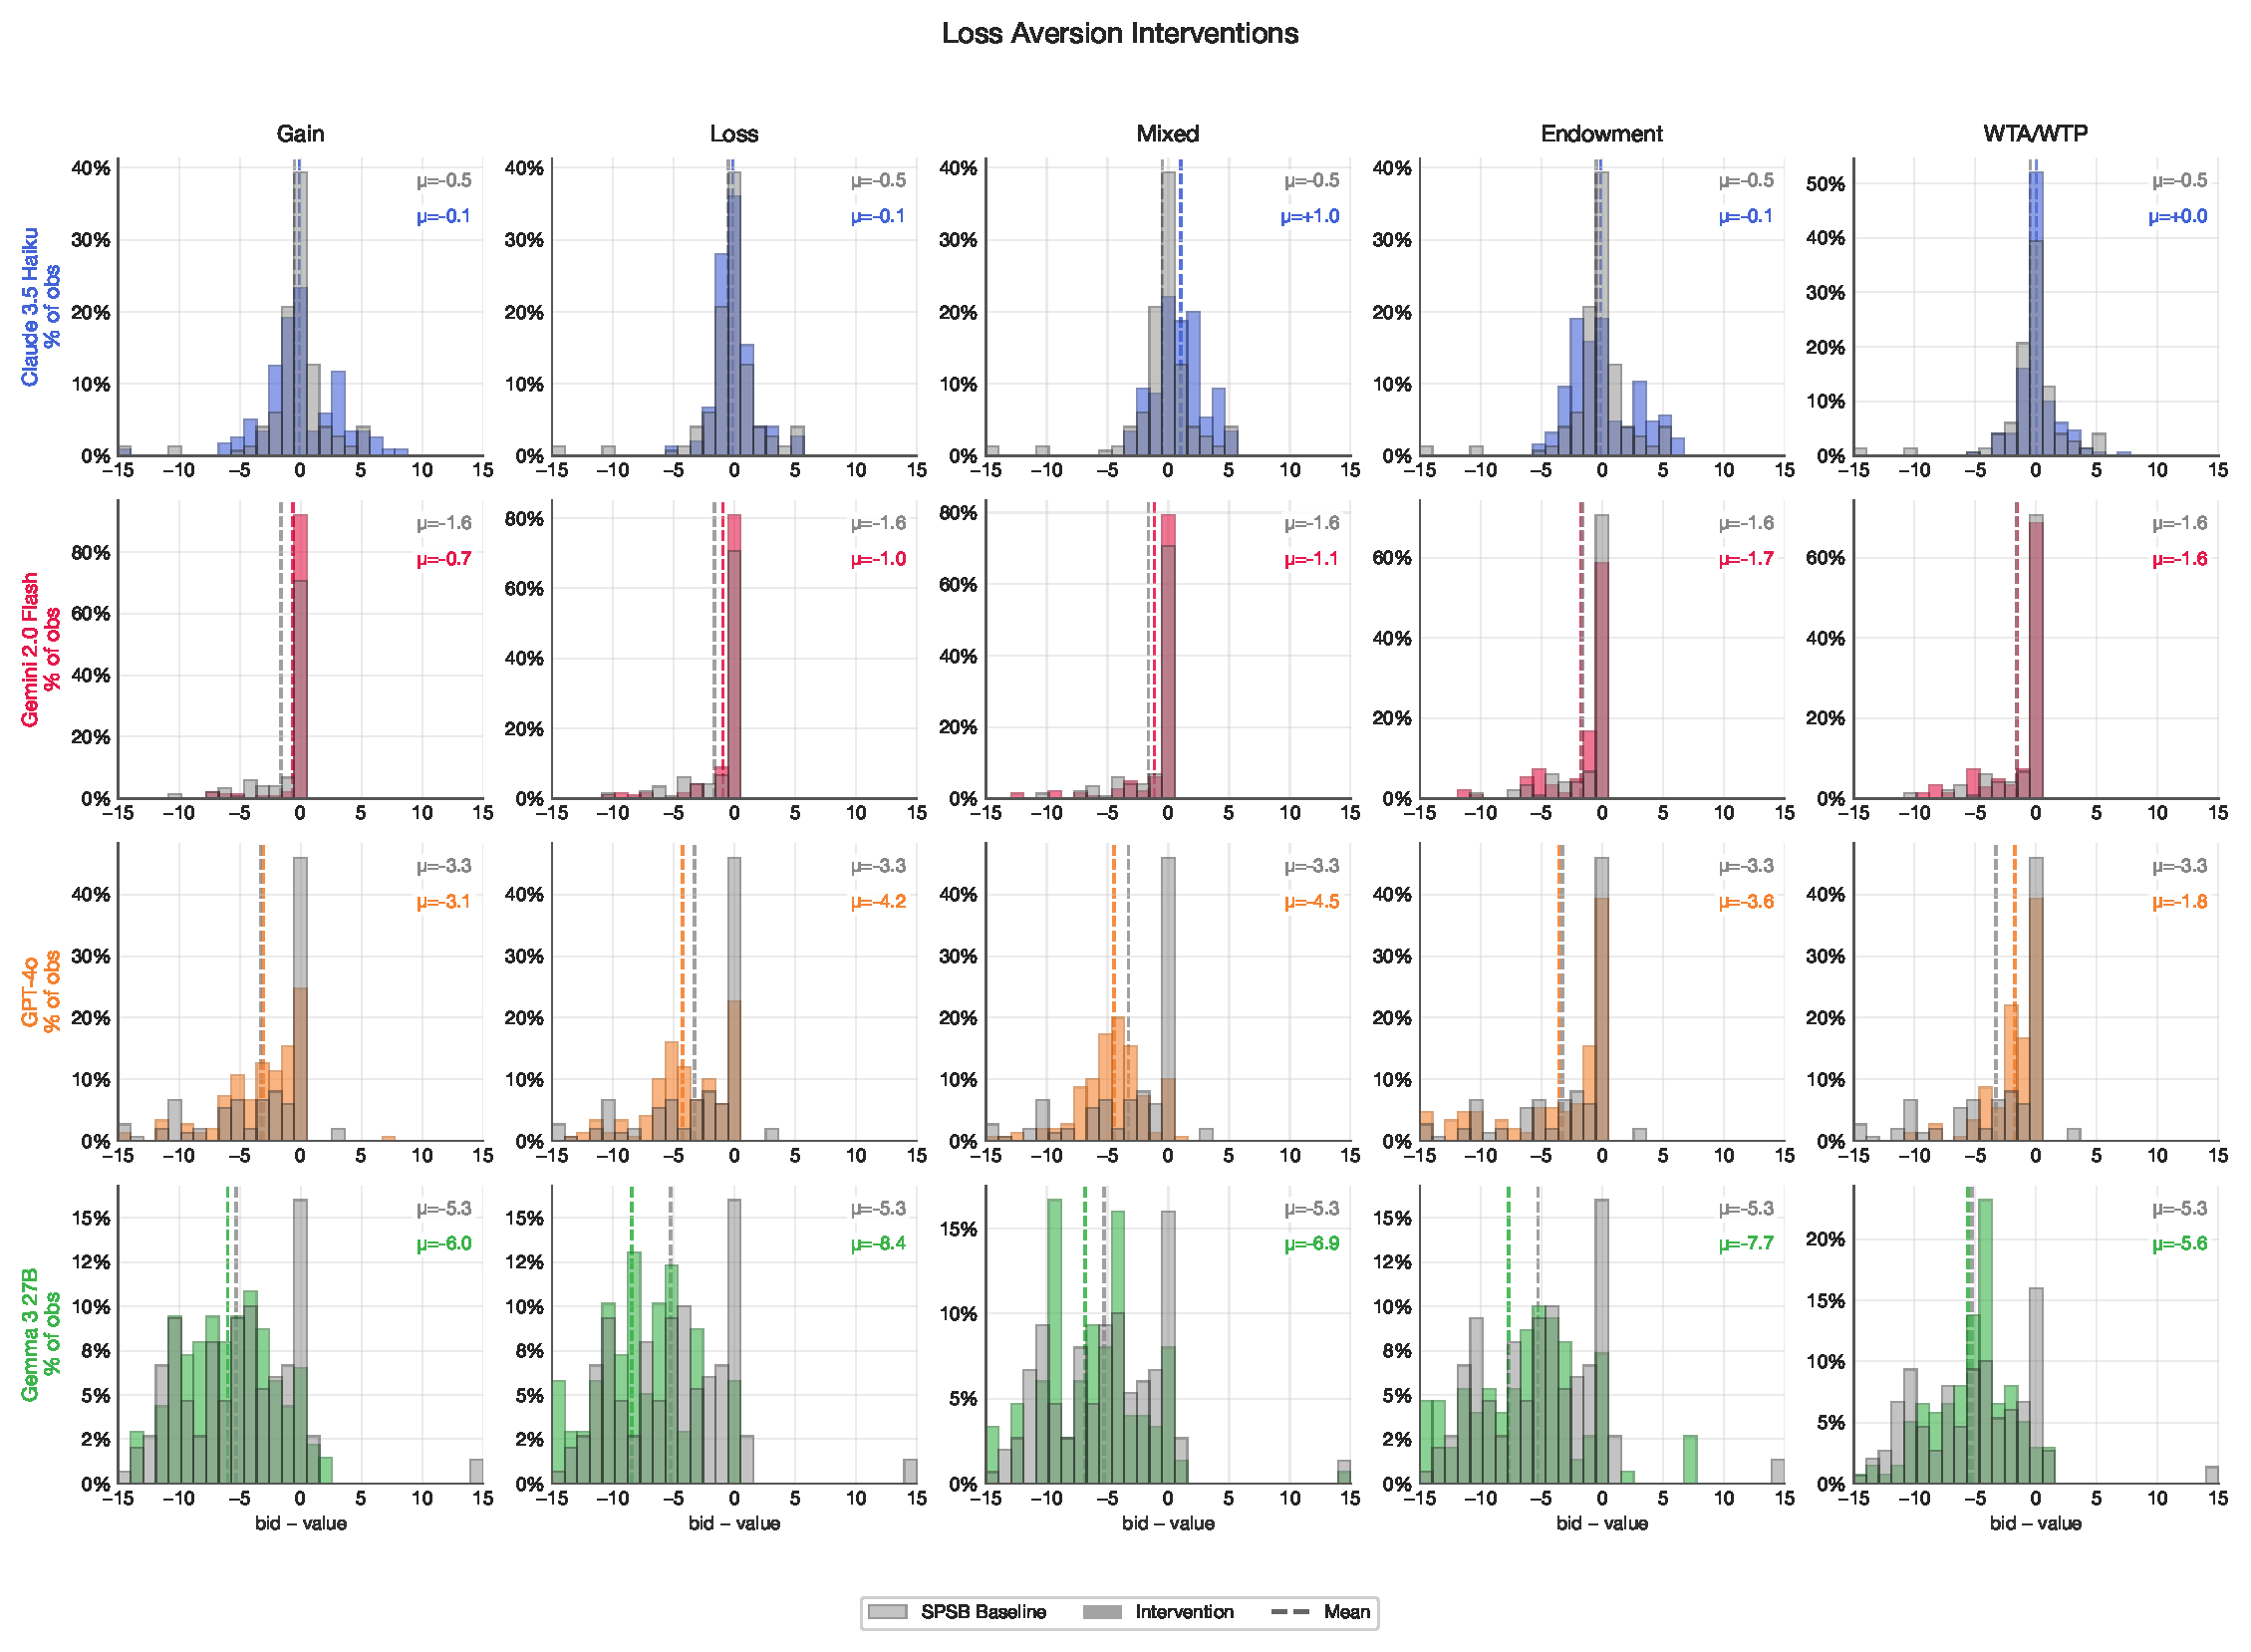
\includegraphics[width=\textwidth]{appendix_loss_aversion_auctions.pdf}
    \caption{Loss-aversion and framing interventions in SPSB auctions (mean bid deviation from value, \$). Baseline SPSB in gray, intervention in color; dashed lines indicate means. None of the framing interventions consistently improve play relative to the SPSB baseline ($\mu = -2.67$). The loss frame ($\mu = -3.44$) and endowment ($\mu = -3.40$) worsen underbidding, while the gain frame ($\mu = -2.51$) and WTA/WTP ($\mu = -2.17$) show modest, inconsistent effects.}
    \label{fig:prospect-loss-auctions}
\end{figure}

\begin{figure}[H]
    \centering
    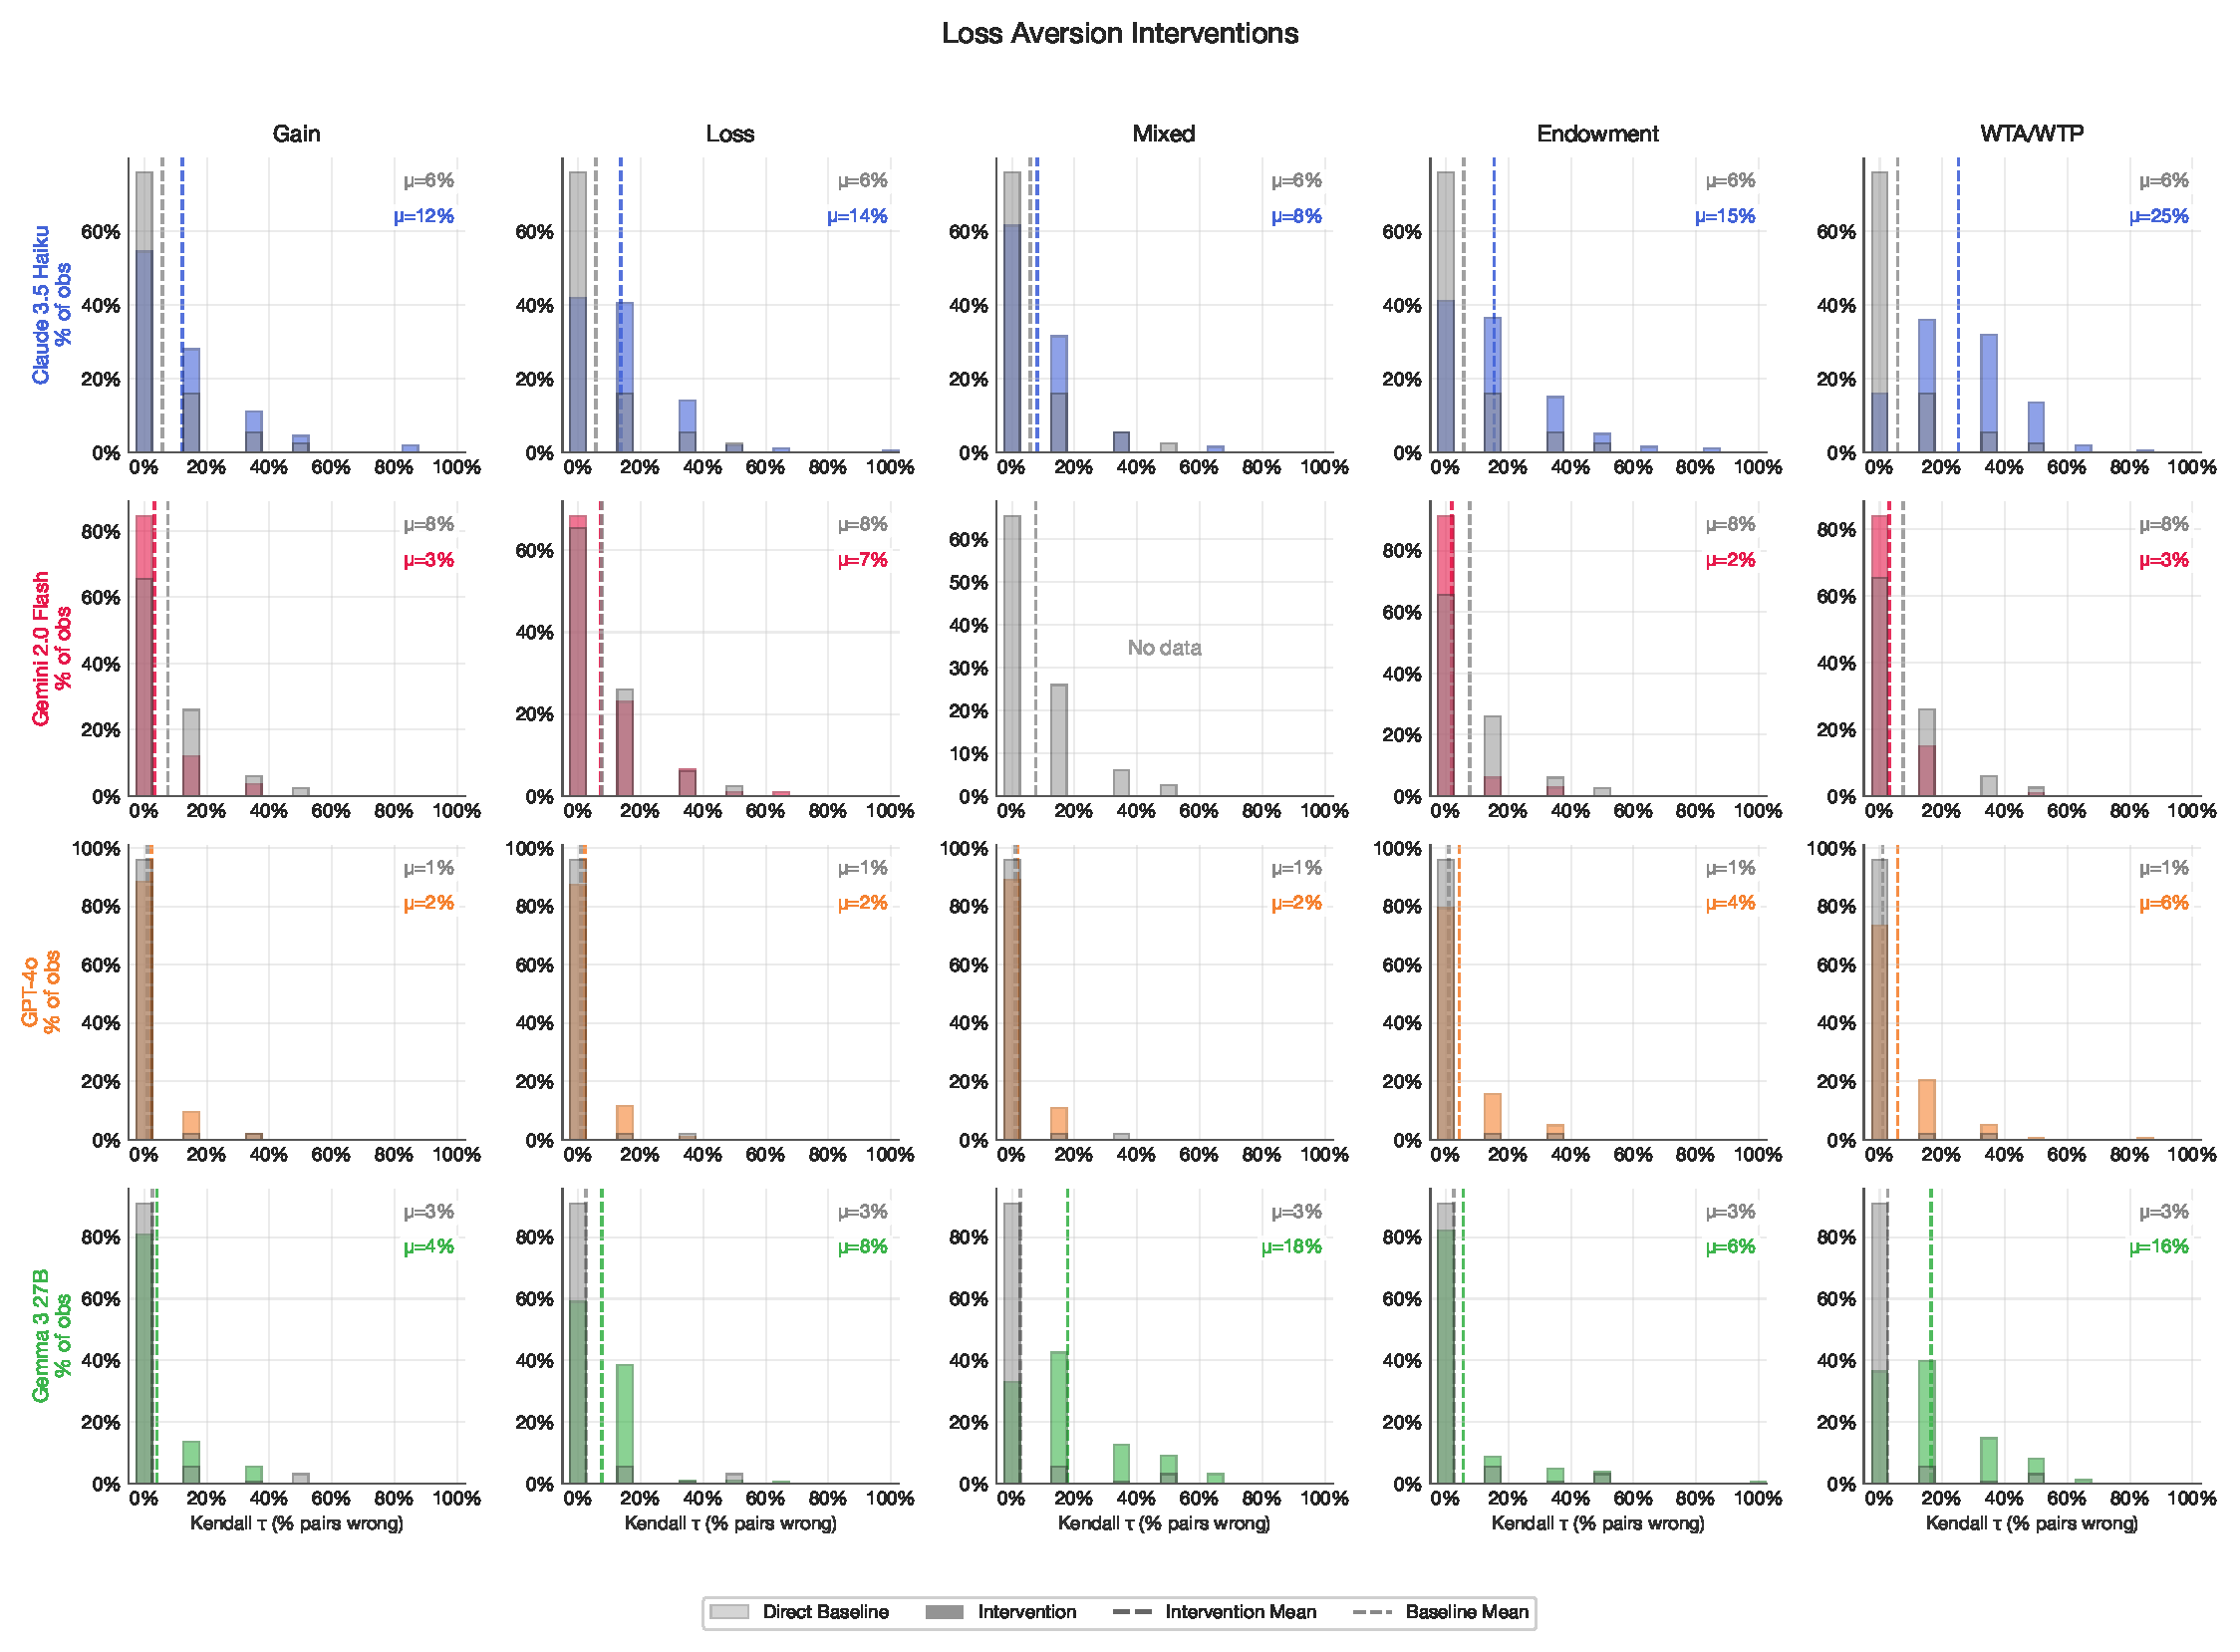
\includegraphics[width=\textwidth]{appendix_loss_aversion_da.pdf}
    \caption{Loss-aversion and framing interventions in deferred acceptance (mean normalized Kendall-$\tau$ error, \%). Baseline direct DA in gray, intervention in color. The results are noisy and largely negative: most framing interventions worsen play relative to the baseline ($\mu = 4.2\%$), with WTA/WTP producing the worst outcomes ($\mu \approx 12.6\%$ across models with data). Claude 3.5 Haiku is particularly sensitive to these framings.}
    \label{fig:prospect-loss-da}
\end{figure}

In auctions, the framing interventions do not produce consistent improvements. The loss frame and endowment interventions worsen underbidding (overall means of $\mu = -3.44$ and $-3.40$, compared to the SPSB baseline of $-2.67$), opposite to what a naive application of loss aversion would predict. The gain frame and WTA/WTP interventions produce small, model-dependent effects. In DA, the interventions are uniformly harmful, with WTA/WTP and endowment producing the largest increases in error.

The overall picture is that prospect-theoretic framings do not improve play---and often worsen it. This contrasts with the levers in the strong tiers of the ranking (Section~\ref{sec:ranking}): contingent-reasoning scaffolds and safety-exposing mechanism descriptions produce large, consistent improvements. The difference is informative: the cognitive barrier in these mechanisms is not about how payoffs are framed, but about understanding the mechanism's strategic structure.

\subsection{Risk-preference personas}\label{app:prospect-risk}

We also test whether assigning explicit risk attitudes to LLMs changes behavior. Each intervention instructs the model to adopt a calibrated risk preference via a concrete coin-toss example (full persona text in Appendix~\ref{app:prompts}):

\begin{itemize}
    \item \emph{Risk Averse}: ``You would only pay \$4 for a coin toss worth \$0 or \$10 (expected value \$5).''
    \item \emph{Risk Neutral}: ``You would pay \$5 for a coin toss worth \$0 or \$10.''
    \item \emph{Risk Seeking}: ``You would pay \$6 for a coin toss worth \$0 or \$10 (expected value \$5).''
\end{itemize}

\begin{figure}[H]
    \centering
    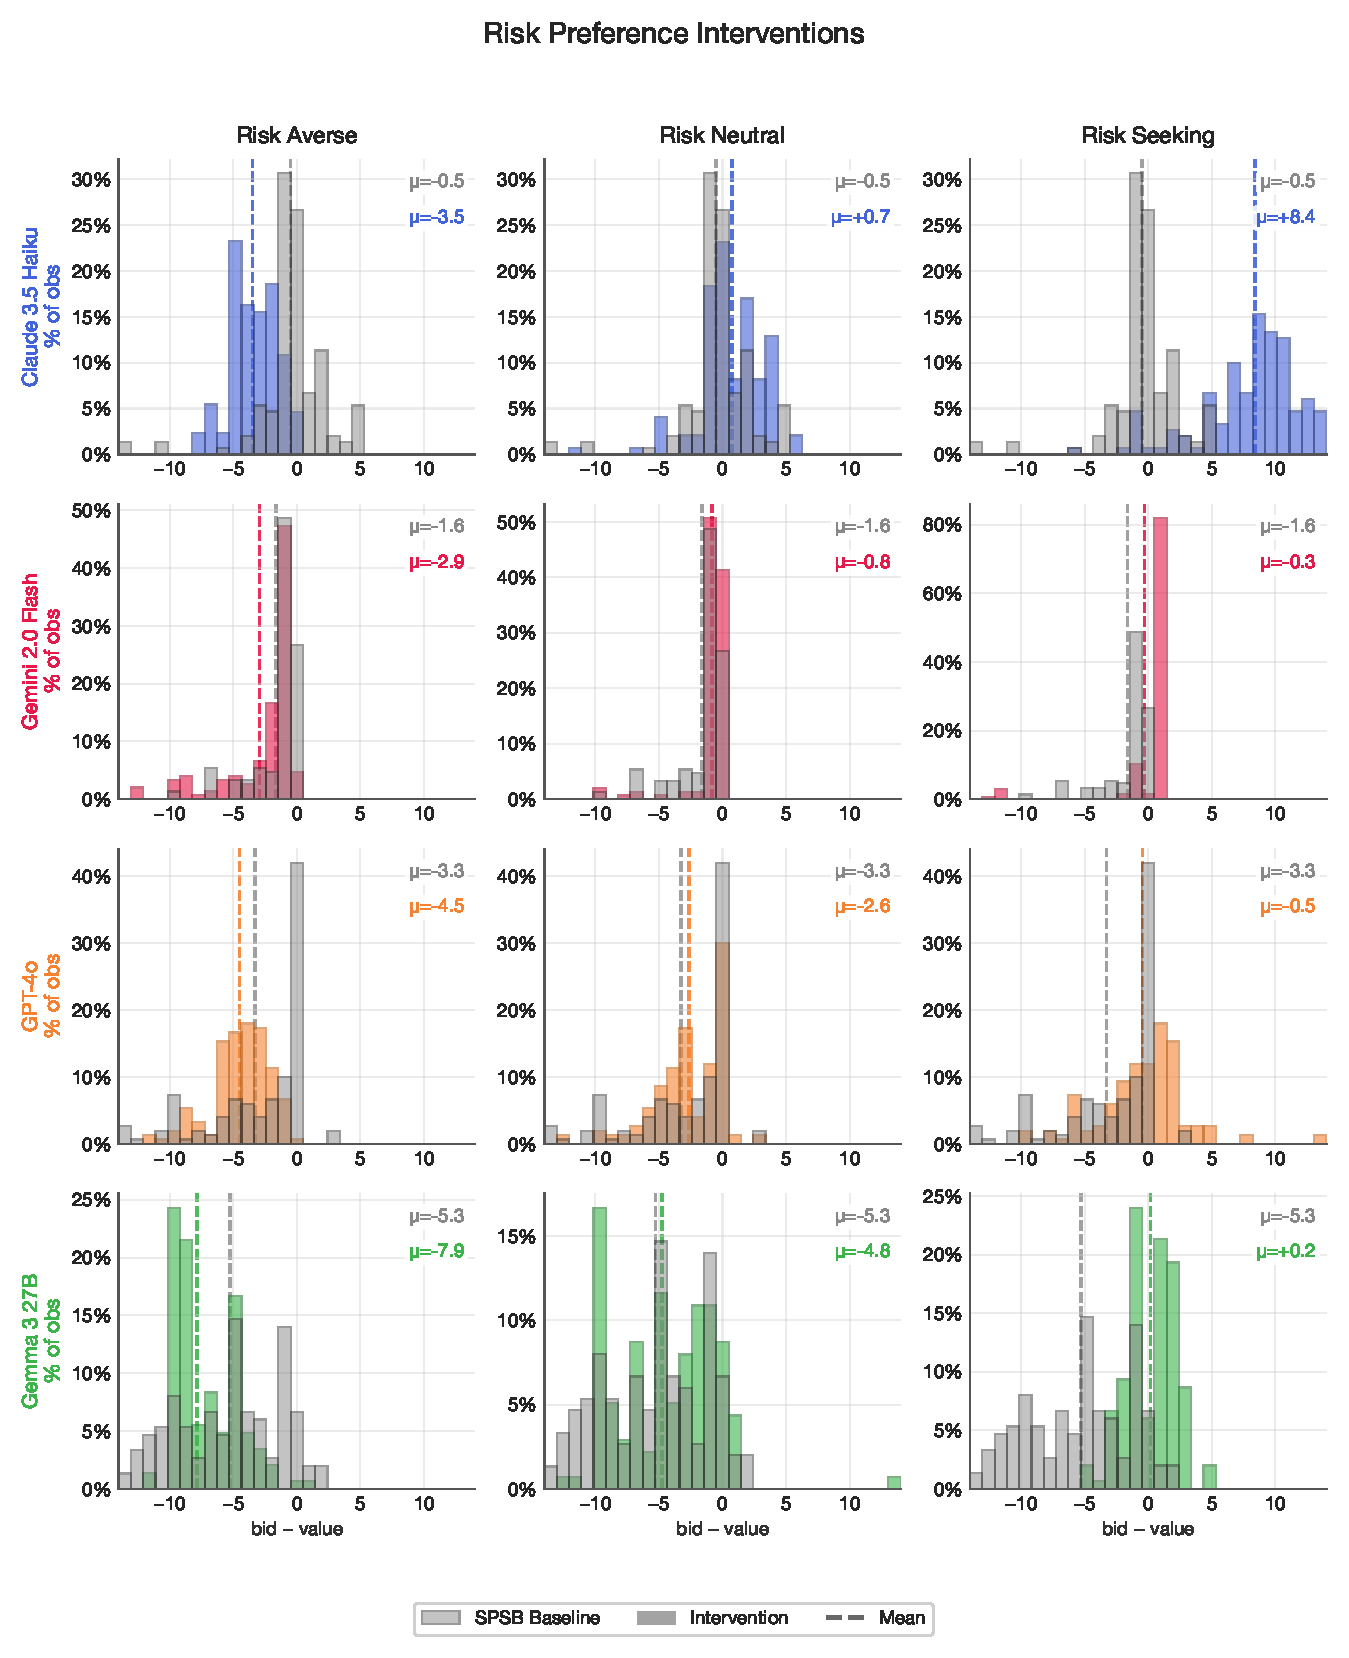
\includegraphics[width=\textwidth,height=0.85\textheight,keepaspectratio]{appendix_risk_preferences_auctions.pdf}
    \caption{Risk-preference personas in SPSB auctions (mean bid deviation from value, \$). Risk aversion increases underbidding ($\mu = -4.71$), while risk-seeking dramatically shifts Claude 3.5 Haiku to overbidding ($\mu = +8.40$). Risk neutrality ($\mu = -1.82$) modestly improves play relative to the SPSB baseline ($\mu = -2.67$).}
    \label{fig:prospect-risk-auctions}
\end{figure}

\begin{figure}[H]
    \centering
    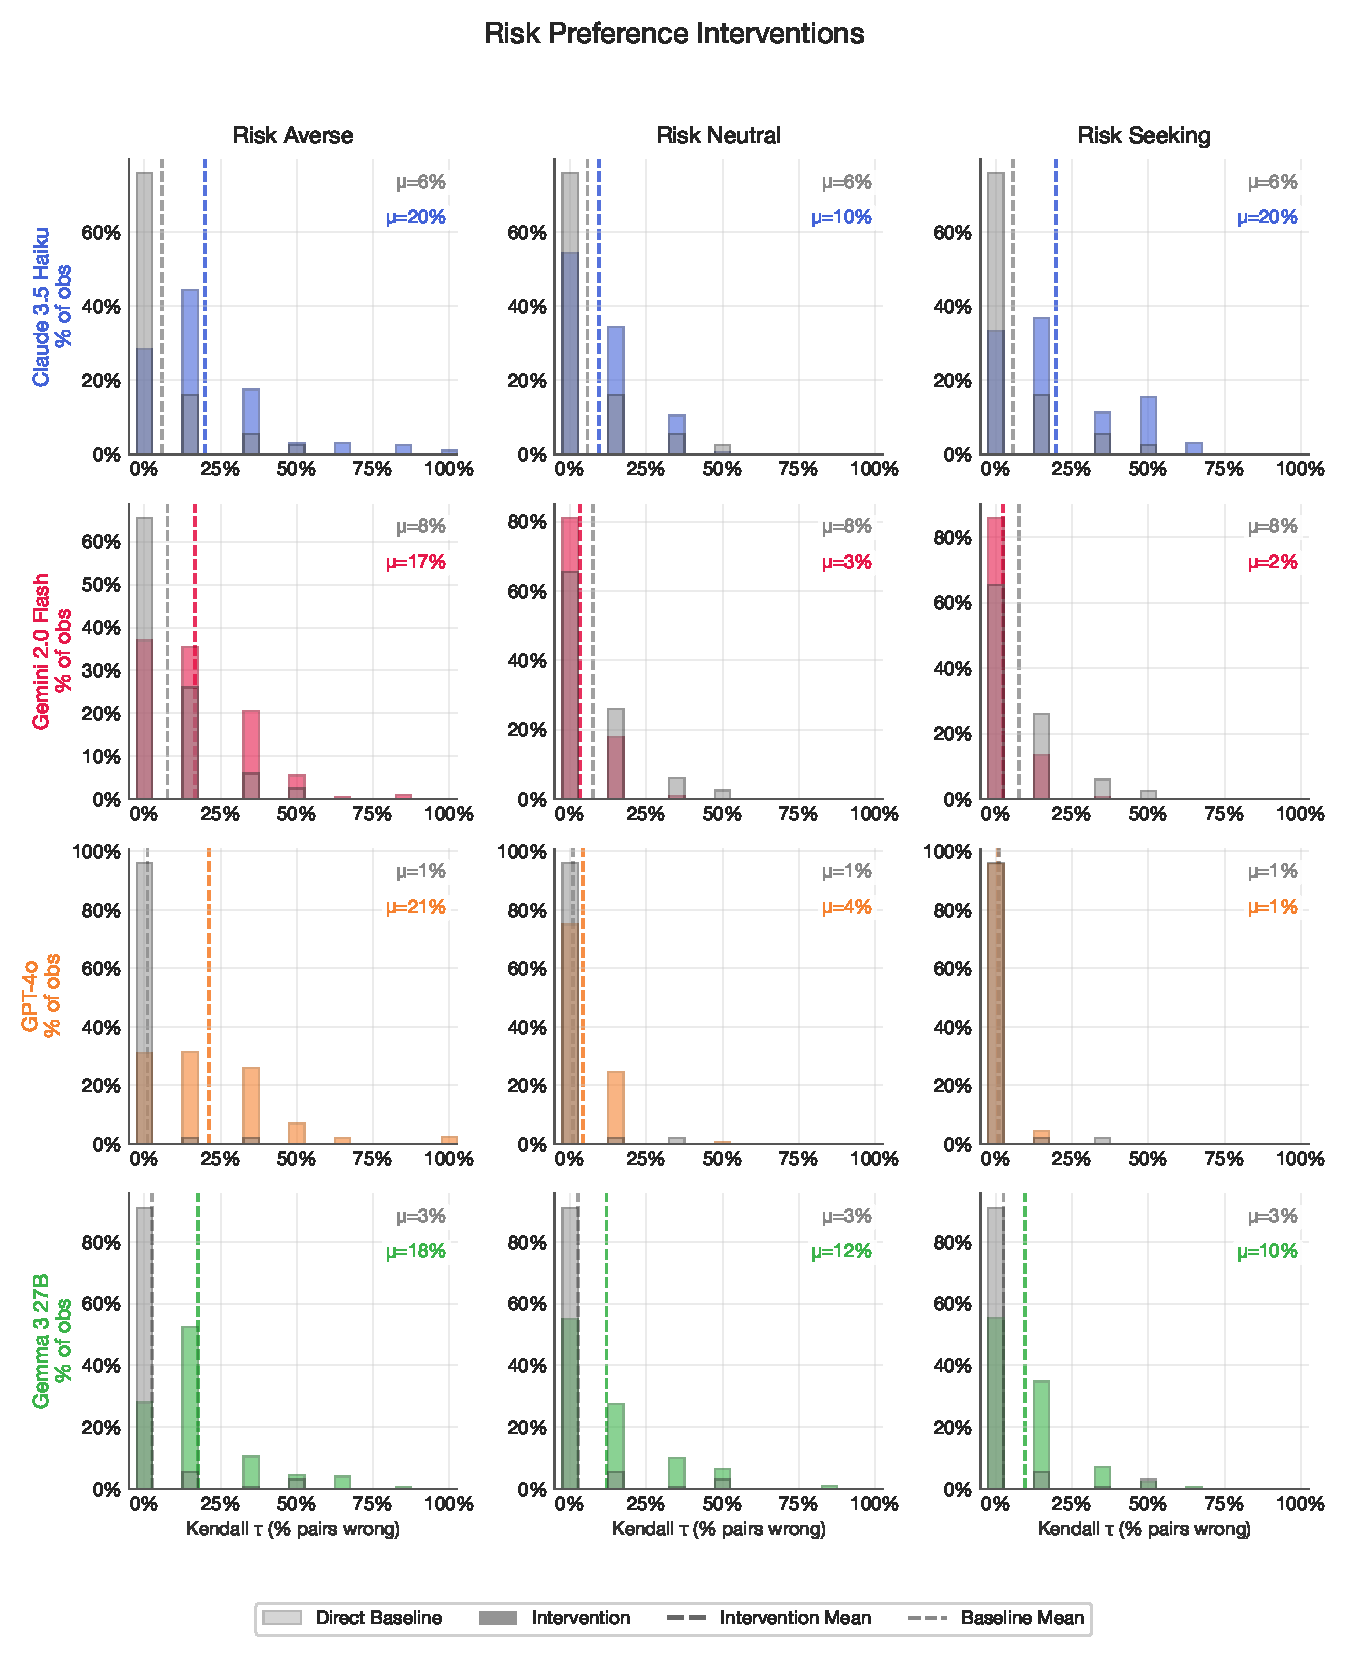
\includegraphics[width=\textwidth,height=0.85\textheight,keepaspectratio]{appendix_risk_preferences_da.pdf}
    \caption{Risk-preference personas in deferred acceptance (mean normalized Kendall-$\tau$ error, \%). Risk aversion dramatically worsens play ($\mu \approx 18.8\%$, compared to baseline $4.2\%$). Risk neutrality and risk-seeking also worsen play, though less severely.}
    \label{fig:prospect-risk-da}
\end{figure}

The risk interventions reveal that LLMs are highly responsive to persona-based instructions about risk attitudes, but that this responsiveness does not improve play. The risk-averse persona produces the most dramatic deterioration: in auctions, it increases underbidding from $\mu = -2.67$ to $-4.71$;\footnote{The per-model risk-averse cells reproduce from the imported pipeline (\texttt{writeup/auction-v2-numbers.txt}): Claude $-3.49$, Gemini $-2.94$, GPT-4o $-4.49$, Gemma $-7.86$, pooling to $-4.69$, which matches the $-4.71$ shown in Figure~\ref{fig:prospect-risk-auctions} up to rounding and cell-completion differences. \TODO{Finalize on the harmonized re-run (plan E3/E8); note the per-axis baseline-pooling caveat flagged in Section~\ref{sec:ranking}.}} in DA, it roughly quadruples the error rate ($\mu \approx 18.8\%$ against the $4.2\%$ baseline)---these two cells are the source of the bottom-rung $\rho$ values quoted above. The risk-seeking persona shifts Claude 3.5 Haiku to massive overbidding ($\mu = +8.40$), while the other models are less affected. Risk neutrality modestly improves auction play ($\mu = -1.82$) but worsens DA play. In aggregate, the models---while strategizing---are extremely susceptible to risk-preference priming.

These results underscore that the LLMs' failures in strategy-proof mechanisms are not driven by implicit risk attitudes. Truthful play is dominant regardless of risk preferences in both environments, so the fact that risk-persona instructions change behavior at all confirms that the models do not understand the mechanism's incentive structure. The risk interventions change \emph{how} models deviate from truth-telling, but do not address \emph{why} they deviate in the first place. For the ranking, the practical reading is a warning: persona-style ``preference'' instructions---a common ingredient in deployed agent stacks---are not neutral wrappers, and the risk-averse persona in particular is the most reliably harmful lever in our entire battery.

% ---------------------------------------------------------------------------
% Appendix: Prompt Library and Intervention Inventory
% Sources: Engineering_simplicity/contents/appendix.tex (prompt sections +
%   tab:all-interventions), writeup/contents/appendix.tex:577-605 (menu +
%   clock-framing prompts), verified against the repo templates in
%   Engineering_simplicity/engineer_simplicity-main/rule_template/{auctions,DA}/
%   and rule_template/V10,V12/ (old labels), and against the pipeline logs in
%   engineer_simplicity-main/experiment_logs/ (run-status audit).
% Implements plan §7.8 (no phantom results) and plan §5.6/§5.7 (old->new
%   taxonomy mapping; intervention_proxy_breitmoser split).
% Prompt texts are quoted verbatim from the templates actually sent to the
%   models (including their typos); non-ASCII glyphs are transliterated.
% ---------------------------------------------------------------------------
\section{Prompt Library and Intervention Inventory}\label{app:prompts}

This appendix documents the prompt templates behind every design lever used in the paper, organized by the taxonomy of Section~\ref{sec:framework}: Family~A (extensive-form implementations), Family~B (mechanism descriptions: B1 menu restatement, B2 safety-exposing, B3 clock-framing), Family~C (reasoning scaffolds: C1 contingent, C2 forward planning, C3 beliefs), and Family~D (preference framings, Appendix~\ref{app:prospect}). We present the full base-rule prompts for both domains; for each intervention we show only the text that is \emph{added to or modified from} the corresponding base prompt, since the surrounding context (bidder identity and response format in auctions; preference ordering, priorities, popularity signal, and output format in DA) remains identical. Template variables (e.g., \texttt{\{\{student\_id\}\}}, \texttt{\{\{preference\_order\}\}}, \texttt{\{\{increment\}\}}) are populated at runtime. The simulation pipeline that embeds these prompts is described in Appendix~\ref{app:procedures}; the DA protocol details are in Appendix~\ref{app:da}. Section~\ref{app:prompts-inventory} closes with the complete inventory (Table~\ref{tab:intervention-inventory}), which maps every repo-level template name to its final taxonomy family and records whether its results appear in this paper.

\subsection{Base rules}\label{app:prompts-base}

\paragraph{SPSB auction (IPV baseline).} The canonical baseline for the auction ranking cells (repo template \path{private_second_price}):

\begin{figure}[H]
\begin{lstlisting}
In this game, you will participate in an auction for a prize
against {{num_bidders}} other bidders. You will play this game
for {{n}} rounds.
At the start of each round, bidders will see their value for
the prize, randomly drawn between $0 and ${{private}}, with
all values equally likely.
After learning your value, you will submit a bid privately at
the same time as the other bidders. Bids must be in
${{increment}} increments.
The highest bidder wins the prize and pays the second-highest
bid. If you win, your earnings will increase by your value for
the prize, and decrease by the second-highest bid. If you don't
win, your earnings will remain unchanged.
After each auction, we will display all bids. Ties for the
highest bid will be resolved randomly.
\end{lstlisting}
\caption{SPSB auction, base rule (\texttt{private\_second\_price}). Standard second-price sealed-bid auction with independent private values. The FPSB, TPSB, APV, CV, and eBay rule prompts used in the validation exhibits (Section~\ref{sec:validation}) differ only in the allocation/payment paragraph and the value-model paragraphs; the eBay treatment prompts are summarized in Appendix~\ref{app:ebay}.}
\label{fig:prompt-spsb-base}
\end{figure}

\paragraph{Direct DA (traditional description).} The canonical DA baseline (\texttt{da\_direct\_traditional}) describes the full five-step student-proposing algorithm:

\begin{figure}[H]
\begin{lstlisting}
You are Student {{student_id}}. There are 4 schools: w, x, y, z.
You will be matched to at most one school.

HOW THE MATCHING WORKS (Deferred Acceptance):
1. All students simultaneously submit a ranking of schools
2. Each student "proposes" to their top-ranked school
3. Each school tentatively accepts the proposer it ranks highest
   (by priority), rejecting others
4. Rejected students propose to their next choice
5. This repeats until all students are matched

Your preference ordering (most preferred to least preferred):
  {{preference_order}}

Your priority rank at each school (1 = highest priority):
  w: {{pw}}, x: {{px}}, y: {{py}}, z: {{pz}}

Moreover, most applicants seem to favor {{global_ranking}}.

Submit a complete ranking of schools from most preferred to
least preferred.
Format: Ranking: <1st> > <2nd> > <3rd> > <4th>
\end{lstlisting}
\caption{Direct DA, base rule (\texttt{da\_direct\_traditional}). A \emph{null} variant (\texttt{da\_direct\_null}) is identical except that the ``HOW THE MATCHING WORKS'' block is removed entirely, providing no mechanism explanation; its results appear in Appendix~\ref{app:da} (Table~\ref{tab:intervention-inventory-da}).}
\label{fig:prompt-da-traditional}
\end{figure}

\subsection{Family A: extensive-form implementations}\label{app:prompts-osp}

\paragraph{Ascending clock (AC-B), per-tick query.} In the true iterative clock (final ID \path{osp_clock_iterative}), each auction consists of multiple clock cycles; at each posted price every remaining bidder is queried, and no dropout information is displayed, as in \citet{breitmoser2022obviousness}:

\begin{figure}[H]
\begin{lstlisting}
Your value towards to the prize is {value} in this round.
The current price in this clock cycle is {current_price}.
The price for next clock cycle is {current_price + increment}.

Do you want to stay in the bidding?
If you choose yes, you can keep bidding for next clock. If you
choose No, you will exit and have no chance to re-enter the
bidding. Your response must use these EXACT tags below. You
must output the ACTION.
    <PLAN> [...limit 50 words...] </PLAN>
    <ACTION> Yes or No </ACTION>
\end{lstlisting}
\caption{Ascending clock (AC-B), per-tick stay/exit query (final ID \texttt{osp\_clock\_iterative}). The bidder is first shown the auction rules (value model plus clock payment rule); the query above is repeated at every clock tick. See Appendix~\ref{app:procedures} for the full clock simulation loop and the AC (open) variant. On the \texttt{intervention\_proxy\_breitmoser} name collision affecting this lever, see Section~\ref{app:prompts-inventory}.}
\label{fig:prompt-clock-iterative}
\end{figure}

\paragraph{Iterative DA, binary-offer query.} The primary prompt at the binary-offer nodes of the OSP decision tree of \citet{ashlagi2018stable}; it explicitly states the consequence of each answer, providing the ``obviousness witness'' of that construction:

\begin{figure}[H]
\begin{lstlisting}
You are Student {{student_id}}. We are running a step-by-step
matching procedure.

Current remaining schools: {{remaining_set}}

Your preference ordering (most preferred to least preferred):
  {{preference_order}}

Your priority rank at each school (1 = highest priority):
  w: {{pw}}, x: {{px}}, y: {{py}}, z: {{pz}}

Moreover, most applicants seem to favor {{global_ranking}}.

Question: Among the remaining schools ({{remaining_set}}), is
  {{candidate}} your most preferred?
- If you answer YES: you are immediately matched to
  {{candidate}} and leave the process.
- If you answer NO: {{candidate}} remains available to you.
  You continue in the process with all current remaining
  schools ({{fallback_set}}).

<REASON> ... </REASON>
<DECISION> Answer: YES / NO </DECISION>
\end{lstlisting}
\caption{Iterative DA, yes/no query with consequence explanation (\texttt{da\_osp\_yesno}). At serial-dictatorship nodes, a companion prompt (\texttt{da\_osp\_choice}) instead asks the student to name their single most preferred school among the currently available set (``Do not list a full ranking. Do not condition on hypothetical future steps.'').}
\label{fig:prompt-da-osp-yesno}
\end{figure}

\subsection{Family B: mechanism descriptions}\label{app:prompts-desc}

\paragraph{B1 --- Menu restatement (auction).} Based on \citet{gonczarowski2023strategyproofness}, this replaces the payment paragraph of the SPSB base rule with a menu description (\texttt{intervention\_menu}):

\begin{figure}[H]
\begin{lstlisting}
Your "price to win" the item will be set to the highest bid
placed by any other player. If your bid is higher than this
"price to win," then you will win the item and pay this price.
If you don't win, your earnings will remain unchanged.
\end{lstlisting}
\caption{Menu restatement for SPSB (\texttt{intervention\_menu}, Family B1). Reported in Section~\ref{sec:ranking-descriptions} for all four models: small, sign-mixed effects across models and null on average.}
\label{fig:prompt-menu}
\end{figure}

\paragraph{B1 --- Menu restatement (DA).} Two DA analogues exist as templates, \path{da_direct_menu_property} and \path{da_direct_menu_mechanics}; both restate DA through the obtainable-schools menu, following \citet{gonczarowski2023strategyproofness}. Both are reported in Appendix~\ref{app:da}, where they split sharply by content. The \emph{property} variant reads:

\begin{figure}[H]
\begin{lstlisting}
KEY PROPERTY OF THIS MECHANISM:
Given the other students' rankings and school priorities, there
is a fixed set of schools you could possibly be matched with
(your "Obtainable Schools").

IMPORTANT: Your ranking CANNOT change what is in your Obtainable
Schools. Your ranking ONLY determines which school you receive
WITHIN that set - you get your highest-ranked school among the
obtainable ones.
\end{lstlisting}
\caption{Menu restatement for DA, property variant (\texttt{da\_direct\_menu\_property}, Family B1). The \emph{mechanics} variant states the same construction procedurally (``Step 1: \ldots the mechanism computes your Obtainable Schools. Step 2: You receive the school you ranked highest among your Obtainable Schools.'') \emph{without} the invariance statement. Both are reported in Appendix~\ref{app:da}: the property variant significantly improves truthful reporting (pooled $4.2\% \to 1.8\%$), the mechanics variant significantly worsens it ($4.2\% \to 6.9\%$).}
\label{fig:prompt-da-menu}
\end{figure}

\paragraph{B2 --- Payoff Safety (auction).} Surfaces the pivotality property behind \citet{vickrey1961counterspeculation}'s strategy-proofness argument (old labels \path{axis2_forward_onestep} / \path{axis1_contingent_onestep}; final ID \emph{Payoff Safety}):

\begin{figure}[H]
\begin{lstlisting}
**How the auction works:**
Think of your bid as setting your "maximum price." The auction
will find the highest price below your maximum that still wins.
Specifically:
- If your bid is the highest, you win and pay the second-highest
  bid
- If your bid is not the highest, you don't win and pay nothing

This means: Your bid only matters for determining IF you win,
not HOW MUCH you pay. You can think of it simply as: "At what
price would I no longer want the item?"
\end{lstlisting}
\caption{Payoff Safety description for SPSB (Family B2). Despite the ``axis-2 / forward-planning'' repo filename, this is a mechanism description, not a reasoning scaffold: it states \emph{what is true} of the payment rule rather than instructing a mode of reasoning (see the mapping notes in Section~\ref{app:prompts-inventory}).}
\label{fig:prompt-payoff-safety}
\end{figure}

\paragraph{B2 --- Rejection Safety (DA).} Surfaces the property that distinguishes DA from the Boston mechanism \citep{abdulkadirouglu2003school}: rejections are safe (old label \path{axis2_da_monotonic_safety}; final ID \emph{Rejection Safety}):

\begin{figure}[H]
\begin{lstlisting}
KEY INSIGHT - REJECTIONS ONLY REDIRECT, NEVER ELIMINATE:
In this matching process:
- Being rejected from a school you ranked highly does NOT hurt
  your chances at schools ranked lower
- You cannot be "knocked out" of a school that would have
  accepted you
- The algorithm protects you: rejections only happen BEFORE you
  would have been matched

Your ranking determines the ORDER in which you're considered,
not WHETHER you're considered.
\end{lstlisting}
\caption{Rejection Safety description for DA (Family B2). Two sibling ``monotonicity'' templates (\texttt{axis2\_da\_monotonic\_options}: ``your options never shrink''; \texttt{axis2\_da\_monotonic\_outcome}: ``the obtainable set determines the outcome'') were run but are not reported (Table~\ref{tab:intervention-inventory}).}
\label{fig:prompt-rejection-safety}
\end{figure}

\paragraph{B3 --- Clock-framing (auction).} Based on \citet{breitmoser2022obviousness}, this \emph{describes} the sealed bid as an automatic exit threshold in a simulated clock---a description change only; the game remains a one-shot sealed-bid auction (repo template \path{intervention_proxy_breitmoser}; final ID \path{desc_clock_framing}):

\begin{figure}[H]
\begin{lstlisting}
**FIRST STAGE: Sealed Bid**
You will submit a sealed bid privately at the same time as the
other bidders. This bid will serve as your automatic exit price
in the next stage.
**SECOND STAGE: Ascending Clock (Simulation)**
After the sealed bid stage, we will simulate an ascending clock
auction. The clock will start at $0 and increase in increments
of ${{increment}}. The clock will display the current price.
You will also see that there are a total of {{num_bidders}}
bidders participating, although you do not know other bidder's
values. If the current price on the clock reaches or exceeds
your sealed bid from the first stage, you will automatically
exit the auction. The auction ends when only one bidder is left
remaining in the second stage based on their bid from the first
stage.
**END OF AUCTION**
If you win, your earnings will increase by your value for the
prize and decrease by the clock price at the end of the auction.
If you don't win, your earnings will remain unchanged.
\end{lstlisting}
\caption{Clock-framing description for SPSB (Family B3; final ID \texttt{desc\_clock\_framing}). The elicited action is still a single sealed bid; no per-tick queries occur. Never to be conflated with the true iterative clock of Figure~\ref{fig:prompt-clock-iterative}; see the name-collision note in Section~\ref{app:prompts-inventory}.}
\label{fig:prompt-clock-framing}
\end{figure}

\subsection{Family C: reasoning scaffolds}\label{app:prompts-scaffold}

\paragraph{C1 --- Payoff Tree (auction).} Presents the explicit decision tree of outcomes (old labels \path{axis2_forward_tree} and \path{axis1_contingent_tree}; final ID \emph{Payoff Tree}; classified C1 contingent reasoning---see Section~\ref{app:prompts-inventory}):

\begin{figure}[H]
\begin{lstlisting}
**Decision Tree:**
Consider your decision as follows:

You choose bid B. Then one of two things happens:

  PATH A: Your bid B > all other bids
    -> You WIN
    -> You pay: second-highest bid (call it P)
    -> Your profit: (Your Value) - P
    -> Note: P < B, so if Value >= B, then profit >= 0

  PATH B: Your bid B <= some other bid
    -> You LOSE
    -> You pay: $0
    -> Your profit: $0

Key insight: In PATH A, you pay P (not B). So bidding higher
than your value only matters if it changes whether you're in
PATH A vs PATH B.
\end{lstlisting}
\caption{Payoff Tree scaffold for SPSB (Family C1). Non-ASCII arrows in the repo template are transliterated as \texttt{->}.}
\label{fig:prompt-tree-auction}
\end{figure}

\paragraph{C1 --- Payoff Tree (DA).} The DA analogue (\texttt{axis1\_da\_tree}) replaces the algorithm description with a tree view:

\begin{figure}[H]
\begin{lstlisting}
HOW THE MATCHING WORKS (Decision Tree View):
Think of DA as a tree of possibilities:
- ROOT: You propose to your 1st choice
  - If ACCEPTED: You're matched to that school
  - If REJECTED: You propose to your 2nd choice
    - If ACCEPTED: You're matched to that school
    - If REJECTED: You propose to your 3rd choice
      - And so on...

At each branch, acceptance/rejection depends on the school's
priorities and who else proposed there.
\end{lstlisting}
\caption{Payoff Tree scaffold for DA (Family C1). Additional C1 variants in both domains (\emph{Enumerate}, \emph{Dominated}, \emph{Worst-Case}, \emph{Backward-Induction} framings) were run but are not reported; see Table~\ref{tab:intervention-inventory}. The \emph{Enumerate} variant, for example, asks: ``What are the possible bids the other players might submit? For each possible bid they might make, what would be your best response?'' (auctions), or the analogous question over rankings (DA).}
\label{fig:prompt-tree-da}
\end{figure}

\paragraph{C2 --- Forward-planning lookahead (DA only).} Scaffolds $k$-step simulation of the DA algorithm's internal rounds \citep{pycia2023theory}; SPSB has no analogous internal dynamics, so C2 is DA-only (Section~\ref{sec:framework}). The $k{=}1$ variant (\texttt{axis2\_da\_1step}):

\begin{figure}[H]
\begin{lstlisting}
HOW THE MATCHING WORKS:
You submit a ranking. The algorithm processes your ranking
sequentially:
- First, you "propose" to your top-ranked school
- If accepted, you're matched there
- If rejected, you propose to your second choice

THINK ONE STEP AHEAD:
Before finalizing your ranking, consider: If you are rejected
from your first choice, which school would you propose to next?
Does this affect how you should rank schools?
\end{lstlisting}
\caption{One-step lookahead scaffold for DA (Family C2, \texttt{axis2\_da\_1step}). The $k{=}2$ variant (\texttt{axis2\_da\_2step}) extends the framing to the first two potential rejections (``Plan your ranking with these two steps in mind''). The $k{=}0$ and $k{=}\infty$ (full-simulation) variants were run but are not reported.}
\label{fig:prompt-lookahead}
\end{figure}

\paragraph{C3 --- Belief scaffolds (both domains).} First- and second-order belief prompts appended to the base rules. In auctions (\texttt{axis3\_beliefs\_firstorder}, \texttt{axis3\_beliefs\_secondorder}):

\begin{figure}[H]
\begin{lstlisting}
[First-order]
The other bidders are rational agents who are also trying to
maximize their earnings.
Before bidding, ask yourself: What do I expect the other bidders
to bid? Given their values are also drawn randomly between $0
and ${{private}}, and they want to maximize their earnings, how
do I think they will behave? Does this affect what I should bid?

[Second-order]
Before bidding, consider the following: What do the other
bidders think YOU will bid? They know you are rational and
trying to maximize your earnings. They might try to anticipate
your strategy. Does their belief about your behavior affect what
they will do? And does that, in turn, affect what you should do?
\end{lstlisting}
\caption{Belief scaffolds for SPSB (Family C3). The DA analogues (\texttt{axis3\_da\_firstorder}, \texttt{axis3\_da\_secondorder}) ask ``What rankings do you think the other students will submit?'' and ``What do you think the other students believe YOU will rank?'' respectively. A \emph{Common Knowledge} variant in each domain (emphasizing common knowledge of rationality) was run but is not reported.}
\label{fig:prompt-beliefs}
\end{figure}

\subsection{Family D: preference framings}\label{app:prompts-prospect}

The Family-D battery (results in Appendix~\ref{app:prospect}) replaces or augments the objective framing rather than the mechanism explanation. As one representative, the risk-averse persona (\path{intervention_risk_averse}, identical wording in both domains modulo context):

\begin{figure}[H]
\begin{lstlisting}
You are risk-averse. This means that you are the type of person
that would only pay $4 for a coin toss where you got $0.00 on
tails and $10.00 on heads (even though the expected value is
$5.00). You prefer to avoid uncertainty and would rather have a
guaranteed outcome than take a risky gamble, even if the gamble
has the same or slightly higher expected value.
\end{lstlisting}
\caption{Risk-averse persona (Family D). Risk-neutral and risk-seeking personas change only the coin-toss price (\$5, \$6); the loss-aversion battery (gain/loss/mixed frames, endowment, WTA/WTP) is described in Appendix~\ref{app:prospect-loss}.}
\label{fig:prompt-risk-persona}
\end{figure}

\subsection{Intervention inventory and old-to-new mapping}\label{app:prompts-inventory}

The prompt templates accumulated across two experimental programs and several repo versions, and three of the resulting labels are actively misleading. We fix the mapping here once, and Table~\ref{tab:intervention-inventory} applies it to every template in the repo.

\paragraph{Taxonomy corrections (plan reconciliation R7).} (i)~\emph{Payoff Tree} carries the repo filename \path{axis2_forward_tree.txt} (V12) / \path{axis1_contingent_tree.txt} (imported pipeline), but SPSB is a one-shot game with no own future decision points, so there is no forward-planning axis to scaffold; the intervention lays out payoff-relevant \emph{contingencies} and is classified C1. (ii)~\emph{Payoff Safety} (\path{axis2_forward_onestep} / \path{axis1_contingent_onestep}) and \emph{Rejection Safety} (\path{axis2_da_monotonic_safety}) state true properties of the payment/rejection rule without instructing any mode of reasoning; both are descriptions (B2), not scaffolds. (iii)~Clock-framing is a description (B3), not an extensive-form change.

\paragraph{The \texttt{intervention\_proxy\_breitmoser} name collision (plan reconciliation R6).} The single template name \path{intervention_proxy_breitmoser} has been used for two different objects: (a)~in the ES appendix, it labels the \emph{true iterative clock} prompt (per-tick stay/exit queries, Figure~\ref{fig:prompt-clock-iterative}); (b)~in the repo template files (\path{rule_template/V10/}, \path{V12/}, and the imported pipeline's \path{rule_template/auctions/}), it is the \emph{two-stage sealed-bid clock-framing description} (Figure~\ref{fig:prompt-clock-framing}). We split the ID: \path{osp_clock_iterative} (Family A) vs.\ \path{desc_clock_framing} (Family B3). Our audit of the imported pipeline supports the split as follows: the logs stored under \path{experiment_logs/<model>/intervention_proxy_breitmoser/} record exactly one sealed bid per bidder per auction (no tick-by-tick decisions), i.e., they are \path{desc_clock_framing} runs; whereas the clock column of the OSP comparison (Figure~\ref{fig:osp-comparison}) reproduces numerically from the pipeline's \path{ascending_clock_closed} cells, which are true per-tick clock runs (in the APV environment---see the provenance flag in Section~\ref{sec:ranking-extensive}). The audit is settled: the pipeline template behind \path{intervention_proxy_breitmoser} is the \emph{description} variant (\path{desc_clock_framing}), and the OSP clock column is computed from the \path{ascending_clock_closed} cells. With both IDs now reported for all four models (Sections~\ref{sec:ranking-extensive} and~\ref{sec:ranking-descriptions}), ranking rungs A (true clock) and B3 (clock-framing) are empirically distinguished model by model.

\paragraph{Run-status audit.} Table~\ref{tab:intervention-inventory} records, for every declared template, whether its results are reported in this paper (with the section), were \emph{run but not reported} (logs exist in \path{engineer_simplicity-main/experiment_logs/} or in the git-recovered writeup logs, but the cells do not appear in any exhibit), or were \emph{not run} on the canonical grid. This implements the no-phantom-results rule (plan \S7.8): no template is silently declared.

\paragraph{Comparison-baseline declaration.} Two families of sealed-bid SPSB baselines coexist in the pipeline, and the paper uses them for different purposes: OSP and extensive-form comparisons quote the \emph{dedicated} \texttt{spsb} cells (mean deviations $-0.49$/$-1.63$/$-3.28$/$-5.27$ for Claude/Gemini/GPT-4o/Gemma, matching the previously published $-0.5$/$-1.6$/$-3.3$/$-5.3$), while intervention contrasts use the \emph{axis-specific} baselines (each \texttt{axisK\_*} treatment against its same-axis baseline; the pooled axis baseline for the \texttt{intervention\_*} cells). Both baseline sets, and every treatment cell, are recorded with bootstrap confidence intervals in \path{results/merged_ranking/auction_cells.csv}.

\begin{table}[p]
\centering
\footnotesize
\setlength{\tabcolsep}{4pt}
\begin{tabular}{p{4.9cm} p{3.3cm} p{1.0cm} p{4.4cm}}
\toprule
\textbf{Old label (repo template)} & \textbf{Final taxonomy family} & \textbf{Domain} & \textbf{Reported in paper?} \\
\midrule
\multicolumn{4}{l}{\emph{Panel A: Auctions}} \\
\midrule
\texttt{private\_second\_price} & Baseline (SPSB, IPV) & Auction & Yes (\S\ref{sec:validation}, \S\ref{sec:ranking}) \\
\texttt{affiliated\_spsb}; \texttt{affiliated\_ac}; \texttt{affiliated\_ac\_closed} & Baseline (APV); A (AC); A (AC-B) & Auction & Yes (\S\ref{sec:validation}, \S\ref{sec:ranking-extensive}) \\
\texttt{intervention\_proxy\_breitmoser} (ES-appendix usage) $\to$ \texttt{osp\_clock\_iterative} & A (extensive form) & Auction & Yes (\S\ref{sec:ranking-extensive}); clock column = \texttt{ascending\_clock\_closed} cells (provenance settled; see below) \\
\texttt{intervention\_proxy\_breitmoser} (repo template) $\to$ \texttt{desc\_clock\_framing} & B3 (clock-framing) & Auction & Yes, all four models (\S\ref{sec:ranking-descriptions}); large improvement in every model ($p<0.001$) \\
\texttt{intervention\_menu} & B1 (menu restatement) & Auction & Yes, all four models (\S\ref{sec:ranking-descriptions}); sign-mixed, null on average \\
\texttt{axis2\_forward\_onestep} = \texttt{axis1\_contingent\_onestep} $\to$ Payoff Safety & B2 (safety-exposing) & Auction & Yes (\S\ref{sec:ranking-descriptions}) \\
\texttt{axis2\_forward\_tree} = \texttt{axis1\_contingent\_tree} $\to$ Payoff Tree & C1 (contingent) & Auction & Yes (\S\ref{sec:ranking-scaffolds}) \\
\texttt{axis1\_contingent\_\{enumerate, dominated, worstcase\}} & C1 (contingent) & Auction & Run; the \emph{Worst-Case} cell enters the trace analysis as a manipulation check (App.~\ref{app:traces}); \emph{Enumerate}/\emph{Dominated} not reported \\
\texttt{axis2\_forward\_backward\_induct} = \texttt{axis1\_contingent\_backward\_induct} & C1 (two-stage framing) & Auction & Run, not reported \\
\texttt{axis3\_beliefs\_firstorder}; \texttt{axis3\_beliefs\_secondorder} & C3 (beliefs) & Auction & Yes (\S\ref{sec:ranking-scaffolds}) \\
\texttt{axis3\_beliefs\_common\_knowledge} & C3 (beliefs) & Auction & Run, not reported \\
\texttt{axis1\_contingent\_baseline}; \texttt{axis2\_forward\_baseline}; \texttt{axis3\_beliefs\_baseline}; \texttt{loss\_aversion\_baseline} & Per-axis baselines & Auction & Yes, as comparison baselines for axis-matched treatment cells (see the comparison-baseline declaration above) \\
\texttt{intervention\_risk\_\{averse, neutral, seeking\}} & D (risk personas) & Auction & Yes (App.~\ref{app:prospect}) \\
\texttt{loss\_aversion\_\{gain\_frame, loss\_frame, mixed\_frame, endowment, WTA\_WTP\}} & D (loss/endowment frames) & Auction & Yes (App.~\ref{app:prospect}) \\
\texttt{intervention\_NE\_strat\_reveal}; \texttt{intervention\_wrong\_strat\_reveal}; \texttt{intervention\_nash\_deviation} & Excluded: advice (reveals or misstates the strategy; not a simplicity-preserving lever) & Auction & Run, not reported \\
\texttt{first\_price\_interventions/*}; \texttt{third\_price\_interventions/*} & Out of ranking scope (BNE benchmark, not dominant-strategy) & Auction & Partially run, not reported; parked per plan \S6 scope decision \\
\texttt{robust\_*} (currency/language); \texttt{private\_all\_pay*} & Legacy V10 robustness & Auction & Run in earlier drafts, not reported (cut, plan \S7.9) \\
\bottomrule
\end{tabular}
\caption{Intervention inventory (Panel A: auctions): every declared prompt template, its final taxonomy family (Section~\ref{sec:framework}), and its run/reporting status. ``Run, not reported'' means raw logs exist in the imported pipeline (\texttt{Engineering\_simplicity/engineer\_simplicity-main/experiment\_logs/}) or the git-recovered writeup logs, but the cell appears in no exhibit of this paper. Old labels are repo filenames; where the V12 writeup name and the imported-pipeline name differ, both are given with ``=''. Panel B (deferred acceptance) continues in Table~\ref{tab:intervention-inventory-da}.}
\label{tab:intervention-inventory}
\end{table}

\begin{table}[p]
\centering
\footnotesize
\setlength{\tabcolsep}{4pt}
\begin{tabular}{p{4.9cm} p{3.3cm} p{1.0cm} p{4.4cm}}
\toprule
\textbf{Old label (repo template)} & \textbf{Final taxonomy family} & \textbf{Domain} & \textbf{Reported in paper?} \\
\midrule
\multicolumn{4}{l}{\emph{Panel B: Deferred acceptance}} \\
\midrule
\texttt{da\_direct\_traditional} & Baseline (direct DA) & DA & Yes (App.~\ref{app:da}) \\
\texttt{da\_direct\_null} & Baseline variant (no explanation) & DA & Yes (App.~\ref{app:da}); heterogeneous across models \\
\texttt{da\_direct\_textbook\_sp} & Direct SP statement (reveals the dominant strategy) & DA & Yes, as a diagnostic ceiling (App.~\ref{app:da}): $0.0\%$ error for all four models; excluded from the lever ranking \\
\texttt{da\_direct\_menu\_property}; \texttt{da\_direct\_menu\_mechanics} & B1 (menu restatement) & DA & Yes (App.~\ref{app:da}); property variant improves play, mechanics variant backfires \\
\texttt{da\_osp\_yesno} (+ \texttt{da\_osp\_choice} node prompt; \texttt{da\_osp\_yesno\_guaranteed}) & A (iterative DA) & DA & Yes (App.~\ref{app:da}); the pick-based protocol is the canonical iterative-DA cell, the yes/no tree appears in the decision-level accounting \\
\texttt{axis1\_da\_tree} $\to$ Payoff Tree (DA) & C1 (contingent) & DA & Yes (App.~\ref{app:da}) \\
\texttt{axis1\_da\_\{enumerate, dominated, worstcase, onestep, backward\_induct\}} & C1 (contingent) & DA & Run, not reported \\
\texttt{axis2\_da\_1step}; \texttt{axis2\_da\_2step} & C2 (forward planning) & DA & Yes (App.~\ref{app:da}) \\
\texttt{axis2\_da\_0step}; \texttt{axis2\_da\_fullsim} & C2 (forward planning) & DA & Run, not reported \\
\texttt{axis2\_da\_monotonic\_safety} $\to$ Rejection Safety & B2 (safety-exposing) & DA & Yes (App.~\ref{app:da}) \\
\texttt{axis2\_da\_monotonic\_options}; \texttt{axis2\_da\_monotonic\_outcome} & B2 variants & DA & Run, not reported \\
\texttt{axis3\_da\_firstorder}; \texttt{axis3\_da\_secondorder} & C3 (beliefs) & DA & Yes (App.~\ref{app:da}) \\
\texttt{axis3\_da\_common\_knowledge} & C3 (beliefs) & DA & Run, not reported \\
\texttt{intervention\_risk\_\{averse, neutral, seeking\}} (DA) & D (risk personas) & DA & Yes (App.~\ref{app:prospect}) \\
\texttt{loss\_aversion\_*} (DA) & D (loss/endowment frames) & DA & Yes (App.~\ref{app:prospect}) \\
\texttt{da\_cardinal} variants (pipeline) & Environment variant (cardinal payoffs) & DA & Run, not reported \\
\bottomrule
\end{tabular}
\caption{Intervention inventory, continued (Panel B: deferred acceptance). Conventions as in Table~\ref{tab:intervention-inventory}. The eBay treatment prompts (T1--T4) belong to the eBay environment rather than the lever taxonomy and are catalogued in Appendix~\ref{app:ebay}.}
\label{tab:intervention-inventory-da}
\end{table}

% ---------------------------------------------------------------------------
% Appendix: Reasoning-trace analysis, details.
% Wired into the master after appendix_prompts (integrator pass 2026-07-07).
%
% Sources (all numbers): analysis/build_trace_features.py outputs in
%   results/traces/ — trace_features.csv (21,990 traces), ols_results.txt
%   (cluster-robust OLS + mediation + dedup robustness),
%   feature_prevalence_model_family.csv, feature_prevalence_mechanism_gpt4o.csv,
%   traces_summary.md, BRAINSTORM.md (further-directions options).
%   Bootstrap/OLS seed: numpy 1299.
% ---------------------------------------------------------------------------
\section{Reasoning-Trace Analysis: Details}\label{app:traces}

Every bid in our experiments is accompanied by a short free-text plan (median 68 words) in which the agent explains its choice. This appendix documents the measurement apparatus behind the trace results reported in the main text (Section~\ref{sec:ranking-traces}): the corpus, the keyword dictionary, full prevalence tables, the pooled regression with its honestly modest explanatory power, the mediation detail behind the double dissociation, and robustness to duplicate traces. Throughout, the plans are stated strategies, not full chains of thought; models may compute more (or less) than they verbalize, so every claim here concerns what models \emph{say}, validated against what they \emph{do}.

\subsection{Corpus and Feature Dictionary}\label{app:traces-dictionary}

The corpus contains 21{,}990 traces from three sources: (i)~13{,}416 traces from the harmonized four-model grid (92 run directories covering the sealed-bid SPSB baseline and intervention cells plus the closed clock); (ii)~1{,}167 traces from the menu-restatement (B1) and clock-framing (B3) cells, all four models; and (iii)~7{,}407 recovered GPT-4o traces from the FPSB (3{,}711) and TPSB (3{,}696) variants of the same grid, which provide the cross-mechanism contrast. Duplicate second-price cells present in both (i) and (iii) were excluded from (iii) to prevent double counting. Each trace row carries its run directory as a cluster identifier; all standard errors below are cluster-robust at the run level. Ascending-clock traces (510 rows) are per-decision exit rationales, structurally different from sealed-bid plans; they are retained in the corpus but excluded from the pooled regressions.

We score each trace with eighteen binary keyword features (Table~\ref{tab:trace-dictionary}), applied as transparent regular expressions (full patterns in \path{analysis/build_trace_features.py}). The features were tuned on the language models actually produce: an initial dictionary keyed to the theory's vocabulary (``no risk,'' ``can't lose'') turned out to be essentially absent from real traces---the \texttt{safety\_recognition} feature, which detects an echo of the Payoff Safety invariant, fires on 3 of 21{,}990 traces---so the safety/risk group was re-anchored on the words models use (``overpay,'' ``profit margin,'' ``buffer,'' ``zero profit''). The dictionary does no negation handling by design: \texttt{overpay\_concern} counts ``avoid overpaying'' as overpayment rhetoric either way, which is the intended reading.

\begin{table}[htbp]
\centering
\footnotesize
\setlength{\tabcolsep}{5pt}
\begin{tabular}{llp{8.2cm}}
\toprule
Group & Feature & Fires when the plan\ldots \\
\midrule
Normative & \texttt{dominance\_language} & invokes dominance (``dominant strategy,'' ``regardless of others'') \\
recognition & \texttt{truthful\_intent} & states an intent to bid exactly one's value \\
& \texttt{payment\_rule\_correct} & correctly rehearses that the winner pays the second-highest bid \\
& \texttt{second\_price\_mention} & name-drops ``second-highest''/``second price'' (weak rule mention) \\
& \texttt{first\_price\_mention} & calls the auction ``first-price'' (mechanism confusion) \\
\addlinespace
Opponents \& & \texttt{opponent\_modeling} & speculates about other bidders' values or bids \\
beliefs & \texttt{probability\_reasoning} & uses chance/likelihood language \\
& \texttt{expected\_value\_reasoning} & computes or invokes expected value \\
\addlinespace
Stated intent & \texttt{shading\_intent} & states an intent to bid \emph{below} value (value-anchored) \\
& \texttt{overbid\_intent} & states an intent to bid \emph{above} value (value-anchored) \\
\addlinespace
Safety / risk & \texttt{worst\_case} & reasons about the worst case \\
rhetoric & \texttt{safety\_recognition} & echoes the B2 invariant (``bid determines if you win, not what you pay'') \\
& \texttt{overpay\_concern} & worries about overpaying \\
& \texttt{zero\_profit\_fallacy} & argues that bidding one's value yields zero profit \\
& \texttt{margin\_language} & invokes a profit margin or buffer \\
\addlinespace
Style & \texttt{conservative\_language} & self-describes as cautious/conservative \\
& \texttt{aggressive\_language} & self-describes as aggressive/competitive \\
& \texttt{risk\_language} & uses risk vocabulary \\
\bottomrule
\end{tabular}
\caption{The trace feature dictionary: eighteen binary keyword features in five groups. Exact regular expressions and per-cell prevalence are in the replication package (\texttt{analysis/build\_trace\_features.py}; \texttt{results/traces/trace\_features.csv}).}
\label{tab:trace-dictionary}
\end{table}

\subsection{Prevalence: Model Fingerprints and Mechanism Insensitivity}\label{app:traces-prevalence}

Table~\ref{tab:trace-prevalence-models} reports feature prevalence in the baseline SPSB cells by model; Table~\ref{tab:trace-prevalence-mechanisms} reports prevalence by sealed-bid mechanism for GPT-4o. Pooling all 14{,}073 sealed second-price traces, the modal story a model tells itself is textbook \emph{first-price} logic applied to a second-price auction: 53\% state an intent to shade below value, 55\% worry about overpaying, and 31\% invoke a profit margin, while dominance language appears in 2.1\% of traces, correct payment-rule rehearsal in 3.8\%, and stated truthful intent in 6.8\%.

Each model has a recognizable fingerprint (pooled sealed second-price cells). Gemini is a near-pure shader (\texttt{shading\_intent} 86\%, \texttt{overbid\_intent} 4.5\%). Claude is the only model that explicitly mislabels the mechanism ``first-price'' (10.0\% of its traces versus at most 0.1\% elsewhere) and has both the most stated overbidding (30\%) and the most stated truthful intent (12.6\%)---the noisiest stated strategy. Gemma produces the least value-anchored language (\texttt{shading\_intent} 10.6\%) but the most opponent modeling (49\%), conservative self-description (75\%), and overpayment concern (83\%); its vague, unanchored plans coincide with the largest bid errors. GPT-4o shades in 67.5\% of traces and has the highest rate of the zero-profit fallacy (2.6\%: ``bidding my value risks zero profit'').

\begin{table}[htbp]
\centering
\footnotesize
\setlength{\tabcolsep}{6pt}
\begin{tabular}{lcccc}
\toprule
Feature (\% of traces) & Claude & Gemini & GPT-4o & Gemma \\
\midrule
\texttt{dominance\_language} & 0.0 & 0.7 & 0.0 & 0.0 \\
\texttt{truthful\_intent} & 8.0 & 2.7 & 2.0 & 0.0 \\
\texttt{payment\_rule\_correct} & 11.3 & 0.0 & 9.3 & 0.0 \\
\texttt{second\_price\_mention} & 50.7 & 10.0 & 39.3 & 46.0 \\
\texttt{first\_price\_mention} & 18.7 & 0.0 & 0.0 & 0.0 \\
\texttt{opponent\_modeling} & 8.0 & 4.7 & 20.0 & 73.3 \\
\texttt{probability\_reasoning} & 49.3 & 22.7 & 38.0 & 18.0 \\
\texttt{expected\_value\_reasoning} & 3.3 & 2.7 & 2.0 & 0.0 \\
\texttt{shading\_intent} & 54.0 & 88.0 & 61.3 & 4.0 \\
\texttt{overbid\_intent} & 25.3 & 0.0 & 2.7 & 2.0 \\
\texttt{worst\_case} & 6.0 & 8.0 & 2.7 & 1.3 \\
\texttt{safety\_recognition} & 0.0 & 0.0 & 0.0 & 0.0 \\
\texttt{overpay\_concern} & 59.3 & 22.7 & 45.3 & 89.3 \\
\texttt{zero\_profit\_fallacy} & 0.0 & 0.0 & 1.3 & 0.0 \\
\texttt{margin\_language} & 54.7 & 29.3 & 30.7 & 13.3 \\
\texttt{conservative\_language} & 6.0 & 14.7 & 12.7 & 86.0 \\
\texttt{aggressive\_language} & 2.7 & 5.3 & 2.0 & 17.3 \\
\texttt{risk\_language} & 52.0 & 6.7 & 32.7 & 22.7 \\
\midrule
Traces & 150 & 150 & 150 & 150 \\
\bottomrule
\end{tabular}
\caption{Feature prevalence in the baseline SPSB cells, by model (percent of traces; Claude 3.5 Haiku, Gemini 2.0 Flash, GPT-4o, Gemma 27B). Prevalence for every model $\times$ lever-family cell is in \texttt{results/traces/feature\_prevalence\_model\_family.csv}; the model fingerprints quoted in the text pool all sealed second-price cells, not only the baselines shown here.}
\label{tab:trace-prevalence-models}
\end{table}

\begin{table}[htbp]
\centering
\footnotesize
\setlength{\tabcolsep}{6pt}
\begin{tabular}{lccc}
\toprule
Feature (\% of traces) & SPSB & FPSB & TPSB \\
\midrule
\texttt{dominance\_language} & 0.1 & 0.2 & 0.3 \\
\texttt{truthful\_intent} & 2.4 & 2.9 & 1.9 \\
\texttt{payment\_rule\_correct} & 6.1 & 0.0 & 0.0 \\
\texttt{second\_price\_mention} & 23.8 & 0.0 & 0.5 \\
\texttt{first\_price\_mention} & 0.1 & 0.2 & 0.0 \\
\texttt{opponent\_modeling} & 22.0 & 24.5 & 22.2 \\
\texttt{probability\_reasoning} & 37.7 & 43.4 & 39.5 \\
\texttt{expected\_value\_reasoning} & 3.7 & 8.3 & 5.2 \\
\texttt{shading\_intent} & 67.5 & 66.2 & 60.0 \\
\texttt{overbid\_intent} & 3.5 & 1.4 & 3.3 \\
\texttt{worst\_case} & 4.2 & 4.3 & 4.9 \\
\texttt{safety\_recognition} & 0.0 & 0.0 & 0.0 \\
\texttt{overpay\_concern} & 49.5 & 32.3 & 45.6 \\
\texttt{zero\_profit\_fallacy} & 2.6 & 4.7 & 2.7 \\
\texttt{margin\_language} & 31.1 & 30.2 & 27.5 \\
\texttt{conservative\_language} & 12.6 & 13.0 & 14.6 \\
\texttt{aggressive\_language} & 2.4 & 4.0 & 4.0 \\
\texttt{risk\_language} & 49.2 & 44.7 & 46.7 \\
\midrule
Traces & 3{,}600 & 3{,}711 & 3{,}696 \\
\bottomrule
\end{tabular}
\caption{Feature prevalence by sealed-bid mechanism, GPT-4o, all cells pooled within mechanism (percent of traces; \texttt{results/traces/feature\_prevalence\_mechanism\_gpt4o.csv}). The reasoning script is nearly invariant to the payment rule, although the optimum differs sharply across formats (truthful in SPSB; $\approx\frac{2}{3}v$ in the three-bidder FPSB; above value in TPSB). The rule-rehearsal rows (\texttt{payment\_rule\_correct}, \texttt{second\_price\_mention}) are mechanically zero outside SPSB, since the phrase they detect describes the second-price rule.}
\label{tab:trace-prevalence-mechanisms}
\end{table}

\paragraph{Mechanism-insensitive scripts.} Restricting to GPT-4o's \emph{baseline} cells in each format, shading language appears in 70\%/79\%/72\% of second-/first-/third-price traces, with mean bid-to-value ratios of $0.88$/$0.87$/$0.84$ and mean deviations of $-2.78$/$-3.15$/$-3.40$: one script for all payment rules, under-shading where shading is optimal (FPSB) and over-shading where truthfulness is optimal (SPSB, TPSB). A useful side effect is a validity check on the dictionary itself: \texttt{shading\_intent} prevalence is nearly identical where shading is correct (FPSB, $66.2\%$) and where it is an error (SPSB, $67.5\%$), so the feature measures the stated strategy, not its appropriateness. The cross-mechanism contrast is currently GPT-4o only (the FPSB/TPSB grids were recovered for that model alone); see Section~\ref{app:traces-directions}.

\subsection{Stated Intent, Realized Bids, and the Pooled Regression}\label{app:traces-ols}

The traces are not cheap talk. Among the 7{,}469 sealed second-price traces stating an intent to shade, 97.1\% of realized bids fall below value (mean deviation $-\$1.84$); among the 1{,}797 stating an intent to bid above value, 87.6\% fall above (mean $+\$1.88$); among the 950 stating truthful intent, 77.6\% land within $\pm\$0.50$ of value (mean $|b-v|$ of \$1.03). The largest errors come from the 4{,}541 traces that state no value-anchored intent at all: mean deviation $-\$4.84$, mean absolute deviation \$5.51, with plans anchored on uninformative quantities (``bid slightly above half my value''). In a signed-deviation regression with model and lever-family fixed effects, stated overbid intent shifts the realized deviation by $+\$4.72$ (SE $0.36$) relative to unanchored traces, with shading and truthful intents at $+\$0.99$ and $+\$0.91$; direction of stated intent, not eloquence, is what the bids track.

Table~\ref{tab:trace-ols} reports the pooled feature regression of $|b-v|$ on the full dictionary with model and lever-family fixed effects, over the 14{,}073 sealed second-price traces. Two facts summarize it. First, articulating \emph{any} value-anchored plan---shading, overbidding, or truthful---is associated with \$1.5--\$2.2 smaller absolute deviations than an unanchored plan, and correct payment-rule rehearsal with a further $-\$0.77$; conservative self-description is the one style feature with a robust positive (worse) association ($+\$0.76$). Second, the overall explanatory power is honest but modest: $R^{2} = 0.251$ with features against $0.176$ with fixed effects only, an incremental $R^{2}$ of $\approx 0.075$. Stated reasoning is informative about \emph{how} an agent errs; it is far from a sufficient statistic for the error itself. We present this table as measurement discipline behind the prevalence and dissociation results, not as a headline finding.

\begin{table}[htbp]
\centering
\footnotesize
\setlength{\tabcolsep}{6pt}
\begin{tabular}{lccc}
\toprule
Feature & Coefficient (\$) & Cluster SE & $p$ \\
\midrule
\texttt{shading\_intent} & $-2.06$ & $0.24$ & $<0.001$ \\
\texttt{overbid\_intent} & $-2.18$ & $0.34$ & $<0.001$ \\
\texttt{truthful\_intent} & $-1.50$ & $0.31$ & $<0.001$ \\
\texttt{payment\_rule\_correct} & $-0.77$ & $0.23$ & $0.001$ \\
\texttt{dominance\_language} & $-0.84$ & $0.53$ & $0.118$ \\
\texttt{zero\_profit\_fallacy} & $-0.82$ & $0.37$ & $0.026$ \\
\texttt{overpay\_concern} & $-0.29$ & $0.13$ & $0.026$ \\
\texttt{worst\_case} & $-0.28$ & $0.21$ & $0.179$ \\
\texttt{second\_price\_mention} & $-0.21$ & $0.21$ & $0.307$ \\
\texttt{first\_price\_mention} & $-0.14$ & $0.34$ & $0.688$ \\
\texttt{opponent\_modeling} & $+0.10$ & $0.20$ & $0.619$ \\
\texttt{probability\_reasoning} & $+0.10$ & $0.10$ & $0.347$ \\
\texttt{expected\_value\_reasoning} & $+0.11$ & $0.19$ & $0.569$ \\
\texttt{margin\_language} & $+0.17$ & $0.16$ & $0.277$ \\
\texttt{conservative\_language} & $+0.76$ & $0.14$ & $<0.001$ \\
\texttt{aggressive\_language} & $+0.01$ & $0.59$ & $0.980$ \\
\texttt{risk\_language} & $+0.06$ & $0.14$ & $0.640$ \\
\texttt{safety\_recognition} & $+8.26$ & $8.24$ & $0.316$ \\
\bottomrule
\end{tabular}
\caption{Pooled OLS of absolute bid deviation $|b-v|$ (in dollars) on the trace features, sealed second-price cells ($n = 14{,}073$), with model and lever-family fixed effects; standard errors cluster-robust by run directory. Intercept \$4.05 (SE $0.50$). $R^{2} = 0.251$; fixed effects only, $0.176$; incremental $R^{2}$ of the text features $\approx 0.075$. The \texttt{safety\_recognition} coefficient is meaningless noise (the feature fires on 3 of 21{,}990 traces) and is retained only for completeness. Full statsmodels output: \texttt{results/traces/ols\_results.txt}.}
\label{tab:trace-ols}
\end{table}

\subsection{Mediation Detail for the Double Dissociation}\label{app:traces-mediation}

The main text reports a double dissociation: Payoff Safety (B2) moves bids without moving stated reasoning; the worst-case scaffold (C1 variant) moves stated reasoning without moving bids; the Payoff Tree moves both; the menu restatement moves neither. The underlying quantities are as follows.

\paragraph{Payoff Safety: behavior without verbalization.} Treated traces ($n = 600$) improve from a mean deviation of $-2.67$ to $-1.53$ against the dedicated SPSB baseline cell (the published comparison), and from mean $|b-v|$ of $3.27$ to $1.95$ against the pooled axis baselines ($n = 1{,}788$). Yet the first stage of any classical mediation through verbalized understanding is zero: the invariant the description asserts is echoed in 0 of 600 treated traces (\texttt{safety\_recognition} prevalence $0.000$ treated vs.\ $0.000$ control), and correct payment-rule rehearsal is flat ($2.8\%$ treated vs.\ $3.5\%$ control, $p = 0.66$). The plans keep the same shading rhetoric and simply shrink the shade toward zero. Within the treated group, the minority of traces that do rehearse the payment rule err less (within-treatment gap in $|b-v|$ of $-\$1.54$, $p < 0.001$; cluster-bootstrap 95\% CI $[-2.15, -0.56]$, seed 1299)---a cross-sectional association, not evidence of mediation. One sign flag for the record: in the trace-aligned logs, Claude's Payoff-Safety cell has a mean deviation of $+0.30$ (mild \emph{over}bidding), whereas the ES manuscript reports $-0.30$; the magnitude, and every absolute-deviation quantity used here, is unaffected, but signed summaries of that cell should quote $|{\Delta}| = 0.30$ with the sign discrepancy noted.

\paragraph{Worst-case scaffold: verbalization without behavior.} The \texttt{axis1\_contingent\_worstcase} scaffold passes its manipulation check---worst-case language rises from $2.0\%$ in the axis baseline to $43.0\%$ under treatment---while behavior barely moves: mean $|b-v|$ goes from $3.24$ to $3.07$ (and the signed mean from $-2.42$ to $-2.81$).

\paragraph{Payoff Tree and menu.} The Payoff Tree moves both margins (payment-rule name-dropping rises from $7.5\%$ to $26.7\%$; mean $|b-v|$ falls from $3.41$ to $1.29$). The menu restatement moves neither bids nor language, serving as the placebo row---with one measurement caveat: the menu prompt \emph{removes} the ``second-highest'' vocabulary from the rules text, so its $0\%$ rule-rehearsal prevalence is prompt echo by construction, and cross-lever language comparisons involving B1 are not meaningful. Within-lever comparisons (Payoff Safety versus the axis baselines, which share the standard rule text) are unaffected by this confound.

\subsection{Robustness: Duplicates, Clusters, and Measurement Caveats}\label{app:traces-robustness}

\paragraph{Byte-identical duplicates.} Roughly 40\% of sealed-bid traces are byte-identical duplicates within model $\times$ cell $\times$ value draw: at temperature 0.5 the models are near-deterministic conditional on the value, and every duplicate group shares a single value and a single bid. Full-sample standard errors are therefore optimistic, and the effective sample per cell is closer to the number of distinct value draws than to the row count. Re-running the pooled regression on deduplicated data ($n = 8{,}839$) leaves every headline coefficient stable: \texttt{shading\_intent} $-2.06 \to -1.90$, \texttt{overbid\_intent} $-2.18 \to -2.17$, \texttt{truthful\_intent} $-1.50 \to -1.46$, \texttt{payment\_rule\_correct} $-0.77 \to -0.77$, \texttt{conservative\_language} $+0.76 \to +0.72$ (all $p \leq 0.001$); \texttt{overpay\_concern} attenuates to $-0.20$ ($p = 0.10$). Incremental $R^{2}$ is $0.069$ deduplicated versus $0.075$ in the full sample. The stated-intent consistency shares (97.1\%/87.6\%) are computed over traces and are unaffected in sign or approximate magnitude by deduplication.

\paragraph{Cluster counts.} The combined grid provides 92 run-directory clusters, but the menu and clock-framing cells are stored as one flat directory per model $\times$ cell (8 clusters total), so standard errors for the B1/B3 family fixed effects lean on few clusters and should be read accordingly.

\paragraph{Scope.} Keyword features are surface-level measurements of stated plans; the cross-mechanism invariance result is GPT-4o only; and clock traces are excluded from the regressions. None of the trace results are used as causal mediation estimates---the first-stage zero for Payoff Safety is precisely a \emph{failure} of the mediation pathway through verbalized understanding, which is the point.

\subsection{Further Directions}\label{app:traces-directions}

Three extensions would upgrade this apparatus from regexes to a measurement instrument, listed in descending referee-value per unit of effort. First, an \emph{LLM-judge strategy taxonomy}: classify every trace into a small closed set of strategies (truthful-dominance, shading-for-margin, opponent-anchored, mechanism-confused, \ldots), validated against a $\sim$100-trace human-labeled set; this fixes the dictionary's blind spots (negation, paraphrase, and especially the 4{,}541 unanchored traces where the largest errors live) and would sharpen the dissociation into a statement about strategy shares. Second, a \emph{formal mediation analysis}: a manipulation-check matrix over all levers plus explicit first-stage-zero mediation bounds, requiring no new data. Third, \emph{cross-mechanism script invariance for all models}: FPSB/TPSB cells for Claude, Gemini, and Gemma with the frozen dictionary ($\sim$50 auctions $\times$ 2 formats $\times$ 3 models), turning the GPT-4o-only invariance result into a general claim about model ``house styles.'' \TODO{Co-author decision: which of the three trace extensions (LLM-judge taxonomy; formal mediation; cross-mechanism runs for the remaining models) to execute for the next draft; inputs and cost estimates in \texttt{results/traces/BRAINSTORM.md}.}

% ---------------------------------------------------------------------------
% Appendix: Descriptions in a second domain — the menu-content split in
% deferred acceptance. Auctions are the paper's domain; this appendix replicates
% only the description finding (invariance content vs. mechanics restatement) in
% a non-auction strategy-proof mechanism, to show it is not auction-specific.
% The co-equal "second domain" material (full ranking, frontier grid, OSP
% protocol, Kendall-tau accounting) has been moved out of the paper.
% Sources: results/merged_ranking/da_cells.csv + da_cells_summary.md (menu-split
% cells; market-cluster bootstrap B=2000, numpy seed 1299; built by
% analysis/build_da_cells.py from the raw pipeline logs).
% ---------------------------------------------------------------------------
\section{Descriptions in a Second Domain: The Menu-Content Split in Deferred Acceptance}\label{app:da}

Auctions are this paper's domain. This appendix asks whether the description finding of Section~\ref{sec:ranking-descriptions}---that what moves behavior is not additional text about the mechanism but text that states the \emph{invariance} making truthful play safe---is specific to auctions, by replicating it in a second, non-auction strategy-proof environment: school choice under student-proposing deferred acceptance (DA). The setup is deliberately minimal. In each instance, four LLM students submit rank-order lists over four schools with unit capacity, under Ergin-acyclic priorities \citep{ergin2002efficient,ashlagi2018stable}; student-proposing DA is strategy-proof for the proposing side \citep{roth1982economics}, so a truthful list is dominant. We measure misreporting as the normalized Kendall-$\tau$ distance between the submitted and the true preference ranking (the fraction of the six school pairs ranked in opposite order; the DA analogue of the auction deviation metric of Section~\ref{sec:metrics}), and we run the same four model families as in the main text (Claude 3.5 Haiku, Gemini 2.0 Flash, GPT-4o, Gemma 27B). The pooled direct-DA baseline error is $4.2\%$. All numbers below are recomputed from the raw per-instance logs by \path{analysis/build_da_cells.py} (market-cluster percentile bootstrap, $B = 2000$, seed 1299); cross-model figures are unweighted means of per-model means.

\subsection{The Invariance Content Is the Active Ingredient}\label{app:da-descriptions}

The description cells (Family B; prompts in Appendix~\ref{app:prompts}) replicate, and sharpen, the auction-domain finding of Section~\ref{sec:ranking-descriptions}: what moves behavior is not additional text about the mechanism but text that states the \emph{invariance} making truthful play safe.

\paragraph{Safety-exposing description (B2).} The \emph{Rejection Safety} description states the property that distinguishes DA from the Boston mechanism \citep{abdulkadirouglu2003school}: rejections only redirect, never eliminate---a rejection from a school does not hurt the student's chances at her next-ranked school. It nearly eliminates misreporting, from $4.2\%$ to $0.2\%$ pooled (Claude $5.8\% \to 0.8\%$ $[0.3, 1.7]$; Gemini, GPT-4o, and Gemma all to exactly $0.0\%$).

\paragraph{Menu descriptions (B1) split by content.} \citet{gonczarowski2023strategyproofness} propose describing a strategy-proof mechanism through the \emph{menu} it induces: given others' reports, a student faces a fixed set of obtainable schools, and her report selects from that set. We implement two variants that bracket the informational content of this idea. The \emph{invariance-property} variant states the menu's incentive content explicitly (``your ranking \emph{cannot change} your obtainable set; it only determines which school you receive within it''). The \emph{mechanics} variant restates the same construction procedurally (``Step 1: the mechanism computes your obtainable schools. Step 2: you receive the school you ranked highest among them'') without asserting the invariance. The two variants move behavior in opposite directions:
\begin{itemize}
    \item \emph{Menu with the invariance property improves play}, behaving like a safety-exposing description: pooled error falls from $4.2\%$ to $1.8\%$ (Mann--Whitney $p < 10^{-4}$), with large significant gains for the two weak-baseline models (Claude $5.8\% \to 2.1\%$, MW $p = 10^{-4}$; Gemini $7.6\% \to 0.3\%$, $p < 10^{-4}$) and null effects for the models already near truthful (GPT-4o $p = 0.23$; Gemma $p = 0.43$).
    \item \emph{Menu mechanics alone worsens play}: pooled error rises from $4.2\%$ to $6.9\%$ ($p < 10^{-4}$), driven by GPT-4o ($1.0\% \to 4.2\%$) and especially Gemma ($2.6\% \to 13.7\%$). Restating the outcome computation gives the models material to strategize over without the property that would make strategizing pointless.
\end{itemize}
In auctions the menu restatement is null on average and sign-mixed across models (Section~\ref{sec:ranking-descriptions}); the DA data explain why: the standard menu text bundles a computation with an invariance, and only the invariance helps. Where the auction cell delivers the bundle and finds nothing, the DA cells unbundle it and find two opposing effects.

\begin{table}[htbp]
\centering
\footnotesize
\setlength{\tabcolsep}{4pt}
\begin{tabular}{llccccc}
\toprule
& & \multicolumn{4}{c}{Mean Kendall-$\tau$ error, \% [95\% CI]} & \\
\cmidrule(lr){3-6}
Description & Family & Claude & Gemini & GPT-4o & Gemma & Mean \\
\midrule
Direct DA (baseline) & --- & 5.8 [4.3, 7.5] & 7.6 [6.1, 9.2] & 1.0 [0.4, 1.7] & 2.6 [1.4, 4.0] & 4.2 \\
\addlinespace
Menu, mechanics only & B1 & 6.7 [5.3, 8.2] & 3.1 [2.0, 4.2] & 4.2 [2.9, 5.7] & 13.7 [11.0, 16.7] & 6.9 \\
Menu, invariance property & B1 & 2.1 [1.3, 3.0] & 0.3 [0.1, 0.7] & 0.3 [0.1, 0.7] & 4.2 [2.6, 6.1] & 1.8 \\
Rejection Safety & B2 & 0.8 [0.3, 1.7] & 0.0 [0.0, 0.0] & 0.0 [0.0, 0.0] & 0.0 [0.0, 0.0] & 0.2 \\
Textbook strategy-proofness & (advice) & 0.0 [0.0, 0.0] & 0.0 [0.0, 0.0] & 0.0 [0.0, 0.0] & 0.0 [0.0, 0.0] & 0.0 \\
\bottomrule
\end{tabular}
\caption{The menu-content split in DA: mean normalized Kendall-$\tau$ error in percent, with market-cluster bootstrap $95\%$ confidence intervals ($B = 2000$, seed 1299); ``Mean'' is the unweighted cross-model mean. Models: Claude 3.5 Haiku, Gemini 2.0 Flash, GPT-4o, Gemma 27B. Cells are $50$ markets $\times$ $4$ students (a few cells have $42$--$49$ markets after parse-failure drops), recorded in \texttt{results/merged\_ranking/da\_cells.csv}. A menu description that carries the invariance property improves play like a safety-exposing description; a menu description that restates only the mechanics worsens it. The textbook strategy-proofness cell states the dominant strategy outright and is included only as a diagnostic ceiling (see text).}
\label{tab:da-descriptions}
\end{table}

\paragraph{Diagnostic ceiling: the textbook statement.} A \emph{textbook strategy-proofness} description---a plain statement that submitting one's true ranking is optimal regardless of what others do---produces $0.0\%$ error for \emph{all four} models, marginally below even Rejection Safety ($0.2\%$). This cell reveals the dominant strategy outright and is not a simplicity-preserving lever, but it serves as a useful ceiling: when told the answer, every model complies perfectly, confirming that baseline misreporting reflects a failure to \emph{derive} strategy-proofness rather than an inability to execute a truthful report.

\paragraph{Removing the explanation.} Conversely, a \emph{null} description that states the rules with no explanation of the algorithm shifts play heterogeneously (pooled $4.2\% \to 5.2\%$, MW $p = 0.03$): it worsens Claude ($8.7\%$), GPT-4o ($3.3\%$), and Gemma ($7.0\%$) but \emph{improves} Gemini ($2.1\%$)---description content interacts with model-specific priors rather than acting uniformly.

\paragraph{Robustness: cardinal presentation.} An earlier variant of the grid presented raw dollar values (``$w = \$72$, $x = \$61$, \ldots'') instead of a sorted preference ordering, forcing the model to derive its own ranking. Baseline errors rise by an order of magnitude ($12$--$24\%$ across models), and the description split replicates: the invariance-property menu again produces the large improvement (Gemini $18.8\% \to 1.2\%$; GPT-4o $11.9\% \to 1.9\%$) while the mechanics variant barely moves the needle. The cardinal variant is incomplete (several cells were not run) and is documented, cell by cell, in \path{results/merged_ranking/da_cells.csv} (\texttt{variant=da\_cardinal}).

% ---------------------------------------------------------------------------
% Appendix: eBay-style closing rules as a bonus field-anchored robustness
% check. Demoted to a single paragraph per the auctions-narrowing pass;
% the full treatment-level timing/hidden-reserve analysis is cut from the
% paper. Statistics from results/merged_ranking/ebay_summary.md.
% ---------------------------------------------------------------------------
\section{eBay-Style Closing Rules: Field Microstructure Robustness}\label{app:ebay}

As a bonus field-anchored robustness check, we confirm that the LLM bidders reproduce the classic eBay-style sniping pattern in a stylized proxy-bidding environment. Each of three GPT-4o bidders holds an independent private value and may raise or hold a maximum bid over a fixed sequence of discrete bidding periods, with the platform bidding on each bidder's behalf at the second-highest maximum plus an increment. Under a standard hard close, decisive bids concentrate at the deadline: $63.3\%$ of winners place their final maximum-bid change on the scheduled last day (GPT-4o baseline treatment). A soft-close (auction-extension) rule collapses this last-day share to $7.6\%$ and shifts the distribution of final-winning-bid times substantially earlier (Mann--Whitney $p = 3.5\times10^{-5}$), spreading competition across the auction rather than compressing it into the final moments. This directional response echoes the field evidence that hard-close eBay auctions elicit far more sniping than soft-close (auction-extension) formats \citep{roth2002last,ockenfels2006late}. Companion hidden-reserve treatments show only limited behavioral and revenue sensitivity, consistent with the large-sample field evidence of \citet{einav2011learning}. We report this exhibit only as a field-microstructure robustness check; the auction laboratory of Sections~\ref{sec:validation}--\ref{sec:ranking} carries the paper's main results.


\end{document}
